\documentclass[11pt]{article}
% Shared preamble. Built with Tectonic (XeTeX): see paper/Makefile.
\usepackage[a4paper,margin=2.4cm]{geometry}
\usepackage{lmodern}
\usepackage[T1]{fontenc}
\usepackage{microtype}
\usepackage{amsmath,amssymb,amsthm,mathtools}
\usepackage{booktabs,tabularx,multirow,array}
\usepackage{graphicx}
\usepackage[table]{xcolor}
\usepackage{siunitx}
\usepackage{enumitem}
\usepackage{caption,subcaption}
\usepackage{listings}
\usepackage{algorithm}
\usepackage[noend]{algpseudocode}
\usepackage{tikz}
\usetikzlibrary{positioning,arrows.meta,shapes.geometric,shapes.misc,fit,backgrounds,calc,
  decorations.pathreplacing,matrix,patterns}
\usepackage{pgfplots}
\pgfplotsset{compat=1.18}
\usepgfplotslibrary{groupplots,fillbetween}
\usepackage[numbers,sort&compress]{natbib}
\usepackage[colorlinks=true,linkcolor=accent,citecolor=accent,urlcolor=accent]{hyperref}
\usepackage[capitalise,noabbrev]{cleveref}
% Line anchors restart in every algorithm; make them unique for hyperref.
\makeatletter
\providecommand{\theHALG@line}{}\renewcommand{\theHALG@line}{\thealgorithm.\arabic{ALG@line}}
\makeatother

\sisetup{group-separator={,},group-minimum-digits=4}
\setlist{itemsep=2pt,topsep=4pt}
\captionsetup{font=small,labelfont=bf}

% Palette: one hue per cascade tier, used in every figure.
\definecolor{accent}{HTML}{1F5FAD}
\definecolor{tzero}{HTML}{8C8C8C}
\definecolor{tone}{HTML}{2E86AB}
\definecolor{ttwo}{HTML}{3BA55C}
\definecolor{tthree}{HTML}{E2A33B}
\definecolor{tfour}{HTML}{C0392B}
\definecolor{soft}{HTML}{F2F4F7}
\definecolor{ink}{HTML}{263238}

\tikzset{
  box/.style={draw=ink,rounded corners=2pt,fill=soft,align=center,font=\small,inner sep=4pt},
  store/.style={draw=ink,cylinder,shape border rotate=90,aspect=0.2,fill=soft,align=center,font=\small},
  arrow/.style={-{Stealth[length=2mm]},thick,draw=ink},
  dashedarrow/.style={-{Stealth[length=2mm]},thick,dashed,draw=ink},
  note/.style={font=\footnotesize\itshape,text=ink!80,align=center},
}

\lstset{basicstyle=\ttfamily\footnotesize,columns=fullflexible,breaklines=true,
  frame=single,rulecolor=\color{ink!30},backgroundcolor=\color{soft},
  keywordstyle=\color{accent}\bfseries,commentstyle=\color{ink!60}\itshape,
  showstringspaces=false,xleftmargin=4pt,xrightmargin=4pt}

\theoremstyle{definition}
\newtheorem{definition}{Definition}
\newtheorem{proposition}{Proposition}

% Names used throughout.
\newcommand{\sys}{\textsc{Byakugan}}
\newcommand{\repo}{\url{https://github.com/gabrielmougard/byakugan}}
\newcommand{\tier}[1]{\textsf{T#1}}
\newcommand{\preset}[1]{\texttt{#1}}
\newcommand{\code}[1]{\texttt{#1}}
\newcommand{\hF}{\ensuremath{\mathrm{hF}_1}}
\newcommand{\hP}{\ensuremath{\mathrm{hP}}}
\newcommand{\hR}{\ensuremath{\mathrm{hR}}}
\newcommand{\iab}{IAB Content Taxonomy~3.1}
\DeclareMathOperator*{\argmax}{arg\,max}


\title{\sys: seeing what the reader sees\\[4pt]
  \large Budgeted classification cascades and slot-level context boundaries\\
  for cookieless contextual advertising}
\author{Gabriel Mougard\\\small\url{https://github.com/gabrielmougard}}
\date{November 2026\\\small DOI: \href{https://doi.org/10.5281/zenodo.24157748}{10.5281/zenodo.24157748}}

\begin{document}
\maketitle
\begin{abstract}
Contextual advertising buys on the page instead of the person, so a bidder must know, inside each bid, what the reader is looking at. On real ad-exchange traffic that means millions of distinct pages a day, a large share of requests on pages never seen before, and slots whose surroundings differ from the page as a whole. We present \sys{}, a system that labels pages against the 704 categories of the IAB Content Taxonomy and serves the labels to a bidder in microseconds. Offline, a crawler ordered by traffic feeds a budgeted cascade of five tiers, from the URL alone through a lexicon, text embeddings and image embeddings to a small language model. A page's budget follows its traffic, each tier runs only while the page is in doubt, and each label keeps the quote and reason behind it. Online, a library reads the profile, backs off to the page's section and site, and, when a page module reports the blocks around a slot, computes the slot's own context: relevance blends the page with nearby content through a kernel set per ad format, while suitability takes the worst case over everything on screen with the ad. On a golden set of 383 pages in four main languages, the tuned cascade reaches a hierarchical F1 of 0.501 while calling the language model on 29.8\% of pages, at about \$42 per million pages. On bid logs, buyers bid about twice as often on pages that match their deal's context. The golden labels were judged by a language model, and the slot model's weights are priors. We give a pre-registered experiment, with sample sizes, that would test page against slot context per format and fit how far context reaches. The code, a made-up golden set in the same format, and this paper are at \repo{} (MIT licence). The real golden set comes from an exchange's traffic and is not published.
\end{abstract}

\tableofcontents
\newpage

% 01-intro
\section{Introduction}\label{sec:intro}

An ad bought on context is bought on what the reader is looking at. With third-party cookies fading and user-level signals under ever tighter consent rules, more and more of programmatic buying falls back on the page: a cookware brand wants recipe pages, an airline wants travel pages, and almost every brand wants to stay away from a report of a stabbing. The idea is old \citep{ribeironeto2005impedance,broder2007semantic}. What has changed is the setting. A bidder now has to answer the question inside each bid, in a few milliseconds, for pages it may never have seen, against a fixed taxonomy of 704 categories \citep{iabtechlab2024content}, and with an explanation a trader can read.

Three properties of real traffic make this hard.
\begin{itemize}
\item \emph{The stream is huge and skewed.} A bidder sees millions of distinct pages a day, but a small head of busy pages carries most of the requests. A flat spend per page either wastes money on pages almost no one sees or starves the ones that carry the traffic.
\item \emph{Much of it is new.} A large share of each day's requests lands on pages that had none the week before. A busy new page builds its traffic over hours, not minutes, and most of it arrives within its first day. A profile ready the next morning has missed most of the page's value.
\item \emph{A page is not one context.} A slot on a long article sits next to some paragraphs and far from others. On a phone it may share the screen with a ``most read'' list whose headline is the only sensitive thing on the page. A profile of the whole page, averaged, hides both.
\end{itemize}

Large language models label pages well \citep{gilardi2023chatgpt}, and cascades that call them only when cheaper models are unsure cut the cost \citep{chen2024frugalgpt}. But at millions of pages a day even a cheap model on every page is a real line in the budget, and its labels must still arrive within the hour, be traceable to the page, and say something about the slot rather than only the page.

\paragraph{This paper.} We describe \sys{}, a contextual system built for that setting and fed by the traffic of a live exchange. Its offline half crawls the pages the bidder sees, busiest first, and labels each with a cascade of five tiers, from the URL alone to a small language model, that spends on a page in proportion to what the page is worth. Its online half is a library the bidder calls inside the bid. It reads the page's profile, backs off to the page's section and site when the page is unknown, and, where a page module reports what surrounds the slot, computes the slot's own context. In our deployment the offline half runs on three Raspberry Pi boards.

\paragraph{Contributions.}
\begin{enumerate}[leftmargin=1.8em,itemsep=2pt]
\item \emph{A budgeted cascade} (\cref{sec:cascade}). Each tier is paid for only while the page is in doubt; a page's budget follows its traffic; and each label keeps the tier, the zone of the page and the quote that produced it. The scores are calibrated per tier, and the thresholds that decide when to call the language model are fitted per language. On a golden set of 383 pages in four main languages, the tuned configuration reaches a hierarchical F1 of 0.501 while calling the model on 29.8\% of pages, about \$42 per million pages, against 0.544 at 49.1\% with one threshold pair for every language.
\item \emph{Slot-level context boundaries} (\cref{sec:boundary}). We separate relevance from suitability. Relevance blends the page with the blocks near the slot through a kernel whose reach depends on the ad format. Suitability takes the worst case over everything on screen with the ad, so a sensitive headline is never averaged away. A browser module puts fingerprints of the blocks around each slot into the bid request, and the bidder's library matches them against the stored profile in 1.8\,\textmu s.
\item \emph{A crawl that follows value} (\cref{sec:crawl}). A frontier ordered by traffic, a crawl request on every miss so that busy new pages can be profiled within their first hour, change detection by SimHash, and a gate that reads the publisher's stated preferences for AI use before any text reaches a model.
\item \emph{An evaluation with costs} (\cref{sec:eval}). Quality per configuration and per language, the cost of each in dollars, a comparison of 13 language models as the last tier, and evidence from bid logs that buyers bid about twice as often on pages that match their deal's context.
\item \emph{A pre-registered experiment} (\cref{sec:protocol}). A design, with outcomes, guardrails and sample sizes, to test page context against slot context per ad format, written before any data exists.
\end{enumerate}

The code of every component, the benchmarks, this paper's sources and a made-up golden set in the same format are at \repo. The real golden set comes from an exchange's traffic and is not published.

We are explicit about what is not shown. The golden labels were judged by a language model, not by people, and the last tier of the cascade is itself a language model. The bid-rate evidence is observational and says that buyers value the match, not that ads perform better on it. The slot model's weights are priors set by hand, and the experiment that would fit them has not run. \Cref{sec:discussion} goes through these one by one.

\paragraph{Outline.} \Cref{sec:related} places \sys{} among prior work. \Cref{sec:overview} states six requirements and gives the architecture. \Cref{sec:crawl,sec:cascade,sec:boundary,sec:serving} cover crawling, the cascade, slot context and serving. \Cref{sec:impl} covers the implementation, \cref{sec:eval} the evaluation and \cref{sec:protocol} the experiment. \Cref{sec:discussion} discusses limitations and ethics, and \cref{sec:conclusion} concludes. The appendices give the profile's wire format and the slot context on the wire.

% 02-related
\section{Related work}\label{sec:related}

\sys{} sits where several lines of work meet: contextual advertising, hierarchical classification, classifier cascades, LLM labelling, crawling, and advertising research on whether context pays. We take them in turn and end with a comparison (\cref{tab:related-compare}).

\subsection{Contextual advertising and page classification}\label{sec:related-ctx}

Early contextual advertising was a retrieval problem. \citet{ribeironeto2005impedance} named the vocabulary gap between pages and ads and showed that requiring an ad's keywords to appear on the page raised average precision by 60\% over plain cosine matching. \citet{broder2007semantic} classified pages and ads into a 6,000-node taxonomy and blended a taxonomy score with a lexical cosine, backing off through the lowest common ancestor; precision rose by about 25\% at mid recall. Our matcher keeps that shape (\cref{sec:serving}). Later work learned the match from clicks \citep{chakrabarti2008contextual}, learned when to show no ad at all \citep{broder2008swing}, and advertised only next to positive or neutral content \citep{fan2010sentiment}, an early form of brand suitability.

Two results shape our cheapest tiers. \citet{anagnostopoulos2007just} found that a short summary of a page (URL, title, meta tags, top headings and the first 500 bytes, about 5\% of the page) keeps 97 to 99\% of the matching relevance of the full text. The URL alone goes a long way: \citet{kan2005fast} reached 76\% accuracy from the URL against 78\% from the full text, and \citet{baykan2011comprehensive} report precision above 90\% at 30 to 40\% recall. Most pages can therefore be labelled from their head and a few free signals.

Recent work turns to video. ContextIQ \citep{chaubey2025contextiq} indexes it with one expert per modality and late fusion, and matches jointly trained models on retrieval benchmarks, but publishes no latency or cost. Commercial contextual and verification vendors describe classification of text, images and video at large scale; none of the public material we reviewed reports per-URL accuracy or shows per-page explanations. \sys{} departs from this line in what it optimises. The classical systems run one fixed pipeline on every page, while \sys{} decides per page how much to spend and keeps the evidence behind every label.

\subsection{Hierarchical labels and LLM labelling}\label{sec:related-hier}

\sys{} labels pages with \iab{} \citep{iabtechlab2024content}: 704 nodes in a forest of up to four tiers. One root, Sensitive Topics, has 11 children carried over from the brand-safety categories of the Global Alliance for Responsible Media, which closed in 2024, so topics and suitability share one label space. We score against gold with hierarchical precision and recall over ancestor closures (\hP, \hR, \hF; \cref{sec:eval}). A flat metric would treat ``Sports'' for a ``Soccer'' page like a wrong branch, although a deal that targets Sports is served correctly. The same closure lets serving skip the tree: a profile carries every label's ancestors, so a rule on a parent node is a lookup of one identifier.

Asking an LLM to choose from such a taxonomy works poorly. Ten LLMs prompted zero-shot with the IAB 2.2 taxonomy reached 34\% accuracy and 41\% F1 on average, and often returned more categories than human annotators \citep{kamen2025order}. TELEClass \citep{zhang2025teleclass} reports the same weakness: a large, structured label space does not fit well in a prompt. A 704-way prompt is long, asks the model to separate many near-synonymous nodes at once, and invites identifiers that are not on the list. Retrieval proposes candidates better. The IAB Tech Lab's reference classifier \citep{iabtechlab2026iab} assigns the nearest label embedding with 75\% top-1 and 94.5\% top-5 accuracy on 704 synthetic pages. \sys{} therefore lets its cheaper tiers build a shortlist of 12 labels and asks the LLM only to rerank it. On real pages the shortlist is the limit: it holds 65\% of our gold labels (\cref{sec:eval}).

LLMs are good labellers, though. ChatGPT beat crowd workers by about 25 points at about a thirtieth of the cost \citep{gilardi2023chatgpt}, and distilling LLM labels into small models is now common. WebOrganizer \citep{wettig2025organize} distils them into a 140M-parameter encoder with URL features that agrees with its teacher on 93.5\% of topics. The FineWeb-Edu classifier \citep{huggingfacefw2024fineweb} trains a linear head over a frozen embedding on 450,000 labels from Llama-70B and reaches an F1 of 0.82. TELEClass instead uses the LLM to enrich each node with class-indicative terms and trains a cheap classifier from them; our lexicon follows it, with terms proposed per node and language and then reviewed (\cref{sec:cascade}). A distilled 704-way head is planned (\cref{sec:discussion}).

\subsection{Cascades, deferral and calibration}\label{sec:related-cascade}

A cascade runs a cheap model first and defers hard inputs to a costlier one. Selective classification \citep{geifman2017selective} is the one-model version: abstain when confidence falls under a threshold chosen for a target risk. Our accept and reject thresholds play that role for each label. With LLMs, cascades became a cost tool. FrugalGPT \citep{chen2024frugalgpt} escalates along a chain of LLM APIs with a learned scorer, for savings of up to 98\% at 2023 prices, and \citet{gupta2024language} show that a learned deferral rule beats thresholds on the maximum probability. Online cascade learning \citep{nie2024online} is the closest blueprint for a stream of pages: logistic regression, a BERT-sized model and an LLM, with the small models learning to imitate the LLM as the stream goes by. It saves 70 to 90\% of LLM cost on easy tasks but only 17 to 30\% on hard ones. Students can be retrained on the escalations themselves \citep{ramirez2024cache}, disagreement inside a tier is a useful signal to defer \citep{kolawole2025agreement}, and good quality estimates matter more than clever routers \citep{dekoninck2025unified,li2026llmrouterbench}.

\sys{} differs from these cascades in three ways. Its tiers read different evidence (the URL, the text, the images), not only larger models over the same input. Its stopping rule is defined over a set of labels in a taxonomy rather than one answer. Its budget is set per page from what the page is worth to the bidder, so a long-tail URL and a busy article get different depths by design (\cref{sec:cascade}).

Comparing tiers against shared thresholds requires scores that mean the same thing. Platt scaling fits a logistic map $\sigma(ax+b)$ from a raw score to a probability; temperature scaling \citep{guo2017calibration} divides a network's logits by one fitted constant, and the same work measures the result by the expected calibration error (ECE) over equal-width bins. \sys{} uses Platt maps for its cosines and image logits and a temperature for the LLM's confidences (\cref{sec:cascade}). Conformal methods go further and bound the rate of missed labels for a chosen threshold \citep{bates2021distribution,angelopoulos2024conformal,angelopoulos2021learn}, also with many classes \citep{ding2023class}; they hold only against the gold set used to calibrate, and in \sys{} they are planned work.

\subsection{Static embeddings and images}\label{sec:related-emb}

Model2Vec \citep{tulkens2024model2vec} distils a sentence transformer into one vector per token, so embedding a text is a table lookup and a mean. Its authors report MTEB classification scores of 70.3 to 71.7, above all-MiniLM-L6 at 69.3, at up to 500 times the CPU speed; we run two such models in C (\cref{sec:impl}). CLIP \citep{radford2021learning} made zero-shot image classification against text prompts practical, and SigLIP 2 \citep{tschannen2025siglip} extends it to many languages; \sys{} scores images against every taxonomy node with it. For topics, images matter less than one might expect. On N24News \citep{wang2022n24news}, adding the image lifted accuracy from 88.9 to 91.1\% with the full article, but from 72.0 to 79.4\% with the headline alone. Images help when the text is thin, so \sys{} sends only images without usable alt text to its image tier, and only while a page is in doubt.

\subsection{Faithful explanations}\label{sec:related-explain}

An LLM's stated reasons are not a reliable account of how it decided. Chain-of-thought explanations leave out a biasing feature of the prompt even when it changes the answer, with accuracy drops of up to 36\% \citep{turpin2023language}, and reasoning models often mention the hints they use in fewer than 20\% of cases \citep{chen2025reasoning}. Explanations hold up better when outputs pass through named concepts \citep{sun2025concept}, when removing the evidence lowers confidence \citep{deyoung2020eraser}, and when claims can be attributed to a source \citep{rashkin2023measuring}. \sys{} takes the concept route with the taxonomy as its concept set. Every label carries evidence records (tier, zone, quote, reason, weight). Quotes from the lexical and dense tiers are page text by construction; the LLM's quotes are matched against the normalised page text, and a quote that is not found halves the label's confidence (\cref{sec:cascade}).

\subsection{Crawling, freshness and publisher preferences}\label{sec:related-crawl}

Mercator \citep{heydon1999mercator} kept one queue per host and 64-bit fingerprints to skip duplicates; our frontier keeps one schedule per origin in shared state, so that replicas stay polite together. \citet{cho2003effective,cho2003estimating} estimated each page's rate of change and argued against chasing pages that change faster than they can be revisited. Our refresh rule follows them: articles are fetched often while young and less often later, and hubs such as home pages are served from their section instead. Sitemaps aid discovery \citep{schonfeld2009sitemaps}. For change detection we use SimHash \citep{charikar2002similarity}: 64-bit fingerprints with a Hamming threshold of 3 find near-duplicates among 8 billion pages \citep{manku2007detecting}. \sys{} uses that fingerprint and threshold twice, to skip reclassifying an unchanged page and to match the blocks a browser reports around a slot to the blocks the crawler labelled. For extraction, heuristic methods such as Trafilatura \citep{barbaresi2021trafilatura} and Boilerpipe \citep{kohlschutter2010boilerplate} beat neural ones, with mean F1 of 0.883 and 0.834 against 0.738 for plain HTML-to-text \citep{bevendorff2023empirical}.

RFC 9309 \citep{rfc9309} standardises robots.txt: the longest matching rule wins, a 4xx status allows everything and a 5xx status disallows everything. Newer signals say what a page may be used for. The IETF aipref vocabulary \citep{keller2026vocabulary} defines ``AI use'' as input to a generative model, and its definition of a generative model excludes models used for classification, ranking or scoring. An LLM that labels pages sits on that boundary, so \sys{} reads it conservatively. RSL 1.0 \citep{rsl2025really} publishes licences through robots.txt, HTTP headers and HTML, folds Cloudflare's Content Signals into its usage vocabulary, and asks for a conservative reading. About 60\% of reputable sites block at least one AI crawler \citep{steinackerolsztyn2026misinformation}. \sys{} gates only its LLM tier on these signals; the other tiers run on its own CPUs and send no page text out.

\subsection{Context, format and suitability}\label{sec:related-effect}

The evidence that congruent context helps is mixed. Congruent magazine ads were remembered better \citep{moorman2002effects}; congruence helped readers looking for information but not casual browsers \citep{zanjani2011does}; incongruent placements were sometimes processed more \citep{dahlen2008could}; and a meta-analysis finds that context affects memory while the overall picture stays mixed \citep{kwon2019impact}. For us the key result is that contextual targeting and obtrusive formats each raised purchase intent, but not together \citep{goldfarb2011online}. Many high-impact formats are obtrusive by design, so the effect of context should depend on the format. \sys{} therefore computes context per slot and per format (\cref{sec:boundary}), and our test protocol crosses context with format (\cref{sec:protocol}). Suitability is treated apart from relevance: relevance blends the page with the content near the slot, while suitability takes the worst case over everything on screen with the ad, so a sensitive headline in a widget is never averaged away. Learning the match from engagement adds further gains \citep{chakrabarti2008contextual,li2010contextual}; in \sys{} it is planned.

\subsection{Where this work sits}\label{sec:related-position}

No line of work above covers what a bidder needs. Retrieval systems matched pages well but spent the same on every page. LLM cascades spend adaptively, but on one answer per query and with no evidence from a page. Distilled classifiers are cheap but run the same model on every input. None of them looks at the slot, and few have a path for a page that appeared a minute ago. \Cref{tab:related-compare} sums this up.

\DeclareRobustCommand{\relyes}{\tikz[baseline=-0.6ex]\fill[ink] (0,0) circle (0.95mm);}
\DeclareRobustCommand{\relpart}{\tikz[baseline=-0.6ex]{\fill[ink] (0,-0.95mm) arc (-90:90:0.95mm) -- cycle; \draw[ink,line width=0.45pt] (0,0) circle (0.95mm);}}
\DeclareRobustCommand{\relno}{\tikz[baseline=-0.6ex]\draw[ink,line width=0.45pt] (0,0) circle (0.95mm);}
\DeclareRobustCommand{\relna}{\textcolor{ink!45}{--}}

\begin{table}[t]
\centering
\small
\renewcommand{\arraystretch}{1.2}
\newcolumntype{C}{>{\centering\arraybackslash}p{1.42cm}}
\begin{tabularx}{\linewidth}{@{}>{\raggedright\arraybackslash}X CCCCCC@{}}
\toprule
Family of approaches & Budget per page & Evidence per label & Slot-level context & Fresh pages & No user data & Open stack \\
\midrule
Contextual retrieval and matching \citep{broder2007semantic,anagnostopoulos2007just,chakrabarti2008contextual} & \relno & \relpart & \relno & \relpart & \relyes & \relna \\
URL-only classifiers \citep{kan2005fast,baykan2011comprehensive} & \relno & \relno & \relno & \relyes & \relyes & \relna \\
Zero-shot LLM labelling \citep{kamen2025order} & \relno & \relpart & \relna & \relna & \relna & \relna \\
LLM cascades and routers \citep{chen2024frugalgpt,nie2024online,dekoninck2025unified} & \relpart & \relno & \relna & \relna & \relna & \relna \\
Distilled small classifiers \citep{wettig2025organize,huggingfacefw2024fineweb,zhang2025teleclass} & \relno & \relno & \relna & \relna & \relna & \relyes \\
Multimodal expert retrieval \citep{chaubey2025contextiq} & \relno & \relpart & \relpart & \relna & \relyes & \relna \\
Commercial contextual vendors, public material & \relna & \relno & \relna & \relna & \relna & \relno \\
\midrule
\sys{} (this paper) & \relyes & \relyes & \relyes & \relyes & \relyes & \relyes \\
\bottomrule
\end{tabularx}
\caption{Where \sys{} sits. \relyes{} provided, \relpart{} in part, \relno{} not provided, \relna{} outside the family's scope or not reported. Read the last row against the others: no other family pairs a per-page budget with evidence that can be checked against the page and with context at the slot. Cells summarise the cited descriptions, not our own tests. Part credits: just-in-time matching labels unseen pages from a summary; cascades adapt cost to confidence, not to the value of the item; LLM rationales are claims rather than evidence \citep{turpin2023language}; ContextIQ works scene by scene. In \sys, \tier{0} to \tier{3} run open models on CPU and \tier{4} calls a hosted LLM.}
\label{tab:related-compare}
\end{table}

% 03-overview
\section{System overview}\label{sec:overview}

\sys{} has two halves joined by a key-value store. The offline half finds pages, fetches them politely and writes one profile per page. The online half reads that profile inside the bid and decides whether a deal may take the request. We state what a bidder needs, walk through the architecture (\cref{fig:overview-arch}), follow one page, and open a profile (\cref{fig:overview-profile}).

\subsection{What a bidder needs from page context}\label{sec:overview-req}

A bidder that buys on context needs to know, for each bid request, what is on the page and near the slot. The answer must meet six requirements, which later sections refer back to.

\begin{enumerate}[label=\textbf{R\arabic*},leftmargin=2.4em,itemsep=2pt]
\item\label{req:latency} \emph{A lookup well under a millisecond.} The check runs inside the bid, next to the bidder's other per-URL lookups. It may cost one key-value read and a few microseconds of work, and a missing profile must never hold up the bid.
\item\label{req:cost} \emph{Cost that follows value.} A bidder sees millions of distinct pages a day, yet a small head of busy pages carries most of the bid requests. The same spend on every page wastes money on the tail or starves the head.
\item\label{req:fresh} \emph{Fresh pages within the hour.} A large share of a day's bid requests is on pages with no request in the previous week. A busy new page gets little of its traffic in the hour of its first request but most of it within a day. A profile ready the next morning misses most of its value; one ready within the hour misses little.
\item\label{req:explain} \emph{Explanations.} When a deal refuses a page, a trader must be able to read why, and an auditor must be able to check the reason against the page.
\item\label{req:sensitive} \emph{Sensitive Topics.} Suitability is judged on everything a reader sees with the ad, and a sensitive signal is never averaged away by the benign text around it.
\item\label{req:nouser} \emph{No user data.} Context comes from the page and the slot. No cookie, user identifier or browsing history enters a profile or a decision.
\end{enumerate}

Publishers add two constraints of their own. The crawler must follow robots.txt, and page text may go to a generative model only when the publisher's AI-use preferences allow it.

\begin{figure}[t]
\centering
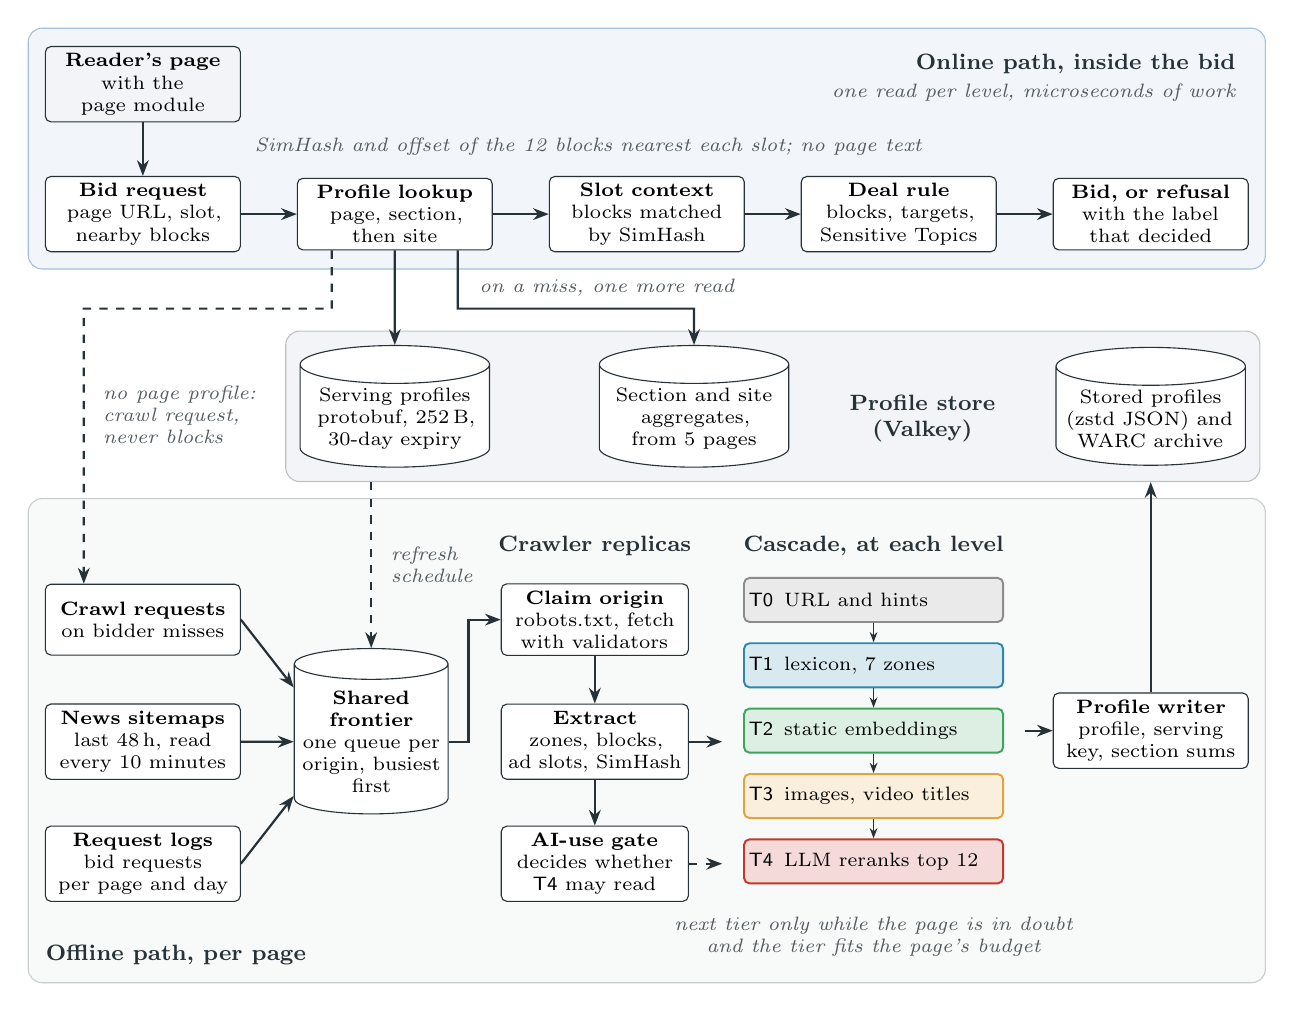
\begin{tikzpicture}[x=1cm,y=1cm,font=\scriptsize]
\tikzset{
  ovbox/.style={box,font=\scriptsize,fill=white,text width=#1,minimum height=9mm,inner sep=2.5pt},
  ovbox/.default=2.3cm,
  ovstore/.style={store,font=\scriptsize,fill=white,text width=#1,minimum height=12mm,inner sep=1.5pt},
  ovstore/.default=2.3cm,
  ovtier/.style={box,font=\scriptsize,draw=#1,fill=#1!18,line width=0.7pt,text width=3.15cm,
    minimum height=5.6mm,inner sep=2pt,align=left},
  ovlabel/.style={font=\footnotesize\bfseries,text=ink},
  ovgroup/.style={draw=ink!45,dashed,rounded corners=3pt,inner sep=4pt},
  ovstep/.style={-{Stealth[length=1.3mm]},semithick,draw=ink},
  ovnote/.style={note,font=\scriptsize\itshape},
}

% ---------------- online path ----------------
\node[ovbox] (req)  at (1.35,0)  {\textbf{Bid request}\\page URL, slot,\\nearby blocks};
\node[ovbox] (look) at (4.55,0)  {\textbf{Profile lookup}\\page, section,\\then site};
\node[ovbox] (slot) at (7.75,0)  {\textbf{Slot context}\\blocks matched\\by SimHash};
\node[ovbox] (rule) at (10.95,0) {\textbf{Deal rule}\\blocks, targets,\\Sensitive Topics};
\node[ovbox] (bid)  at (14.15,0) {\textbf{Bid, or refusal}\\with the label\\that decided};
\node[ovbox,fill=soft] (mod) at (1.35,1.65) {\textbf{Reader's page}\\with the page module};
\foreach \a/\b in {req/look,look/slot,slot/rule,rule/bid} \draw[arrow] (\a) -- (\b);
\draw[arrow] (mod) -- (req);
\node[ovnote,anchor=west] at (2.65,0.86) {SimHash and offset of the 12 blocks nearest each slot; no page text};
\node[ovlabel,anchor=north east] (onl) at (15.35,2.15) {Online path, inside the bid};
\node[ovnote,anchor=north east] at (15.35,1.78) {one read per level, microseconds of work};

% ---------------- profile store ----------------
\node[ovstore] (serv) at (4.55,-2.6)  {Serving profiles\\protobuf, 252\,B,\\30-day expiry};
\node[ovstore] (agg)  at (8.35,-2.6)  {Section and site\\aggregates,\\from 5 pages};
\node[ovlabel,align=center] (storel) at (11.25,-2.6) {Profile store\\(Valkey)};
\node[ovstore] (full) at (14.15,-2.6) {Stored profiles\\(zstd JSON) and\\WARC archive};

\draw[arrow] (look.south) -- (serv.north);
\draw[arrow] ([xshift=8mm]look.south) |- (8.35,-1.2) -- (agg.north);
\node[ovnote,anchor=south west] at (5.5,-1.17) {on a miss, one more read};

% ---------------- offline path ----------------
\node[ovbox] (d1) at (1.35,-5.15) {\textbf{Crawl requests}\\on bidder misses};
\node[ovbox] (d2) at (1.35,-6.70) {\textbf{News sitemaps}\\last 48\,h, read\\every 10 minutes};
\node[ovbox] (d3) at (1.35,-8.25) {\textbf{Request logs}\\bid requests\\per page and day};
\draw[dashedarrow] ([xshift=-8mm]look.south) |- (0.6,-1.2) -- ([xshift=-7.5mm]d1.north);
\node[ovnote,anchor=west,align=left] at (0.72,-2.55) {no page profile:\\crawl request,\\never blocks};

\node[ovstore=1.85cm,minimum height=21mm] (front) at (4.25,-6.70) {\textbf{Shared}\\\textbf{frontier}\\one queue per\\origin, busiest\\first};

\node[ovbox=2.2cm] (c1) at (7.09,-5.15) {\textbf{Claim origin}\\robots.txt, fetch\\with validators};
\node[ovbox=2.2cm] (c2) at (7.09,-6.70) {\textbf{Extract}\\zones, blocks,\\ad slots, SimHash};
\node[ovbox=2.2cm] (c3) at (7.09,-8.25) {\textbf{AI-use gate}\\decides whether\\\tier{4} may read};
\node[ovlabel] (cl) at (7.09,-4.22) {Crawler replicas};

\node[ovtier=tzero]  (t0) at (10.63,-4.90) {\tier{0}\enspace URL and hints};
\node[ovtier=tone]   (t1) at (10.63,-5.73) {\tier{1}\enspace lexicon, 7 zones};
\node[ovtier=ttwo]   (t2) at (10.63,-6.56) {\tier{2}\enspace static embeddings};
\node[ovtier=tthree] (t3) at (10.63,-7.39) {\tier{3}\enspace images, video titles};
\node[ovtier=tfour]  (t4) at (10.63,-8.22) {\tier{4}\enspace LLM reranks top 12};
\node[ovlabel] (casl) at (10.63,-4.22) {Cascade, at each level};
\foreach \a/\b in {t0/t1,t1/t2,t2/t3,t3/t4} \draw[ovstep] (\a.south) -- (\b.north);

\node[ovbox] (wr) at (14.15,-6.56) {\textbf{Profile writer}\\profile, serving\\key, section sums};

\begin{scope}[on background layer]
  \node[ovgroup,fit=(cl)(c1)(c3)] (cgrp) {};
  \node[ovgroup,fit=(casl)(t0)(t4)] (casc) {};
\end{scope}

\draw[arrow] (d1.east) -- (front.145);
\draw[arrow] (d2.east) -- (front.west);
\draw[arrow] (d3.east) -- (front.215);
\draw[arrow] (front.east) -- ++(0.25,0) |- (c1.west);
\draw[arrow] (c1) -- (c2);
\draw[arrow] (c2) -- (c3);
\draw[arrow] (c2.east) -- (c2.east -| casc.west);
\draw[dashedarrow] (c3.east) -- (c3.east -| casc.west);
\draw[arrow] (casc.east |- wr.west) -- (wr.west);
\node[ovnote,align=center,anchor=north] at (10.63,-8.80) {next tier only while the page is in doubt\\and the tier fits the page's budget};

% ---------------- lanes ----------------
\coordinate (offbot) at (0.2,-9.55);
\begin{scope}[on background layer]
  \node[draw=accent!40,fill=accent!6,rounded corners=5pt,inner sep=6pt,fit=(mod)(req)(bid)(onl)] (lon) {};
  \node[draw=ink!30,fill=soft,rounded corners=5pt,inner sep=5pt,fit=(serv)(full)] (lst) {};
  \node[draw=ink!25,fill=ink!3,rounded corners=5pt,inner sep=6pt,fit=(d1)(d3)(cgrp)(casc)(wr)(offbot)] (loff) {};
\end{scope}
\node[ovlabel,anchor=south west] at ([xshift=3pt,yshift=3pt]loff.south west) {Offline path, per page};

\draw[arrow] (wr.north) -- (wr.north |- lst.south);
\draw[dashedarrow] (front.north |- lst.south) -- (front.north);
\node[ovnote,anchor=west,align=left] at (4.38,-4.45) {refresh\\schedule};
\end{tikzpicture}
\caption{The two paths of \sys. Read the bottom lane left to right: pages enter a shared frontier from three sources, crawler replicas fetch and extract them, and the cascade labels them cheapest tier first, in the tier colours used in every figure. The writer fills the store in the middle, which the online path at the top reads with one key-value read per level. The dashed arrows close the loops: a profile miss becomes a crawl request, the refresh schedule sends pages with traffic back to the frontier, and the AI-use gate decides only whether \tier{4} may read the page.}
\label{fig:overview-arch}
\end{figure}

\subsection{Architecture}\label{sec:overview-arch}

The offline path is a set of crawler replicas that keep all their state in Valkey: the frontier, a politeness schedule per origin, the robots.txt and licence caches, and the profiles. Any replica can claim any origin, so the crawl grows by adding replicas. Pages enter the frontier from three sources, each with a count of bid requests per day that orders the queue: crawl requests the bidder publishes when it finds no profile, news sitemaps of busy publishers rescanned every 10 minutes, and daily traffic per page from the request logs. The first two make \ref{req:fresh} reachable (\cref{sec:crawl}). A replica claims an origin once its politeness delay has passed, checks robots.txt, fetches the page with its last validators, and extracts weighted zones, blocks in reading order with a main-content flag, the template's ad containers, and a 64-bit SimHash of the main text. The AI-use gate reads the publisher's aipref preferences, Content Signals and RSL licences; the most restrictive answer decides whether the LLM may see the page.

The cascade runs its tiers cheapest first. \tier{0} reads the URL and sitemap hints without a fetch, \tier{1} matches a reviewed lexicon over the zones, \tier{2} compares static embeddings with taxonomy prototypes, \tier{3} scores images that lack usable alt text with SigLIP 2 and reads video titles, and \tier{4} asks an LLM to rerank a shortlist of 12 labels, quoting the page for each. A page stops once it is settled, with some label confidently in and none in doubt, or once the next tier no longer fits its budget (\cref{sec:cascade}). Each page runs at several levels, which are presets of the same cascade. \preset{zero\_fetch} runs \tier{0} alone, at no cost. \preset{standard} runs \tier{0} to \tier{2} on the CPU within $10^{-5}$ USD. \preset{rich} spends what the page earns, between \preset{standard}'s budget and $5\times10^{-4}$ USD, which buys images and the LLM for busy pages; it is the level the bidder reads. \preset{deep} has $10^{-2}$ USD and freezes nothing, so every tier checks every label again; it serves golden sets and audits.

The writer stores the full profile and a compact serving profile under a key built from the bidder's own URL normalisation, reproduced byte for byte, and adds the page's scores to running sums for its top section and its site; from five pages on, their mean is served under a key of its own. Raw pages are archived as WARC records, so a page can be classified again without a new fetch.

The online path runs inside the bidder through a Go SDK, which reads the page's profile and, on a miss, the section's and then the site's. When a page module runs in the reader's browser, the bid request also carries the fingerprints and offsets of the 12 blocks nearest each slot, and the SDK turns them into the slot's own context (\cref{sec:boundary}). A deal's rule then checks blocks, Sensitive Topics and targets, and returns a verdict with the label that decided it. On an Apple M4 the key and the decoding take 83\,ns each, the rule 9\,ns and the slot context 1.8\,\textmu s, so the network read dominates (\cref{sec:serving}). The SDK is tested against fixtures written by the OCaml side; wiring it into a production bidder is the next step.

\subsection{The life of a page}\label{sec:overview-life}

Take a new article in the football section of a sports daily. Its first bid request finds no page profile, so the bidder backs off to the section, whose mean profile already says Soccer and, through the ancestors, Sports. A deal that targets Sports can take the request at once, and the miss sends a crawl request; if the publisher's news sitemap is watched, the page may already be queued. A replica fetches the page at the origin's next politeness slot and runs every level. As the page has bid traffic, \preset{rich} gets a budget from its request count at assumed rates for impressions and price; a page with a handful of requests a day affords an LLM call. Images are fetched only if a level is still in doubt after the text tiers and can afford one. Once the profile is written, the bidder's lookups hit the page itself.

The page then joins the refresh schedule: every 2 hours for 48 hours after publication, then after a day, with the interval doubling at each unchanged fetch up to 14 days. A 304 response, or a main text whose SimHash moved by at most 3 bits under the same pipeline version, means the page is not classified again; its keys simply live 30 more days. A page whose traffic stops is not fetched again, and its serving key expires after 30 days. Home pages, live blogs and section fronts are not chased: their page key is dropped, the bidder backs off to their section, and they are fetched once a day.

\subsection{Anatomy of a profile}\label{sec:overview-profile}

A profile has two forms (\cref{fig:overview-profile}). The stored profile is for people: the lab, audits and the golden set. It keeps all levels side by side, so a page can be compared at every depth, and every label keeps its evidence. Blocks always keep every Sensitive Topics label above 0.3, because suitability is never cut, and a slot inside an \code{<article>} takes that story as its page. The gate verdict says whether the LLM could read the page, and why. The pipeline version hashes the taxonomy, the lexicon and model files, the calibration, the thresholds, the presets, the image settings and the LLM's name; equal content under an equal version gives equal labels, so an unchanged page is never paid for twice. The serving profile is for the bid. It keeps the labels of \preset{rich} with their ancestors, so a rule on a parent node is a lookup of one identifier, and the labelled blocks without any text, in 252 bytes on average.

\begin{figure}[t]
\centering
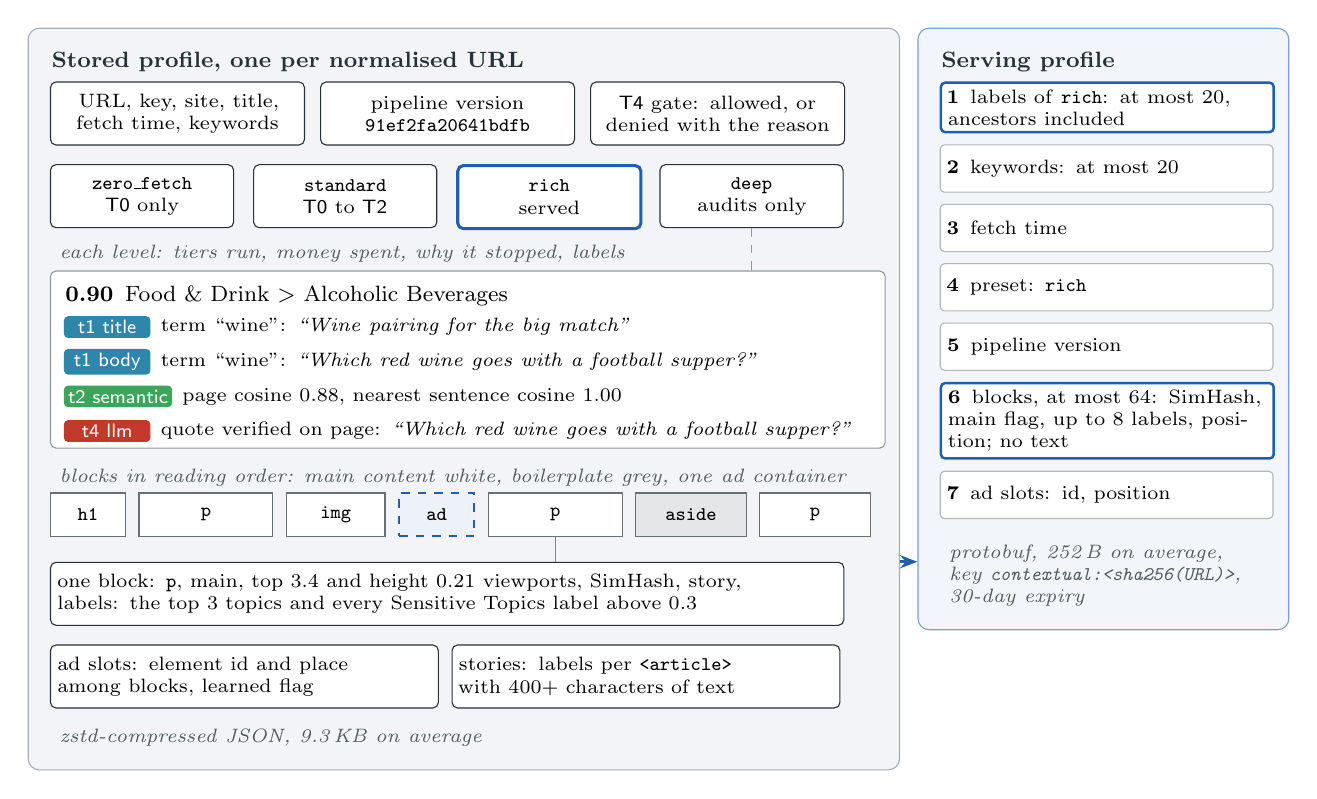
\begin{tikzpicture}[x=1cm,y=1cm,font=\scriptsize]
\tikzset{
  pfchip/.style={box,font=\scriptsize,fill=white,inner sep=2.5pt,minimum height=8mm,align=center},
  pftag/.style={font=\scriptsize\sffamily,text=white,fill=#1,rounded corners=1.5pt,inner sep=1.5pt,
    minimum width=11mm,align=center},
  pfblock/.style={draw=ink!70,fill=white,minimum height=5.5mm,inner sep=1pt,font=\scriptsize\ttfamily},
  pftitle/.style={font=\footnotesize\bfseries,text=ink,anchor=north west},
  pfnote/.style={note,font=\scriptsize\itshape},
  pffield/.style={draw=ink!35,fill=white,rounded corners=1.5pt,text width=4.05cm,inner sep=2.5pt,
    align=left,font=\scriptsize,minimum height=6mm},
}

% ---------------- stored profile ----------------
\node[pftitle] (st) at (0.15,0) {Stored profile, one per normalised URL};
\node[pfchip,text width=3.05cm,anchor=north west] (hd) at (0.25,-0.5)
  {URL, key, site, title,\\fetch time, keywords};
\node[pfchip,text width=3.05cm,anchor=north west] (ver) at (3.68,-0.5)
  {pipeline version\\\code{91ef2fa20641bdfb}};
\node[pfchip,text width=3.05cm,anchor=north west] (gate) at (7.11,-0.5)
  {\tier{4} gate: allowed, or\\denied with the reason};

\node[pfchip,text width=2.15cm,anchor=north west] (l0) at (0.25,-1.55) {\preset{zero\_fetch}\\\tier{0} only};
\node[pfchip,text width=2.15cm,anchor=north west] (l1) at (2.83,-1.55) {\preset{standard}\\\tier{0} to \tier{2}};
\node[pfchip,text width=2.15cm,anchor=north west,draw=accent,line width=1.1pt] (l2) at (5.41,-1.55) {\preset{rich}\\served};
\node[pfchip,text width=2.15cm,anchor=north west] (l3) at (7.99,-1.55) {\preset{deep}\\audits only};
\node[pfnote,anchor=north west] (ln) at (0.25,-2.45) {each level: tiers run, money spent, why it stopped, labels};

% one label with its evidence (prototype test page, deep level)
\node[draw=ink!50,fill=white,rounded corners=2pt,minimum width=10.6cm,minimum height=2.25cm,anchor=north west] (lab) at (0.25,-2.9) {};
\node[anchor=north west,font=\footnotesize] at ([xshift=2pt,yshift=-2pt]lab.north west)
  {\textbf{0.90}\enspace Food \& Drink $>$ Alcoholic Beverages};
\node[pftag=tone,anchor=west]  (e1) at (0.42,-3.62) {t1 title};
\node[anchor=west] at (e1.east) {term ``wine'': \emph{``Wine pairing for the big match''}};
\node[pftag=tone,anchor=west]  (e2) at (0.42,-4.06) {t1 body};
\node[anchor=west] at (e2.east) {term ``wine'': \emph{``Which red wine goes with a football supper?''}};
\node[pftag=ttwo,anchor=west]  (e3) at (0.42,-4.50) {t2 semantic};
\node[anchor=west] at (e3.east) {page cosine 0.88, nearest sentence cosine 1.00};
\node[pftag=tfour,anchor=west] (e4) at (0.42,-4.94) {t4 llm};
\node[anchor=west] at (e4.east) {quote verified on page: \emph{``Which red wine goes with a football supper?''}};
\draw[dashed,ink!50] (l3.south) -- (l3.south |- lab.north);

% blocks in reading order
\node[pfnote,anchor=north west] (bn) at (0.25,-5.3) {blocks in reading order: main content white, boilerplate grey, one ad container};
\node[pfblock,minimum width=0.95cm,anchor=north west] (b1) at (0.25,-5.72) {h1};
\node[pfblock,minimum width=1.7cm,anchor=west] (b2) at ([xshift=1.6mm]b1.east) {p};
\node[pfblock,minimum width=1.25cm,anchor=west] (b3) at ([xshift=1.6mm]b2.east) {img};
\node[draw=accent,dashed,thick,fill=accent!8,minimum height=5.5mm,minimum width=0.95cm,anchor=west,font=\scriptsize\ttfamily,inner sep=1pt] (ad) at ([xshift=1.6mm]b3.east) {ad};
\node[pfblock,minimum width=1.7cm,anchor=west] (b4) at ([xshift=1.6mm]ad.east) {p};
\node[pfblock,minimum width=1.4cm,anchor=west,fill=ink!12] (b5) at ([xshift=1.6mm]b4.east) {aside};
\node[pfblock,minimum width=1.4cm,anchor=west] (b6) at ([xshift=1.6mm]b5.east) {p};
\node[pfchip,text width=9.9cm,anchor=north west,align=left] (bd) at (0.25,-6.6)
  {one block: \code{p}, main, top 3.4 and height 0.21 viewports, SimHash, story,\\labels: the top 3 topics and every Sensitive Topics label above 0.3};
\draw[ink!60] (b4.south) -- (b4.south |- bd.north);

\node[pfchip,text width=4.75cm,anchor=north west,align=left] (ads) at (0.25,-7.65)
  {ad slots: element id and place\\among blocks, learned flag};
\node[pfchip,text width=4.75cm,anchor=north west,align=left] (sto) at (5.35,-7.65)
  {stories: labels per \code{<article>}\\with 400+ characters of text};
\node[pfnote,anchor=north west] (stn) at (0.25,-8.6) {zstd-compressed JSON, 9.3\,KB on average};

% ---------------- serving profile ----------------
\node[pftitle] (sv) at (11.45,0) {Serving profile};
\node[pffield,anchor=north west,draw=accent,line width=0.9pt] (f1) at (11.55,-0.5) {\textbf{1}\enspace labels of \preset{rich}: at most 20, ancestors included};
\node[pffield,anchor=north west] (f2) at ([yshift=-1.4mm]f1.south west) {\textbf{2}\enspace keywords: at most 20};
\node[pffield,anchor=north west] (f3) at ([yshift=-1.4mm]f2.south west) {\textbf{3}\enspace fetch time};
\node[pffield,anchor=north west] (f4) at ([yshift=-1.4mm]f3.south west) {\textbf{4}\enspace preset: \preset{rich}};
\node[pffield,anchor=north west] (f5) at ([yshift=-1.4mm]f4.south west) {\textbf{5}\enspace pipeline version};
\node[pffield,anchor=north west,draw=accent,line width=0.9pt] (f6) at ([yshift=-1.4mm]f5.south west) {\textbf{6}\enspace blocks, at most 64: SimHash, main flag, up to 8 labels, position; no text};
\node[pffield,anchor=north west] (f7) at ([yshift=-1.4mm]f6.south west) {\textbf{7}\enspace ad slots: id, position};
\node[pfnote,anchor=north west,align=left] (svn) at ([yshift=-2mm]f7.south west)
  {protobuf, 252\,B on average,\\key \code{contextual:<sha256(URL)>},\\30-day expiry};

\begin{scope}[on background layer]
  \node[draw=ink!40,fill=soft,rounded corners=4pt,inner sep=5pt,fit=(st)(hd)(gate)(lab)(bd)(sto)(stn)] (stbox) {};
  \node[draw=accent!60,fill=accent!6,rounded corners=4pt,inner sep=5pt,fit=(sv)(f1)(f7)(svn)] (svbox) {};
\end{scope}
\draw[-{Stealth[length=2.2mm]},line width=1.2pt,accent] (stbox.east |- bd.north) -- (svbox.west |- bd.north);
\end{tikzpicture}
\caption{What a profile holds. Left, the stored profile: all four levels side by side, one label of the \preset{deep} level opened to show its evidence records in the tier colours (a test page of the prototype), and the page's blocks with one block opened. Right, the serving profile the bidder reads, field by field. Look at the two outlined fields: only the labels of \preset{rich} and the blocks, stripped of their text, cross into the bid.}
\label{fig:overview-profile}
\end{figure}

% 04-crawl
\section{Crawling, extraction and archiving}\label{sec:crawl}

The cascade can only label pages it has read. This section is about getting them: which pages to fetch first, how a fleet of crawlers shares one queue without breaking a site's politeness, what a publisher allows us to do with its text, what we pull out of the HTML, and when a page is worth fetching again.

\subsection{Which pages, and how fast}\label{sec:crawl-which}

Pages matter in proportion to the bid requests that carry them. On real exchange traffic, millions of distinct pages carry a bid request each day once URLs are normalised as the bidder normalises them. The traffic is concentrated: a small head of busy pages carries most of the requests, and a long tail of pages is seen only a few times. It is also new. A large share of each day's requests is on pages that had no request in the previous week.

New pages are where timing matters. A page that will become busy builds its traffic over hours: little of its first two days of requests arrives in the hour of its first request, and most arrives within a day. A profile ready an hour after the first request misses almost nothing; one ready the next morning misses most of the page's life. The long tail behaves the other way. A page that will only ever get a few requests gets most of them at once. No crawl is fast enough for those, and they are worth little.

This shapes discovery. A queue filled from yesterday's logs reaches a new page after most of its traffic. Three sources feed the frontier instead, ordered by how early they see a page. First, a crawl request on every profile miss: when the bidder looks up a page and finds nothing, it publishes the URL on a message queue, at most once per page and without ever blocking the bid (\cref{sec:serving-crawl}). A busy page's first requests arrive while it is still quiet, so the crawl starts in time. Second, news sitemaps: every ten minutes the crawler reads the sitemaps of the busiest publishers and queues the pages they date in the last 48 hours, from publication dates or \code{lastmod}, publishers with the most new pages first. Third, the request logs themselves, which rank everything else by traffic. Ordinary sitemaps and same-host links fill the gaps.

\subsection{One frontier for many crawlers}\label{sec:crawl-frontier}

Any number of crawler processes share one frontier held in the key-value store. Two goals pull against each other. The busiest page should go first, and no site should see more than one request at a time from us, at most one per second or per its \code{Crawl-delay}, whichever is longer. The frontier therefore has two levels (\cref{fig:crawl-frontier}). Each origin has its own queue, a sorted set of URLs scored by minus their bid requests a day. A second sorted set holds the origins with work, scored by the earliest time each may be fetched again. A worker claims in one Lua script, which the store runs atomically. It looks at up to 64 origins that are due, takes the one whose next URL is busiest, pops that URL, pushes the origin's next allowed time forward by a lease, and records the claim with its time. After the fetch, the worker releases the origin: it becomes due again after $\max(1\,\mathrm{s}, \text{Crawl-delay})$.

\begin{figure}[t]
\centering
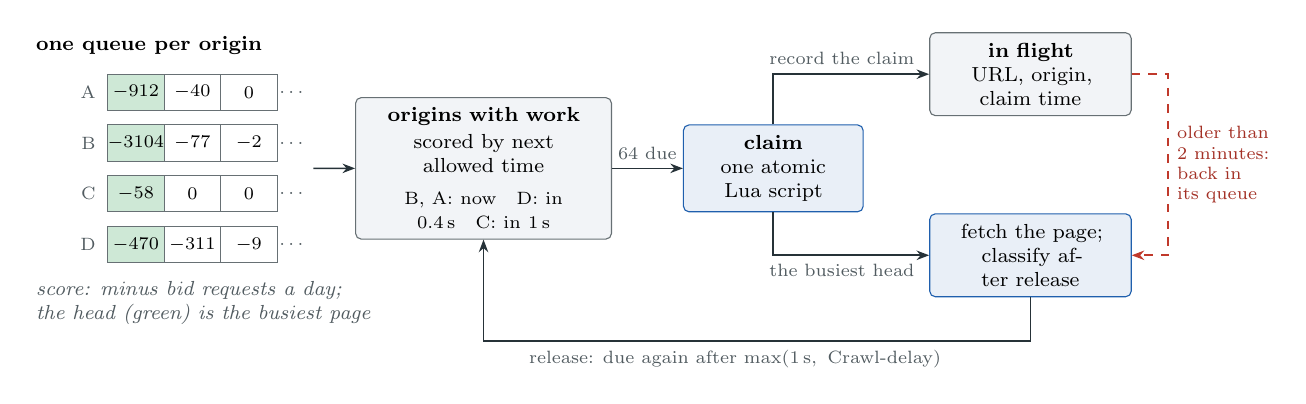
\begin{tikzpicture}[x=1cm,y=1cm,font=\footnotesize,scale=0.92,transform shape]
\tikzset{
  fq/.style={draw=ink!70, fill=white, minimum width=0.78cm, minimum height=0.5cm, inner sep=0pt, font=\scriptsize},
  fz/.style={draw=ink!70, rounded corners=2pt, fill=soft, align=center, inner sep=4pt, font=\footnotesize},
  fw/.style={draw=accent, fill=accent!10, rounded corners=2pt, align=center, inner sep=4pt, font=\footnotesize},
  fl/.style={-{Stealth[length=1.6mm]}, semithick, draw=ink},
  ft/.style={font=\scriptsize, text=ink!80},
}
\node[font=\footnotesize\bfseries, anchor=west] at (-0.95,3.75) {one queue per origin};
\foreach \o/\y/\a/\b/\c in {A/3.1/$-912$/$-40$/0, B/2.4/$-3104$/$-77$/$-2$, C/1.7/$-58$/0/0, D/1.0/$-470$/$-311$/$-9$} {
  \node[anchor=east, ft] at (0.12,\y) {\o};
  \node[fq, fill=ttwo!25] at (0.55,\y) {\a};
  \node[fq] at (1.33,\y) {\b};
  \node[fq] at (2.11,\y) {\c};
  \node[ft] at (2.72,\y) {\dots};
}
\node[note, anchor=north west, align=left] at (-0.95,0.62) {score: minus bid requests a day;\\the head (green) is the busiest page};

\node[fz, text width=3.25cm] (hosts) at (5.35,2.05) {\textbf{origins with work}\\[1pt] scored by next allowed time\\[3pt]
  {\scriptsize B, A: now\quad D: in 0.4\,s\quad C: in 1\,s}};
\node[fw, text width=2.2cm] (claim) at (9.35,2.05) {\textbf{claim}\\one atomic\\Lua script};
\node[fz, text width=2.5cm] (infl) at (12.9,3.35) {\textbf{in flight}\\URL, origin,\\claim time};
\node[fw, text width=2.5cm] (fetch) at (12.9,0.85) {fetch the page;\\classify after release};

\draw[fl] (3.0,2.05) -- (hosts.west);
\draw[fl] (hosts.east) -- node[above, ft] {64 due} (claim.west);
\draw[fl] (claim.north) |- node[pos=0.72, above, ft] {record the claim} (infl.west);
\draw[fl] (claim.south) |- node[pos=0.72, below, ft] {the busiest head} (fetch.west);
\draw[fl] (fetch.south) -- ++(0,-0.6) -| node[pos=0.27, below, ft] {release: due again after $\max(1\,\mathrm{s},\ \text{Crawl-delay})$} (hosts.south);
\draw[fl, dashed, draw=tfour] (infl.east) -- ++(0.5,0) |- node[pos=0.25, right, ft, align=left, text=tfour!85!black] {older than\\2 minutes:\\back in\\its queue} (fetch.east);
\end{tikzpicture}
\caption{The shared frontier. A claim picks, among the origins due now, the one whose next page is busiest, and takes that page in one atomic step. The origin stays leased until the fetch ends; then it is due again after the politeness delay. A claim older than two minutes belongs to a crawler that died, and any replica's housekeeping puts the page back.}
\label{fig:crawl-frontier}
\end{figure}

Because every step that touches more than one key is a single script, two replicas never fetch the same URL or the same origin at once, and the politeness interval holds across machines. On the three-board cluster of \cref{sec:impl}, three replicas crawled 15 pages from 3 sites with every page fetched once and fetches to one origin at least 1.07\,s apart. A seen-set queues each normalised URL once in the whole fleet. A page already waiting moves up when a newer count says it is busier.

\subsection{robots.txt}\label{sec:crawl-robots}

Every fetch, page, image, sitemap or licence, is checked against the site's robots.txt under RFC~9309 \citep{rfc9309}, cached for 24 hours and shared by every replica. A missing file allows everything; a server error or an unreachable host disallows everything. We match with Google's reference implementation of the standard, through our own adapter. The published OCaml binding re-parses the whole file for every URL. Our adapter parses each file once, keeps only the rules of groups that apply to our user agent, and replays them. That made a check about four times faster than the binding. Against the pure OCaml parser it replaced, parsing fell from 370 to 19\,$\mu$s on average and a check from 10.0 to 8.3\,$\mu$s. Speed was never the point: the crawler waits at least a second between requests to a host, and a 1\,$\mu$s check is a millionth of that. The point was correctness. The old parser got all 6 of the standard's edge cases we tested wrong.

\subsection{What a publisher allows}\label{sec:crawl-gate}

Fetching a page to classify it is ordinary crawling. Sending its text to a generative model is something publishers increasingly want a say in, and three signals now carry their answer (\cref{tab:crawl-gate}). The IETF's aipref vocabulary \citep{keller2026vocabulary} attaches usage preferences to paths through a \code{Content-Usage} line in robots.txt or a response header. Content Signals adds an \code{ai-input} preference in robots.txt. RSL \citep{rsl2025really} points to a machine-readable licence, from robots.txt, a \code{Link} header or a \code{<link rel="license">} element. Before \tier{4}, a gate reads all three for the page. The most restrictive answer wins, and the verdict, with its reason, is stored in the profile. A denied page never reaches the model at any level. Licences are fetched politely and cached for their stated maximum age, 30 days by default; a licence that cannot be fetched counts as missing for an hour, during which the page is treated as unlicensed.

\begin{table}[t]
\centering\small
\caption{The AI-use gate. Each source can allow, deny or say nothing about using the page as input to a generative model. A deny anywhere denies; with no stated preference and no licence, the page is allowed.}
\label{tab:crawl-gate}
\begin{tabularx}{\linewidth}{@{}l>{\raggedright\arraybackslash}X>{\raggedright\arraybackslash}X@{}}
\toprule
Signal & Where it is read & What denies \tier{4} \\
\midrule
aipref & \code{Content-Usage} in robots.txt, matched to the path like any rule; the response header of the page & a preference against AI training or use that covers this page \\
Content Signals & \code{Content-Signal} lines in robots.txt & \code{ai-input=no} \\
RSL licence & robots.txt \code{License:}, a \code{Link} header, \code{<link rel="license">} & a licence that does not permit AI use without terms we meet; a licence behind a licence server, which we cannot negotiate yet \\
\bottomrule
\end{tabularx}
\end{table}

The robots.txt lines of all three come out of the same pass through Google's parser, so the gate costs no extra parse. On the golden sample of \cref{sec:eval}, 41 of 383 stored pages are denied.

\subsection{Extraction}\label{sec:crawl-extract}

A page is fetched once and every free signal is taken from that one response. We parse HTML with lexbor, a C implementation of the HTML5 parsing algorithm, behind a small adapter that flattens the tree into a compact token stream for OCaml. On 36 real article pages it extracts 2.6 times faster than the tolerant tag scanner it replaced, about 1.4\,ms a page, and it is right where the scanner was wrong. The extractor fills the zones of \cref{eq:cascade-lexicon}, each with a weight: the URL's words and the request's hints (2), the title (3), the section from breadcrumbs or markup (2.5), keywords (2), the description (1.5), headings (1.5), the text describing media (1) and the body's sentences (1). Structured data is read wherever it is: JSON-LD and Open Graph, which almost every busy page carries, give titles, sections, keywords, publication dates and the page type (an article, a live blog).

The page is also cut into blocks in reading order: paragraphs, headings, images, embeds. Each block carries its tag, its text, whether it is main content, and an estimated position and height in viewports of a 390-pixel-wide phone, which \cref{sec:boundary} uses to place slots. Navigation, sidebars, ``most read'' lists and footers are kept but flagged as not main. They never count for relevance, and always for suitability. Each block also records the innermost \code{<article>} around it, so a page that holds several stories gives each story its own labels, and the element ids of ad containers (\code{div-gpt-ad-\dots}, \code{mpu}, \code{leaderboard}), so slot positions can be learned per template.

The crawler does not render pages. Rendering costs 10 to 50 times a plain fetch, and on the pages that matter the markup already says what the page is.

\subsection{Archiving}\label{sec:crawl-archive}

Every page the crawler classifies is kept as a WARC record: one gzip member per record, about 64\,KB a page, written by a vendored Rust library behind a C interface and indexed in the shared store. The archive serves three purposes. The lab shows the archived page, scripts off, with the extracted blocks and their scores drawn over it. Geometry measured on the archived page replaces the estimated layout. And any profile can be recomputed from the exact bytes it came from, which matters when a calibration changes.

\subsection{Refresh}\label{sec:crawl-refresh}

A page is fetched again only if it has bid traffic. The others are left alone, and their serving keys expire after 30 days. For a page worth refreshing, three questions come in order of cost.

\paragraph{Did the server say it changed?} The last \code{ETag} and \code{Last-Modified} go back as \code{If-None-Match} and \code{If-Modified-Since}. A \code{304 Not Modified} costs a round trip and no body. On the golden sample, 78 of 338 refreshed pages, 23\%, send these validators.

\paragraph{Did the text change?} A \code{200} is compared with the last fetch by a 64-bit SimHash of the main text \citep{charikar2002similarity}. Let $W$ be the page's words as the lexicon sees them, case and accents folded, and $h(w) \in \{0,1\}^{64}$ the 64-bit FNV-1a hash of word $w$. The fingerprint's $i$-th bit is a majority vote:
\begin{equation}\label{eq:crawl-simhash}
  \operatorname{sh}(W)_i = \mathbf{1}\Bigl[\sum_{w \in W} \bigl(2\,h(w)_i - 1\bigr) > 0\Bigr], \qquad i = 0, \dots, 63.
\end{equation}
A small edit flips few votes, so fingerprints of near-identical texts differ in few bits. We call a page unchanged when
\begin{equation}\label{eq:crawl-unchanged}
  \bigl\lVert \operatorname{sh}(W) \oplus \operatorname{sh}(W') \bigr\rVert_1 \le 3
  \quad\text{and}\quad
  \text{the pipeline version is the same},
\end{equation}
the threshold \citet{manku2007detecting} found right for 64-bit fingerprints at web scale. A classification is a function of the main text and the pipeline version (a hash over the taxonomy, lexicon, models and calibration, \cref{sec:impl}), so an unchanged page is not reclassified. Its serving keys, and its section's and site's, just get another 30 days.

\paragraph{When next?} The interval follows the page's age and its history (\cref{fig:crawl-schedule}). Let $a$ be the time since publication, from JSON-LD \code{datePublished} or \code{article:published\_time}, else since the first crawl, and $u$ the number of unchanged fetches in a row. For an article,
\begin{equation}\label{eq:crawl-interval}
  \Delta(a, u) =
  \begin{cases}
    2\,\mathrm{h} & a < 48\,\mathrm{h},\\
    \min\bigl(2^{u}\,\mathrm{d},\ 14\,\mathrm{d}\bigr) & \text{otherwise,}
  \end{cases}
\end{equation}
and a change resets $u$ to 0. The count runs through the first two days, so a young page that is never edited has two dozen unchanged fetches behind it at 48 hours and goes straight to the cap. Fourteen days stays under the 30-day expiry of the serving key, so a page with traffic never drops out of the store between fetches.

\begin{figure}[t]
\centering
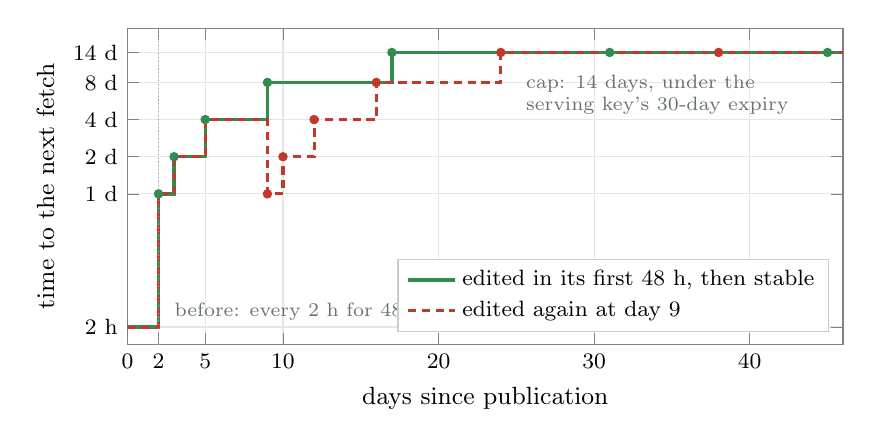
\begin{tikzpicture}
\begin{axis}[
  width=0.88\linewidth, height=5.6cm,
  xmin=0, xmax=46, ymode=log, log basis y=2, ymin=0.06, ymax=22,
  xlabel={days since publication}, ylabel={time to the next fetch},
  ytick={0.0833,1,2,4,8,14}, yticklabels={2 h,1 d,2 d,4 d,8 d,14 d},
  xtick={0,2,5,10,20,30,40},
  grid=major, grid style={ink!12}, axis line style={ink!60}, tick style={ink!60},
  ticklabel style={font=\footnotesize}, label style={font=\small},
  legend style={at={(0.98,0.04)},anchor=south east,font=\footnotesize,draw=ink!25,fill=white},
  legend cell align=left,
]
\addplot[ttwo!85!black, line width=1.2pt, const plot] coordinates {
  (0,0.0833) (2,1) (3,2) (5,4) (9,8) (17,14) (31,14) (45,14) (46,14)};
\addlegendentry{edited in its first 48 h, then stable}
\addplot[tfour, line width=1.1pt, densely dashed, const plot] coordinates {
  (0,0.0833) (2,1) (3,2) (5,4) (9,1) (10,2) (12,4) (16,8) (24,14) (38,14) (46,14)};
\addlegendentry{edited again at day 9}
\addplot[only marks, mark=*, mark size=1.5pt, ttwo!85!black, forget plot] coordinates {(2,1) (3,2) (5,4) (9,8) (17,14) (31,14) (45,14)};
\addplot[only marks, mark=*, mark size=1.5pt, tfour, forget plot] coordinates {(9,1) (10,2) (12,4) (16,8) (24,14) (38,14)};
\draw[ink!45, densely dotted] (axis cs:2,0.06) -- (axis cs:2,22);
\node[font=\scriptsize, text=ink!70, anchor=west] at (axis cs:2.4,0.11) {before: every 2 h for 48 h};
\node[font=\scriptsize, text=ink!70, anchor=north west, align=left] at (axis cs:25,11) {cap: 14 days, under the\\serving key's 30-day expiry};
\end{axis}
\end{tikzpicture}
\caption{The refresh schedule of \cref{eq:crawl-interval}, as fetch times (dots) and the interval to the next fetch (lines). A page is fetched every two hours while it is young, when it is most likely to be edited and its traffic is highest, then daily, doubling with each unchanged fetch. A change brings it back to a day.}
\label{fig:crawl-schedule}
\end{figure}

\paragraph{Hubs.} Some pages change on every fetch and are never about one thing: home pages, live blogs (\code{LiveBlogPosting} in their markup), section fronts (one-segment URLs without a publication date), and any page that moved on each of its last three fetches. We do not chase them. Their page key is dropped, so the bidder backs off to their section or site (\cref{sec:serving-backoff}), and they are fetched daily to keep counting there. A one-segment URL with a publication date stays an article: 56 of the 66 one-segment URLs of the golden sample are articles.

On the three-board cluster, with synthetic traffic on the golden sample's pages, 26 of 338 stored pages became hubs. A second wave on all 338, minutes after the first, took 45 seconds; every page came back unchanged, most of them by SimHash (88 of the last 100) and the rest by \code{304} (12), and none was reclassified. Whether a word-level SimHash moves enough on a home page over hours, rather than minutes, is still to measure. So is per-host trust in validators and \code{lastmod}, which some servers get wrong.

% 05-cascade
\section{The budgeted cascade}\label{sec:cascade}

A page profile is a set of labels from the \iab, each with a score and the evidence behind it. The labels come from five tiers. They run in order of cost, and each is paid for only while the page is still in doubt. This section gives the tiers, the rule that combines their outputs, the rule that stops the cascade, the budget that caps it, and how the scores were calibrated on the golden set of \cref{sec:eval}.

\subsection{Problem}\label{sec:cascade-problem}

Let $V$ be the 704 nodes of the taxonomy and $d$ a page. We want a set of scored labels
\begin{equation}\label{eq:cascade-profile}
  \mathcal{P}(d) = \{(v, s(v), E(v)) : v \in V,\ s(v) > \rho\},
\end{equation}
where $s(v) \in [0,1]$ should read as the probability that the page is about $v$, $\rho$ is a floor below which a label is not kept, and $E(v)$ is a list of evidence records: the tier that produced the score, the zone of the page it read, a verbatim quote and a reason. Two things make the problem harder than plain multi-label classification. Each page has a budget $B(d)$ in dollars, set by what the page is worth (\cref{sec:cascade-budget}). And the profile must be closed under ancestors, so that a page about Soccer is also about Sports: whenever $v$ is kept, every $u \in \operatorname{anc}(v)$ is kept with at least the same score.

\subsection{Five tiers}\label{sec:cascade-tiers}

\Cref{tab:cascade-tiers} lists the tiers. \tier{0} reads only what is known before any fetch: the words of the URL path and hints from sitemaps and the bid request. \tier{1} matches a lexicon of weighted terms per category against each zone of the extracted page. \tier{2} embeds the page and its first 40 text units with a static Model2Vec model \citep{tulkens2024model2vec} and compares them with one prototype per category. \tier{3} reads what text cannot: titles of embedded video, and images without usable alt text, which SigLIP~2 \citep{tschannen2025siglip} scores against every category zero-shot. \tier{4} is a small language model that reranks a shortlist.

\begin{table}[t]
\centering\small
\caption{The tiers, in the order they run. Costs are the cascade's own estimates in dollars per page, used against the budget; \tier{4}'s is the billed price of the default model. \emph{Mode} says how a tier's score meets an earlier one (\cref{eq:cascade-accumulate,eq:cascade-override}).}
\label{tab:cascade-tiers}
\begin{tabularx}{\linewidth}{@{}l>{\raggedright\arraybackslash}Xr l@{}}
\toprule
Tier & Reads & Cost & Mode \\
\midrule
\textcolor{tzero}{\textbf{\tier{0}}} URL and hints & URL path words, sitemap and request hints; no fetch & \$0 & accumulate \\
\textcolor{tone}{\textbf{\tier{1}}} lexicon & weighted terms in title, headings, body, metadata, JSON-LD & \$\num{1e-6} & accumulate \\
\textcolor{ttwo}{\textbf{\tier{2}}} dense & page and sentence embeddings against 704 prototypes & \$\num{5e-6} & override \\
\textcolor{tthree}{\textbf{\tier{3}}} media & video titles through the lexicon; up to 3 images through SigLIP~2 & \$\num{1e-4} per item & accumulate \\
\textcolor{tfour}{\textbf{\tier{4}}} LLM & a condensed page and a shortlist of 12 labels; must quote the page & \$\num{1.4e-4} per call & override \\
\bottomrule
\end{tabularx}
\end{table}

The lexicon scores a category by its accumulated term weight. If $w_z$ is the weight of zone $z$ and $w_\tau$ that of a term $\tau$ listed for $v$, the raw weight on page $d$ and the \tier{1} score are
\begin{equation}\label{eq:cascade-lexicon}
  r(v \mid d) = \sum_{z} \sum_{\tau \in z \cap \mathrm{terms}(v)} w_z\, w_\tau,
  \qquad
  s_1(v \mid d) = 1 - e^{-r(v\mid d)/k_\ell},
\end{equation}
where $k_\ell$ is a saturation that depends on the page's language $\ell$. A single mention in the body stays weak; a hit in the title and the section is already strong. Terms are gated by language: a term only fires on a page in its language, or on a page that declares none.

\tier{2} turns cosine similarity into a probability with a logistic map, Platt scaling, fitted per model and per language (\cref{sec:cascade-calibration}):
\begin{equation}\label{eq:cascade-dense}
  s_2(v \mid d) = \sigma\bigl(a_\ell\, \cos(\mathbf{e}_d, \mathbf{p}_{v,\ell}) + b_\ell\bigr),
  \qquad \sigma(x) = \frac{1}{1+e^{-x}},
\end{equation}
where $\mathbf{e}_d$ is the page embedding and $\mathbf{p}_{v,\ell}$ the prototype of $v$ in language $\ell$: the category's path plus that language's lexicon terms, embedded once. English pages use the English model; every other language uses the multilingual one, against prototypes written in that language.

\tier{4} never sees all 704 labels. Asked to pick among that many, a language model does poorly \citep{kamen2025order}. It sees the 12 labels the cheaper tiers scored highest, with their paths, and a condensed page (URL, title, description, section, keywords and the first 15 sentences), never the HTML. It must quote the page for every label it keeps. \Cref{sec:cascade-t4} gives the contract.

\subsection{How scores combine}\label{sec:cascade-combine}

The cascade keeps one running label set $L$ with scores $s(v)$. A tier returns fresh scores $f(v)$. Two modes combine them. A tier that brings independent evidence, another zone or another modality, \emph{accumulates} by noisy-OR. A tier whose model is better calibrated than what came before \emph{overrides}:
\begin{align}
  \text{accumulate:}\quad & s(v) \leftarrow 1 - \bigl(1-s(v)\bigr)\bigl(1-f(v)\bigr), \label{eq:cascade-accumulate}\\
  \text{override:}\quad & s(v) \leftarrow f(v). \label{eq:cascade-override}
\end{align}
Either way, a label already at or above the accept threshold $\alpha$ is frozen: a cheaper tier decided it, and a later one may not take it back. A label new to $L$ enters with its fresh score. Evidence lists are concatenated, so a label carries the record of every tier that touched it. When the cascade stops, labels at or below the reject threshold $\rho$ are dropped and every kept label's ancestors are added:
\begin{equation}\label{eq:cascade-finalize}
  \operatorname{final}(L) = \operatorname{cl}\bigl(\{v \in L : s(v) > \rho\}\bigr),
\end{equation}
an ancestor taking the best score among its kept descendants unless a tier scored it higher itself. \Cref{tab:cascade-toy} follows three labels through a page.

\begin{table}[t]
\centering\small
\caption{Three labels through a cascade with $\alpha = 0.8$ and $\rho = 0.3$. Soccer freezes at \tier{1} and \tier{2} cannot lower it. \tier{2} overrides Fan Conventions down, which \tier{1} had raised from a misleading phrase. Food \& Drink stays doubtful after \tier{2}, which keeps the page unsettled and pays for \tier{3}.}
\label{tab:cascade-toy}
\begin{tabular}{@{}lccccc@{}}
\toprule
Label & \tier{0} & \tier{1} (acc.) & \tier{2} (over.) & \tier{3} (acc.) & kept \\
\midrule
Sports $>$ Soccer & 0.40 & 0.40, 0.70 $\to$ \textbf{0.82} & \textbf{0.82} (frozen) & \textbf{0.82} & yes \\
Events $>$ Fan Conventions & -- & 0.35 & 0.12 & 0.12 & no \\
Food \& Drink & -- & 0.22 & 0.46 & 0.46, 0.30 $\to$ 0.62 & yes \\
\bottomrule
\end{tabular}
\end{table}

\subsection{When to stop}\label{sec:cascade-stop}

Every remaining doubt is what the next, more expensive tier is paid for. A page with no doubt left is settled.

\begin{definition}[Settled]\label{def:cascade-settled}
Under a policy $\pi = (B, \alpha, \rho)$ with $0 \le \rho < \alpha$, a label set $L$ is \emph{settled} when some label is accepted and none is doubtful:
\begin{equation}\label{eq:cascade-settled}
  \operatorname{settled}_\pi(L) \iff \bigl(\exists v \in L : s(v) \ge \alpha\bigr) \wedge \bigl(\nexists v \in L : \rho < s(v) < \alpha\bigr).
\end{equation}
\end{definition}

A settled page has at least one confident label and no label that a better tier could still move across either threshold. A page where every label sits below $\rho$ is not settled: nothing has been found, and the next tier may find something. \Cref{alg:cascade-run} is the whole loop. It is short on purpose. Before each tier it asks four questions in a fixed order, and the first that applies decides.

\begin{algorithm}[t]
\caption{The cascade for one page and one policy $\pi = (B, \alpha, \rho)$. Tiers come in cost order.}
\label{alg:cascade-run}
\begin{algorithmic}[1]
\Function{Cascade}{$d$, $\pi$, tiers $t_0, \dots, t_n$}
  \State $L \gets \emptyset$; \quad $c \gets 0$ \Comment{labels, money spent}
  \For{$i = 0, \dots, n$}
    \If{$\operatorname{settled}_\pi(L)$} \Return $(\operatorname{final}(L), c, \textsc{settled})$ \EndIf
    \If{$t_i$ does not apply to $d$} \textbf{continue} \Comment{no text units, no media: free}\EndIf
    \If{$c + \operatorname{cost}_{t_i}(d) > B$} \Return $(\operatorname{final}(L), c, \textsc{out of budget})$ \EndIf
    \State $L \gets \operatorname{update}_\alpha\bigl(L, t_i(d, L)\bigr)$ \Comment{\cref{eq:cascade-accumulate,eq:cascade-override}, frozen at $\alpha$}
    \State $c \gets c + \operatorname{cost}_{t_i}(d)$
  \EndFor
  \State \Return $(\operatorname{final}(L), c, \textsc{no more tiers})$
\EndFunction
\end{algorithmic}
\end{algorithm}

A tier receives the labels so far, $t_i(d, L)$. Only \tier{4} uses them, to build its shortlist. A tier that would exceed the budget ends the run; no later tier is tried, since later tiers cost more.

Four policies, the presets, cover the uses we have (\cref{tab:cascade-presets}). Every crawled page is run under the first three, each giving its own level of the profile, so the same page can be compared at every depth. \preset{deep} never settles, because $\alpha > 1$: every affordable tier re-checks every label. It is the audit level, and it runs only when asked.

\begin{table}[t]
\centering\small
\caption{Presets. $\alpha$ and $\rho$ are defaults; all but \preset{deep}'s are replaced per language (\cref{tab:cascade-tunings}). \preset{rich}'s budget is a ceiling: a page gets what it earns (\cref{eq:cascade-budget}).}
\label{tab:cascade-presets}
\begin{tabular}{@{}lrccl@{}}
\toprule
Preset & Budget $B$ & $\alpha$ & $\rho$ & Use \\
\midrule
\preset{zero\_fetch} & \$0 & 0.80 & 0.30 & before the page is fetched: URL and hints only \\
\preset{standard} & \$\num{1e-5} & 0.80 & 0.30 & text tiers \tier{0}--\tier{2} \\
\preset{rich} & up to \$\num{5e-4} & 0.80 & 0.30 & what the bidder reads: adds \tier{3}, and \tier{4} if earned \\
\preset{deep} & \$\num{1e-2} & 1.01 & 0.30 & audits and the golden set: nothing freezes \\
\bottomrule
\end{tabular}
\end{table}

\subsection{A budget that follows value}\label{sec:cascade-budget}

The same spend on every page wastes money on the long tail and starves the head (\ref{req:cost}). The crawler knows how many bid requests a page receives a day, $q(d)$, from the request logs and from the claim that hands it the page. With an assumed share $\eta$ of requests that become impressions and an assumed eCPM $m$ in dollars, the page earns about $\eta\, q(d)\, m / 1000$ dollars a day. The cascade may spend a fraction $\phi$ of what it earns over $D$ days, clamped between \preset{standard}'s budget and \preset{rich}'s:
\begin{equation}\label{eq:cascade-budget}
  B(d) = \min\Bigl(B_{\mathrm{rich}},\ \max\Bigl(B_{\mathrm{std}},\ \phi \, D\, \eta\, q(d)\, \frac{m}{1000}\Bigr)\Bigr).
\end{equation}
The code uses $\phi = 0.01$ and $D = 7$ days; $\eta$ and $m$ are set by the operator from its own win rate and prices. \tier{4} needs the text tiers' \num{6e-6} plus its own \num{1.4e-4}, about \num{1.5e-4}, so it becomes affordable once $\phi D \eta\, q(d)\, m/1000$ passes that, which for plausible rates means a handful of bid requests a day. A page with one or two requests a day stays at \preset{standard}'s budget and never fetches an image.

\subsection{Thresholds per language}\label{sec:cascade-tunings}

A single pair $(\alpha, \rho) = (0.8, 0.3)$ does not hold across languages. On the golden set, before \tier{4}, no Italian, French or German label reached 0.8 at \preset{deep}, so every such page would go to \tier{4}; on English pages the same cut kept 70.6\% precision. The thresholds and the \tier{1} saturation are therefore fitted per language, together, as one small constrained problem. Let $\theta_\ell = (k_\ell, \alpha_\ell, \rho_\ell)$ for each language $\ell$ with enough judged pages, and one shared $\theta$ for the rest. A page that settles at \preset{rich} serves its \tier{0}--\tier{3} labels; a page that does not is one \tier{4} sees. With $\mathcal{D}_\ell$ the judged pages in $\ell$ and $u_\theta(d) = 1$ when $d$ does not settle,
\begin{equation}\label{eq:cascade-fit}
  \max_{\{\theta_\ell\}}\ \hF\bigl(\{\theta_\ell\}\bigr)
  \quad\text{subject to}\quad
  \frac{1}{|\mathcal{D}|}\sum_\ell \sum_{d \in \mathcal{D}_\ell} u_{\theta_\ell}(d) \le 0.30,
\end{equation}
where \hF{} is the hierarchical F$_1$ of what the \preset{rich} level would serve over all judged pages, taking \tier{4}'s output from the stored \preset{deep} level for the pages it sees. The bound is the share of pages the cost model budgets for \tier{4}. Each $\theta_\ell$ ranges over a grid of 140 choices (saturation, accept, reject), and the share of \tier{4} calls is allocated across languages to the best overall \hF. \Cref{tab:cascade-tunings} gives the result.

\begin{table}[t]
\centering\small
\caption{Per-language tunings, fitted by \cref{eq:cascade-fit}. ``Others'' includes German (27 judged pages) and the rare languages. With one pair everywhere, $(4, 0.8, 0.3)$, \preset{rich} reaches \hF{} 0.544 but sends 49.1\% of pages to \tier{4}; the fit gives 0.501 at 29.8\%, cutting \tier{4}'s cost per million pages from about \$70 to \$42.}
\label{tab:cascade-tunings}
\begin{tabular}{@{}lrccccccr@{}}
\toprule
Language & Pages & $k_\ell$ & $\alpha_\ell$ & $\rho_\ell$ & \hP & \hR & \hF & \tier{4} share \\
\midrule
English & 164 & 8 & 0.5 & 0.4 & 0.545 & 0.443 & 0.489 & 22.6\% \\
Italian & 112 & 2 & 0.8 & 0.4 & 0.583 & 0.431 & 0.496 & 42.0\% \\
French & 76 & 12 & 0.5 & 0.4 & 0.690 & 0.417 & 0.520 & 26.3\% \\
Others & 31 & 12 & 0.7 & 0.4 & 0.607 & 0.546 & 0.575 & 32.3\% \\
\midrule
All & 383 & & & & 0.577 & 0.442 & 0.501 & 29.8\% \\
\bottomrule
\end{tabular}
\end{table}

Italian keeps the highest accept and still sends 42\% of its pages to \tier{4}: its \tier{0}--\tier{3} labels gain least from wider thresholds, so the allocation spends \tier{4} there. Two caveats hold for every number in this table. The fit has 140 choices per language for 31 to 164 pages, so it can overfit. And \tier{4}'s outcome comes from an older crawl, on older shortlists. We refit both when the golden set is recrawled in audit mode.

\subsection{Calibration}\label{sec:cascade-calibration}

Thresholds only mean something if scores are calibrated. A score of 0.7 should be right about 70\% of the time. We measure this with the expected calibration error over $M = 10$ equal bins \citep{guo2017calibration},
\begin{equation}\label{eq:cascade-ece}
  \mathrm{ECE} = \sum_{m=1}^{M} \frac{|B_m|}{n}\, \bigl|\operatorname{acc}(B_m) - \operatorname{conf}(B_m)\bigr|,
\end{equation}
over the $n$ labels a tier hands the cascade (score $\ge 0.3$), where $\operatorname{acc}$ is the share of labels in bin $B_m$ that are right, ancestors included, and $\operatorname{conf}$ their mean score.

\paragraph{Platt scaling.} For a raw signal $x$ (a cosine, a logit) and a label $y \in \{0,1\}$, Platt's method fits $p(y = 1 \mid x) = \sigma(ax+b)$ by maximum likelihood \citep{platt1999probabilistic}. On $n_+$ positives and $n_-$ negatives we use Platt's smoothed targets, $t_+ = (n_+ + 1)/(n_+ + 2)$ and $t_- = 1/(n_- + 2)$, so separable data keeps a finite slope, and minimise the cross-entropy
\begin{equation}\label{eq:cascade-platt}
  \ell(a, b) = -\sum_{i} \Bigl[t_i \log \sigma(a x_i + b) + (1 - t_i)\log\bigl(1 - \sigma(a x_i + b)\bigr)\Bigr]
\end{equation}
by Newton's method with step halving, as \citet{lin2007note} recommend for numerical safety. Every (page, category) pair of the golden set is one example: 704 per page, most of them negative.

\paragraph{\tier{2}.} The hand-set map before the golden set was $\sigma(25x - 6)$ for every model. It was far too steep. On an Italian football page, page cosines from 0.43 to 0.68 for a dozen Sports children all mapped to 0.999, and the cascade handed on 46 labels at 0.3 or more per page. \Cref{fig:cascade-platt} shows the fitted curves. The English model keeps a steep slope; the multilingual model, whose cosines run lower and closer together, gets a gentler one for each language. With the old map, \preset{standard} served labels at precision 0.10; with the fitted ones, at 0.45.

\begin{figure}[t]
\centering
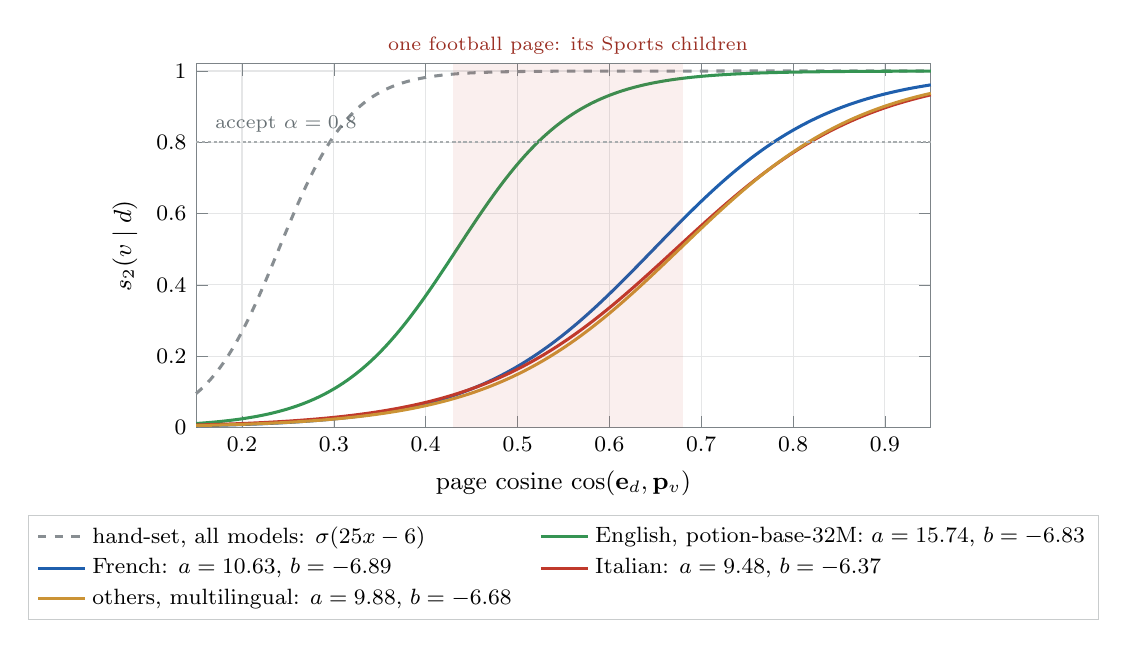
\begin{tikzpicture}
\begin{axis}[
  width=0.9\linewidth, height=6.2cm,
  xmin=0.15, xmax=0.95, ymin=0, ymax=1.02,
  xlabel={page cosine $\cos(\mathbf{e}_d, \mathbf{p}_v)$}, ylabel={$s_2(v \mid d)$},
  grid=major, grid style={ink!12},
  axis line style={ink!60}, tick style={ink!60},
  legend style={at={(0.5,-0.24)},anchor=north,font=\footnotesize,draw=ink!25,fill=white,legend columns=2,
    /tikz/every even column/.append style={column sep=8pt}},
  legend cell align=left, clip=false,
  every axis plot/.append style={line width=1.1pt, samples=200, domain=0.15:0.95},
  ticklabel style={font=\footnotesize}, label style={font=\small},
]
\addplot[ink!55, dashed] {1/(1+exp(-(25*x-6)))};
\addlegendentry{hand-set, all models: $\sigma(25x-6)$}
\addplot[ttwo!90!black] {1/(1+exp(-(15.74*x-6.83)))};
\addlegendentry{English, potion-base-32M: $a=15.74$, $b=-6.83$}
\addplot[accent] {1/(1+exp(-(10.63*x-6.89)))};
\addlegendentry{French: $a=10.63$, $b=-6.89$}
\addplot[tfour] {1/(1+exp(-(9.48*x-6.37)))};
\addlegendentry{Italian: $a=9.48$, $b=-6.37$}
\addplot[tthree!90!black] {1/(1+exp(-(9.88*x-6.68)))};
\addlegendentry{others, multilingual: $a=9.88$, $b=-6.68$}
\addplot[draw=none, fill=tfour, fill opacity=0.08, domain=0.43:0.68] {1.02} \closedcycle;
\node[font=\scriptsize, text=tfour!80!black, anchor=south] at (axis cs:0.555,1.02) {one football page: its Sports children};
\addplot[ink!40, densely dotted, line width=0.8pt, domain=0.15:0.95] {0.8};
\node[font=\scriptsize, text=ink!70, anchor=south west] at (axis cs:0.16,0.8) {accept $\alpha = 0.8$};
\end{axis}
\end{tikzpicture}
\caption{\tier{2}'s map from cosine to probability, before and after the golden set. The shaded band is where a dozen Sports children of one Italian football page fell: the hand-set map put all of them near 1, the fitted Italian map spreads them between about 0.1 and 0.5, so they stay doubtful and pay for a better tier.}
\label{fig:cascade-platt}
\end{figure}

\paragraph{\tier{3}.} SigLIP~2's probabilities for a category are tiny, because it spreads mass over 704 captions. The hand-set map was $\sigma(1.74\,x + 5.21)$ on its logit $x$, which put 0.8 at a raw probability of 0.1. The fit is much flatter, $\sigma(0.41\,x - 0.30)$, and lowers the image tier's ECE from 0.401 to 0.080. A flat map moves the operating point, so the cut for keeping an image label had to move too. At the old cut of 0.3, the fitted map dropped a clear hit in our tests, an electric car at a charging point, at 0.248. At 0.15, the new cut, the same raw probability passes as before (about 0.03), and a beach football photo at 0.10 stays out.

\paragraph{\tier{1}.} The lexicon is the worst-calibrated tier: ECE 0.414 with $k = 4$ everywhere. A single saturation fitted alone, $k = 23.4$, brings it to 0.085, but then no lexicon label ever reaches accept, \preset{rich} falls to \hF{} 0.209 and sends 89\% of pages to \tier{4}. Saturation moves with the thresholds, so it is fitted with them (\cref{eq:cascade-fit}), not alone.

\paragraph{\tier{4}.} Temperature scaling, $s \mapsto \sigma(\operatorname{logit}(s)/T)$, fits $T = 1.73$ on the shortlist, but it does not lower ECE (0.081 at $T=1$, 0.101 after). We leave $T = 1$.

\subsection{The language model as a checked reranker}\label{sec:cascade-t4}

\tier{4} is the only tier whose reasons could be invented. A language model's stated rationale need not be why it answered \citep{turpin2023language}, so we do not keep rationales. We keep quotes, because a quote can be checked. \Cref{alg:cascade-t4} gives the contract. The shortlist is the 12 best labels so far. The model answers in JSON with, for each label it keeps, a confidence and a sentence copied from the page. A label whose quote is not found in the page's normalised text keeps half its confidence. An id outside the shortlist is ignored. A shortlisted label the model leaves out scores 0, and so does a label of $L$ that did not make the shortlist: \tier{4} overrides, so it is the final word on every label not already frozen.

\begin{algorithm}[t]
\caption{\tier{4}: rerank a shortlist and check every quote. $N(\cdot)$ is the text normaliser the lexicon uses.}
\label{alg:cascade-t4}
\begin{algorithmic}[1]
\Function{Rerank}{$d$, $L$}
  \State $C \gets$ the 12 labels of $L$ with the highest scores (the taxonomy's roots if $L = \emptyset$)
  \State $A \gets \textsc{Model}(\text{instructions}, \{(v, \operatorname{path}(v)) : v \in C\}, \operatorname{condensed}(d))$ \Comment{JSON: id, confidence, quote}
  \For{$v \in C$}
    \If{$(v, \gamma, \kappa) \in A$}
      \State $f(v) \gets \operatorname{clip}_{[0,1]}(\gamma)$ \textbf{if} $N(\kappa) \subseteq N(d)$ \textbf{else} $\operatorname{clip}_{[0,1]}(\gamma)/2$
    \Else\ $f(v) \gets 0$ \Comment{not selected}
    \EndIf
  \EndFor
  \For{$v \in L \setminus C$} $f(v) \gets 0$ \Comment{not in the shortlist} \EndFor
  \State \Return $f$ \Comment{overrides; frozen labels keep their score}
\EndFunction
\end{algorithmic}
\end{algorithm}

Quote checking is cheap and catches the failure that matters. On the golden set the default model's quotes were found verbatim 94\% of the time (\cref{sec:eval-t4}). Publishers can refuse all of this. Page text goes to \tier{4} only when the page's AI-use preferences allow it (\cref{sec:crawl}); a refused page skips \tier{4} at every level.

The shortlist caps what \tier{4} can recover: a gold label outside the 12 cannot come back. On the golden set the 12 best labels before \tier{4} hold 62.7\% of the gold labels. \Cref{fig:cascade-recall} shows what longer lists would hold. Even 96 labels hold 93.1\%, so the length is not the main problem. The cheaper tiers' ranking is.

\begin{figure}[t]
\centering
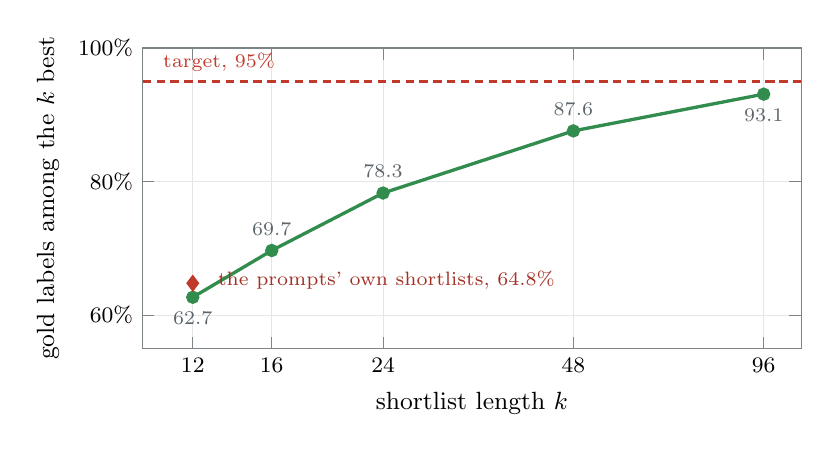
\begin{tikzpicture}
\begin{axis}[
  width=0.82\linewidth, height=5.4cm,
  xmode=log, log basis x=2,
  xmin=10, xmax=110, ymin=0.55, ymax=1.0,
  xtick={12,16,24,48,96}, xticklabels={12,16,24,48,96},
  xlabel={shortlist length $k$}, ylabel={gold labels among the $k$ best},
  grid=major, grid style={ink!12}, axis line style={ink!60}, tick style={ink!60},
  ticklabel style={font=\footnotesize}, label style={font=\small},
  yticklabel={\pgfmathparse{\tick*100}\pgfmathprintnumber[fixed,precision=0]{\pgfmathresult}\%},
]
\addplot[ttwo!85!black, line width=1.2pt, mark=*, mark size=1.8pt] coordinates {
  (12,0.627) (16,0.697) (24,0.783) (48,0.876) (96,0.931)};
\addplot[tfour, densely dashed, line width=0.9pt, domain=10:110] {0.95};
\node[font=\scriptsize, text=tfour, anchor=south west] at (axis cs:10.4,0.95) {target, 95\%};
\addplot[only marks, mark=diamond*, mark size=2.8pt, tfour] coordinates {(12,0.648)};
\node[font=\scriptsize, text=tfour!85!black, anchor=west, align=left] at (axis cs:12.7,0.652) {the prompts' own shortlists, 64.8\%};
\node[font=\scriptsize, text=ink!75, anchor=north] at (axis cs:12,0.619) {62.7};
\node[font=\scriptsize, text=ink!75, anchor=south] at (axis cs:16,0.705) {69.7};
\node[font=\scriptsize, text=ink!75, anchor=south] at (axis cs:24,0.791) {78.3};
\node[font=\scriptsize, text=ink!75, anchor=south] at (axis cs:48,0.884) {87.6};
\node[font=\scriptsize, text=ink!75, anchor=north] at (axis cs:96,0.923) {93.1};
\end{axis}
\end{tikzpicture}
\caption{Recall of the shortlist: the share of the 1,173 gold labels among the $k$ labels \tier{0}--\tier{3} score highest, before \tier{4}, at \preset{deep}. The diamond is measured on the shortlists actually sent to the model. Recall grows slowly with $k$: the ranking, not the length, keeps \tier{4} from the 95\% target.}
\label{fig:cascade-recall}
\end{figure}

\subsection{Phases, so the network never blocks a worker}\label{sec:cascade-phases}

The cascade is a pure function of the page and the tiers. It runs on a pool of CPU workers, while sockets and timers live on a single event loop (\cref{sec:impl}). \tier{4} and the image tier need the network in the middle of that function. Rather than block a worker on a remote call, the crawler splits each page into phases (\cref{alg:cascade-phases}).

\begin{algorithm}[t]
\caption{One page's levels, with network work kept out of the CPU pool.}
\label{alg:cascade-phases}
\begin{algorithmic}[1]
\State \textbf{pool:} run every level without images; note the levels still in doubt that could afford an image
\If{some such level exists and the page has images without usable alt text}
  \State \textbf{loop:} fetch up to 3 images politely; look each up in the embedding cache
  \State \textbf{pool:} embed the ones not cached, store them in the cache
\EndIf
\State \textbf{pool:} dry run of every level with a \tier{4} that records its prompt and answers nothing
\If{the page's AI-use gate allows it and some prompt was recorded}
  \State \textbf{loop:} send the prompts, collect the answers and their billed cost
\EndIf
\State \textbf{pool:} run every level for real, with the images and the answers
\end{algorithmic}
\end{algorithm}

The dry run sees exactly what the real run will send, because \tier{4} is the last tier: its prompt depends only on the tiers before it. If any call fails, \tier{4} is dropped for that page; an empty answer never zeroes the labels. Image embeddings are cached in the shared store by image URL and patch budget, 3.7\,KB each with overhead, kept 30 days, so an image that appears on many pages of a site is embedded once. On the three-board cluster of \cref{sec:impl}, with these phases and the value budget, 20\% of new pages fetched images, against every page before.

\subsection{What a page costs}\label{sec:cascade-cost}

Let $\pi_t$ be the share of pages that reach tier $t$ at \preset{rich} and $c_t$ its cost. The expected cost of a page is
\begin{equation}\label{eq:cascade-cost}
  \mathbb{E}[c] = \sum_{t=0}^{4} \pi_t\, c_t \approx \pi_4\, p_{\mathrm{call}} + \pi_3\, \bar{n}_{\mathrm{img}}\, c_{\mathrm{img}} + c_1 + c_2,
\end{equation}
where $p_{\mathrm{call}}$ is the price of one \tier{4} call and $\bar{n}_{\mathrm{img}}$ the mean number of images a page that reaches \tier{3} embeds. In money, \tier{4} dominates: with the default model billed at \$0.142 per 1,000 calls and $\pi_4 = 0.298$, it costs about \$42 per million pages. The text tiers cost \$6 per million pages in the cascade's own accounting, and images cost CPU rather than money. Billing runs about 2.7 times the catalogue price of the tokens sent, because only providers that keep no prompts are used, so the crawler's estimate of a call carries that factor.

The thresholds set $\pi_4$. \Cref{fig:cascade-grid} shows the trade-off at \preset{rich} on the golden set without \tier{4} in the loop: raising accept or reject keeps more pages unsettled, so more go to \tier{4}, while the pages that do settle serve better labels.

\begin{figure}[t]
\centering
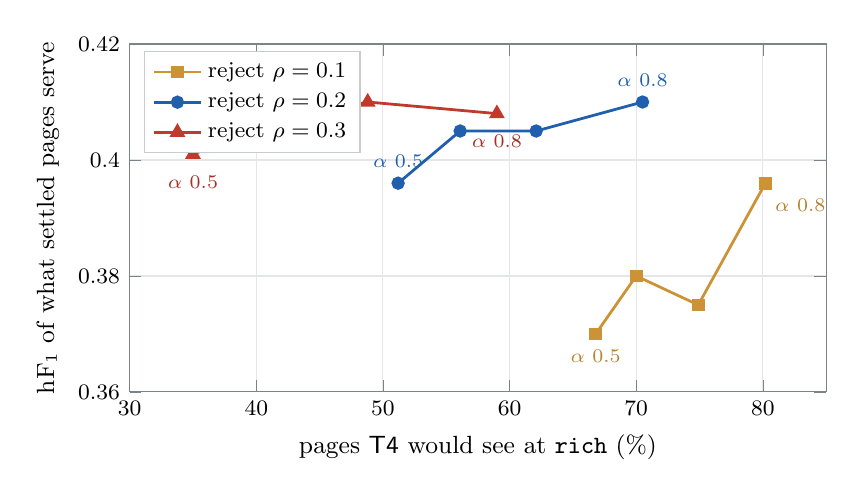
\begin{tikzpicture}
\begin{axis}[
  width=0.86\linewidth, height=6cm,
  xmin=30, xmax=85, ymin=0.36, ymax=0.42,
  xlabel={pages \tier{4} would see at \preset{rich} (\%)},
  ylabel={\hF{} of what settled pages serve},
  grid=major, grid style={ink!12}, axis line style={ink!60}, tick style={ink!60},
  ticklabel style={font=\footnotesize}, label style={font=\small},
  yticklabel style={/pgf/number format/fixed,/pgf/number format/precision=2},
  legend style={at={(0.02,0.98)},anchor=north west,font=\footnotesize,draw=ink!25,fill=white},
  legend cell align=left,
]
\addplot[tthree!90!black, line width=1pt, mark=square*, mark size=1.8pt] coordinates {(66.8,0.370) (70.0,0.380) (74.9,0.375) (80.2,0.396)};
\addlegendentry{reject $\rho = 0.1$}
\addplot[accent, line width=1pt, mark=*, mark size=1.9pt] coordinates {(51.2,0.396) (56.1,0.405) (62.1,0.405) (70.5,0.410)};
\addlegendentry{reject $\rho = 0.2$}
\addplot[tfour, line width=1pt, mark=triangle*, mark size=2.3pt] coordinates {(35.0,0.401) (41.0,0.406) (48.8,0.410) (59.0,0.408)};
\addlegendentry{reject $\rho = 0.3$}
\node[font=\scriptsize, text=tfour!85!black, anchor=north] at (axis cs:35.0,0.399) {$\alpha$ 0.5};
\node[font=\scriptsize, text=tfour!85!black, anchor=north] at (axis cs:59.0,0.406) {$\alpha$ 0.8};
\node[font=\scriptsize, text=accent, anchor=south] at (axis cs:51.2,0.397) {$\alpha$ 0.5};
\node[font=\scriptsize, text=accent, anchor=south] at (axis cs:70.5,0.411) {$\alpha$ 0.8};
\node[font=\scriptsize, text=tthree!80!black, anchor=north] at (axis cs:66.8,0.369) {$\alpha$ 0.5};
\node[font=\scriptsize, text=tthree!80!black, anchor=north west] at (axis cs:80.2,0.395) {$\alpha$ 0.8};
\end{axis}
\end{tikzpicture}
\caption{Thresholds trade \tier{4} calls for the quality of what the cheap tiers decide alone. Each point is one $(\alpha, \rho)$ at \preset{rich}, accept rising from 0.5 to 0.8 along each line, with today's calibration and no \tier{4}. A higher reject sends fewer pages to \tier{4} at almost the same quality: at $\rho = 0.3$, 35\% of pages for \hF{} 0.401, against 51\% at $\rho = 0.2$. The per-language fit of \cref{tab:cascade-tunings} uses $\rho = 0.4$.}
\label{fig:cascade-grid}
\end{figure}

\subsection{The flow, end to end}\label{sec:cascade-flow}

\Cref{fig:cascade-flow} puts the pieces together for one page at \preset{rich}.

\begin{figure}[t]
\centering
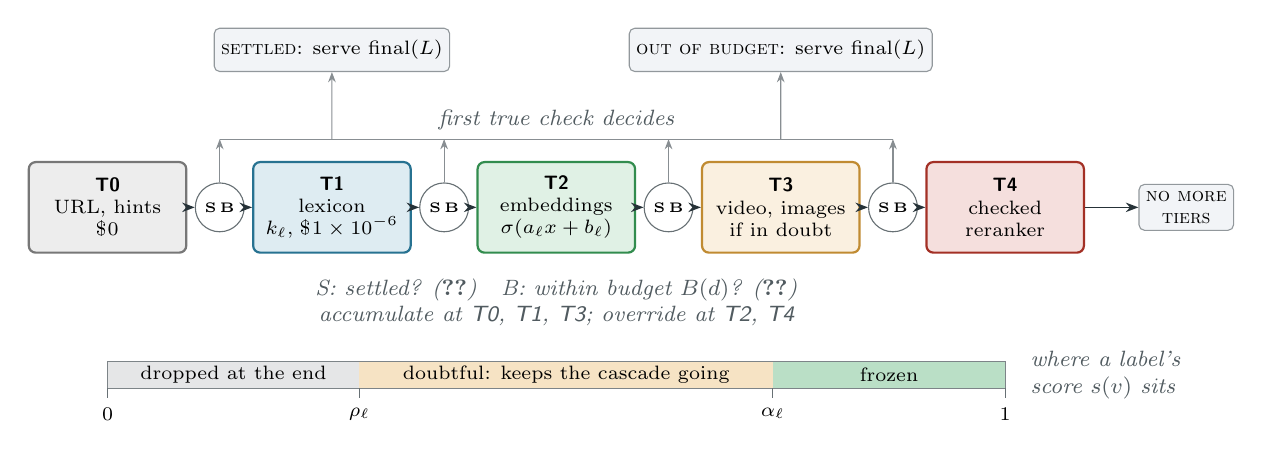
\begin{tikzpicture}[x=1cm,y=1cm,font=\scriptsize]
\tikzset{
  cTier/.style={draw=#1!85!black, fill=#1!16, line width=0.8pt, rounded corners=2.5pt,
    minimum width=2.0cm, minimum height=1.15cm, align=center, inner sep=2pt},
  cGate/.style={draw=ink!70, fill=white, circle, minimum size=6.2mm, inner sep=0pt, font=\tiny\bfseries},
  cStop/.style={draw=ink!50, fill=soft, rounded corners=2pt, minimum height=5.5mm, inner sep=2.5pt, font=\scriptsize, align=center},
  cLine/.style={-{Stealth[length=1.6mm]}, semithick, draw=ink},
  cThin/.style={-{Stealth[length=1.3mm]}, thin, draw=ink!55},
}
\node[cTier=tzero] (t0) at (0,0)    {\textbf{\tier{0}}\\URL, hints\\\$0};
\node[cTier=tone]  (t1) at (2.85,0) {\textbf{\tier{1}}\\lexicon\\$k_\ell$, \$\num{1e-6}};
\node[cTier=ttwo]  (t2) at (5.7,0) {\textbf{\tier{2}}\\embeddings\\$\sigma(a_\ell x + b_\ell)$};
\node[cTier=tthree](t3) at (8.55,0) {\textbf{\tier{3}}\\video, images\\if in doubt};
\node[cTier=tfour] (t4) at (11.4,0) {\textbf{\tier{4}}\\checked\\reranker};
\foreach \a/\b/\g in {t0/t1/g1,t1/t2/g2,t2/t3/g3,t3/t4/g4} {
  \node[cGate] (\g) at ($(\a.east)!0.5!(\b.west)$) {S\,B};
  \draw[cLine] (\a.east) -- (\g.west);
  \draw[cLine] (\g.east) -- (\b.west);
}
\node[cStop] (settled) at (2.85,2.0) {\textsc{settled}: serve $\operatorname{final}(L)$};
\node[cStop] (budget)  at (8.55,2.0) {\textsc{out of budget}: serve $\operatorname{final}(L)$};
\foreach \g in {g1,g2,g3,g4} {
  \draw[cThin] (\g.north) -- ++(0,0.55) coordinate (\g top);
}
\draw[ink!55, thin] (g1top) -- (g4top);
\draw[cThin] ($(g1top)!0.5!(g2top)$) -- (settled.south);
\draw[cThin] ($(g3top)!0.5!(g4top)$) -- (budget.south);
\node[note, anchor=south] at ($(g2top)!0.5!(g3top)$) {first true check decides};
\node[cStop] (done) at (13.7,0) {\textsc{no more}\\\textsc{tiers}};
\draw[cLine] (t4.east) -- (done.west);

% score axis
\begin{scope}[yshift=-2.3cm]
\fill[ink!12] (0,0) rectangle (3.2,0.34);
\fill[tthree!30] (3.2,0) rectangle (8.45,0.34);
\fill[ttwo!35] (8.45,0) rectangle (11.4,0.34);
\draw[ink!60] (0,0) rectangle (11.4,0.34);
\foreach \x/\l in {0/0, 3.2/$\rho_\ell$, 8.45/$\alpha_\ell$, 11.4/1} {
  \draw[ink!70] (\x,0) -- (\x,-0.12);
  \node[anchor=north, font=\scriptsize] at (\x,-0.12) {\l};
}
\node[font=\scriptsize, align=center] at (1.6,0.17) {dropped at the end};
\node[font=\scriptsize, align=center] at (5.825,0.17) {doubtful: keeps the cascade going};
\node[font=\scriptsize, align=center] at (9.925,0.17) {frozen};
\node[note, anchor=west, align=left] at (11.6,0.17) {where a label's\\score $s(v)$ sits};
\end{scope}
\node[note, anchor=north] at (5.7,-0.78) {S: settled? (\cref{eq:cascade-settled})\quad B: within budget $B(d)$? (\cref{eq:cascade-budget})\\accumulate at \tier{0}, \tier{1}, \tier{3}; override at \tier{2}, \tier{4}};
\end{tikzpicture}
\caption{The cascade for one page. Between tiers, two checks run in order: if the page is settled it stops and serves its labels; if the next tier would exceed the page's budget it stops too. \tier{3} runs only on a level still in doubt that can afford an image, and \tier{4} only when the publisher allows it. The bar below gives the meaning of a score against the language's thresholds.}
\label{fig:cascade-flow}
\end{figure}

The design leaves out two things on purpose. There is no learned combiner: the accumulate, override and freeze rules are written by hand, and the evidence they keep is what a learned stacker would need later. And the thresholds carry no statistical guarantee. Conformal methods could bound the share of wrong labels a threshold lets through \citep{angelopoulos2024conformal,angelopoulos2021learn}; they need a golden set judged by people, which is the next step of \cref{sec:eval}.

% 06-boundary
\section{Context boundaries: from the page to the slot}\label{sec:boundary}

The profile of \cref{sec:cascade} describes a URL. An ad does not see a URL.
It sits at one spot on a page, and the reader sees it together with whatever
is on screen at that moment. An interscroller opens in the middle of an
article, right after the paragraphs the reader has just read. A sidebar banner
sits next to a ``most read'' list that may have nothing to do with the
article. A full-screen interstitial covers the page and has no position in it
at all. So we ask where the context of an ad stops. Our answer is that it
stops in three places, each with its own job, and that the ad format decides
how much each one counts (\cref{fig:boundary-phone}).

\begin{figure}[t]
\centering
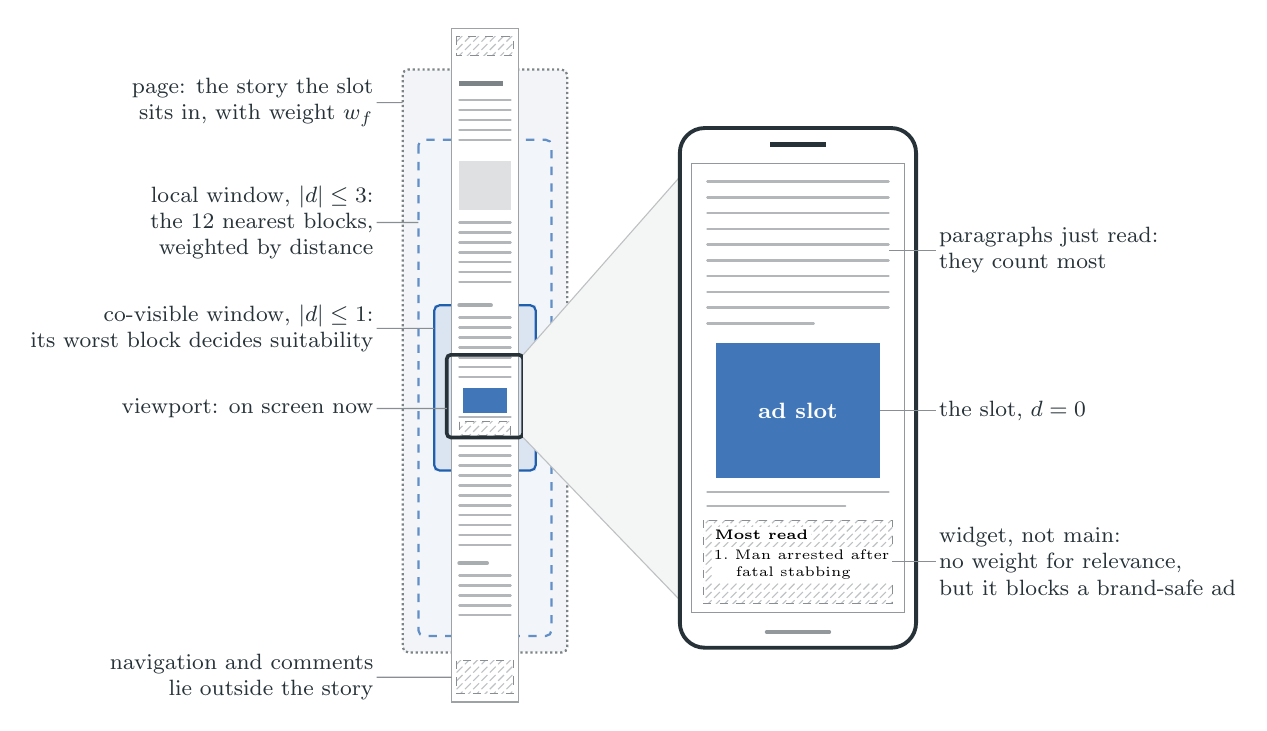
\begin{tikzpicture}[
  ln/.style={line width=0.9pt,draw=ink!35,line cap=round},
  big/.style={line width=1.5pt,draw=ink!40,line cap=round},
  hatch/.style={draw=ink!55,dashed,pattern=north east lines,pattern color=ink!30},
  lab/.style={font=\footnotesize,text=ink,align=right,anchor=east,inner sep=1pt},
  rlab/.style={font=\footnotesize,text=ink,align=left,anchor=west,inner sep=1pt},
  lead/.style={draw=ink!55,thin}]
  % Left: the whole page, to scale vertically (1 viewport = 1.05 cm).
  \begin{scope}[yscale=-1.05]
    \fill[soft] (-0.62,-3.85) rectangle (1.47,3.2);
    \draw[ink!60,densely dotted,thick,rounded corners=2pt] (-0.62,-3.85) rectangle (1.47,3.2);
    \fill[accent!6] (-0.42,-3) rectangle (1.27,3);
    \draw[accent!70,dashed,thick,rounded corners=2pt] (-0.42,-3) rectangle (1.27,3);
    \fill[accent!16] (-0.22,-1) rectangle (1.07,1);
    \draw[accent,thick,rounded corners=2pt] (-0.22,-1) rectangle (1.07,1);
    \fill[white] (0,-4.35) rectangle (0.85,3.8);
    \draw[ink!45] (0,-4.35) rectangle (0.85,3.8);
    \fill[hatch] (0.06,-4.25) rectangle (0.79,-4.02);
    \draw[ink!60,line width=2pt] (0.1,-3.68) -- (0.65,-3.68);
    \foreach \y in {-3.48,-3.36,...,-2.9} \draw[ln] (0.1,\y) -- (0.75,\y);
    \fill[ink!15] (0.1,-2.75) rectangle (0.75,-2.15);
    \foreach \y in {-2.0,-1.88,...,-1.2} \draw[ln] (0.1,\y) -- (0.75,\y);
    \draw[big] (0.1,-1.0) -- (0.5,-1.0);
    \foreach \y in {-0.85,-0.73,...,-0.1} \draw[ln] (0.1,\y) -- (0.75,\y);
    \fill[accent!85] (0.14,0) rectangle (0.71,0.30);
    \draw[ln] (0.1,0.35) -- (0.75,0.35);
    \fill[hatch] (0.1,0.41) rectangle (0.75,0.58);
    \foreach \y in {0.70,0.82,...,1.95} \draw[ln] (0.1,\y) -- (0.75,\y);
    \draw[big] (0.1,2.12) -- (0.45,2.12);
    \foreach \y in {2.27,2.39,...,2.8} \draw[ln] (0.1,\y) -- (0.75,\y);
    \fill[hatch] (0.06,3.3) rectangle (0.79,3.7);
    % The viewport.
    \draw[ink,line width=1.3pt,rounded corners=1.5pt] (-0.06,-0.40) rectangle (0.91,0.60);
    \coordinate (vt) at (0.91,-0.40);
    \coordinate (vb) at (0.91,0.60);
    % Labels.
    \node[lab] (a) at (-0.95,-3.45) {page: the story the slot\\sits in, with weight $w_f$};
    \draw[lead] (a.east) -- (-0.62,-3.45);
    \node[lab] (b) at (-0.95,-2.0) {local window, $|d|\le 3$:\\the 12 nearest blocks,\\weighted by distance};
    \draw[lead] (b.east) -- (-0.42,-2.0);
    \node[lab] (c) at (-0.95,-0.72) {co-visible window, $|d|\le 1$:\\its worst block decides suitability};
    \draw[lead] (c.east) -- (-0.22,-0.72);
    \node[lab] (e) at (-0.95,0.25) {viewport: on screen now};
    \draw[lead] (e.east) -- (-0.06,0.25);
    \node[lab] (f) at (-0.95,3.5) {navigation and comments\\lie outside the story};
    \draw[lead] (f.east) -- (0,3.5);
  \end{scope}
  % Right: the viewport, enlarged, as the reader's phone shows it.
  \fill[ink!5] (vt) -- (3.05,2.85) -- (3.05,-2.85) -- (vb) -- cycle;
  \draw[ink!30] (vt) -- (3.05,2.85) (vb) -- (3.05,-2.85);
  \draw[ink,line width=1.4pt,fill=white,rounded corners=9pt] (2.9,-3.3) rectangle (5.9,3.3);
  \fill[ink] (4.05,3.06) rectangle (4.75,3.12);
  \draw[ink!50,line width=1.2pt,line cap=round] (4.0,-3.1) -- (4.8,-3.1);
  \draw[ink!50] (3.05,-2.85) rectangle (5.75,2.85);
  \foreach \y in {2.62,2.42,...,1.0} \draw[ln] (3.25,\y) -- (5.55,\y);
  \draw[ln] (3.25,0.82) -- (4.6,0.82);
  \fill[accent!85] (3.36,0.57) rectangle (5.44,-1.14);
  \node[font=\footnotesize\bfseries,text=white] at (4.4,-0.29) {ad slot};
  \draw[ln] (3.25,-1.32) -- (5.55,-1.32);
  \draw[ln] (3.25,-1.50) -- (5.0,-1.50);
  \fill[hatch] (3.2,-1.68) rectangle (5.6,-2.74);
  \node[font=\tiny\bfseries,anchor=north west,inner sep=1pt,fill=white] at (3.3,-1.76) {Most read};
  \node[font=\tiny,anchor=north west,align=left,text width=2.25cm,inner sep=1pt,fill=white] at (3.3,-2.02) {1.\ Man arrested after\\\phantom{1.\ }fatal stabbing};
  % Labels on the right.
  \node[rlab] (g) at (6.15,1.75) {paragraphs just read:\\they count most};
  \draw[lead] (g.west) -- (5.55,1.75);
  \node[rlab] (h) at (6.15,-0.29) {the slot, $d = 0$};
  \draw[lead] (h.west) -- (5.44,-0.29);
  \node[rlab] (i) at (6.15,-2.2) {widget, not main:\\no weight for relevance,\\but it blocks a brand-safe ad};
  \draw[lead] (i.west) -- (5.6,-2.2);
\end{tikzpicture}
\caption{Three boundaries around one slot. Left: the whole page, drawn to scale
  in viewport heights, with offsets $d$ negative above the slot. The page is
  the story, which leaves out navigation and comments (dotted). The local
  window (dashed) holds the blocks the page module reports. The co-visible
  window (solid) holds what can be on screen with the ad, widgets included.
  Right: the viewport enlarged, as the phone shows it. The widget under the ad
  has no say in what the slot is about, and the final say on whether the slot
  is safe.}
\label{fig:boundary-phone}
\end{figure}

\subsection{Three scales, two rules}\label{sec:boundary-scales}

The \emph{page} is the story that contains the slot. It says why the reader came
and what frame of mind they are in. Most of the time the story is the URL, but
live blogs, infinite scroll and multi-story pages put several stories on one
URL. The extractor records the innermost \code{<article>} of every block, and a
story with at least 400 characters of main text gets its own labels. A slot
inside that story takes them as its page.

The \emph{local window} is the main-content blocks around the slot, weighted
down with distance. It says what the reader has just read. We weight content
above the slot more than content below it, because the reader has scrolled
past what is above and has not yet seen what is below, and content can only
prime what the reader has seen. This asymmetry is a hypothesis, not a
measurement, and \cref{sec:boundary-status} says how we plan to test it.

The \emph{co-visible window} is everything on screen with the ad, including
comments, sidebars and ``most read'' lists. It is what a screenshot of the ad
would show. Boilerplate removal is right for topic and wrong for safety. A
widget headline about a stabbing is noise when we decide what the article is
about, and a real risk for the brand placed next to it. So the extractor keeps
such blocks, with the flag \code{main = false}. They never count for relevance
and always count for suitability.

Two rules follow. Relevance blends the page with the local window. Suitability
takes the worst case over everything co-visible, so a sensitive block is never diluted
by the benign text around it.

The format sets the mix. We map ad formats onto five classes by where the ad
sits against the content, not by product name (\cref{tab:boundary-formats}).
A full-screen unit has no anchor in the text, so the page dominates. A
scroll-through unit opens inside the article, so the paragraphs just read
dominate. In-article units take a middle weight, and sticky and banner units
borrow it for now. A banner's neighbours are mostly widgets, which count only
for suitability, so we expect its page weight to settle near 0.8 once fitted.

\begin{table}[t]
\centering
\caption{Format classes and their geometry (\code{Slot.geometry} in
  \code{src/lib/slot.ml}). $w_f$ is the page's weight against the local
  window; $r^{\uparrow}_f$ and $r^{\downarrow}_f$ are the kernel's reach above
  and below the slot, in viewports. All values are priors, not fits.}
\label{tab:boundary-formats}
\small
\begin{tabularx}{\linewidth}{@{}l >{\raggedright\arraybackslash}X >{\raggedright\arraybackslash}X c c c@{}}
\toprule
Class & Examples & Position against the content & $w_f$ & $r^{\uparrow}_f$ & $r^{\downarrow}_f$\\
\midrule
\code{fullscreen}     & interstitials, takeovers & covers the page; no anchor in the text & 0.9 & 1 & 0.5\\
\code{scroll-through} & interscrollers, scroll reveals & opens inside the article as the reader scrolls & 0.4 & 1 & 0.5\\
\code{in-article}     & MPUs, in-read video, native & between paragraphs & 0.6 & 1 & 0.5\\
\code{sticky}         & anchors, overscrollers & on screen while the text scrolls under it & 0.6 & 1 & 0.5\\
\code{banner}         & leaderboards, skyscrapers & beside widgets, outside the article & 0.6 & 1 & 0.5\\
\bottomrule
\end{tabularx}
\par\smallskip
\raggedright\footnotesize Every class shares the co-visible window $|d| \le 1$.
\code{sticky} and \code{banner} reuse the \code{in-article} prior until they
are fitted.
\end{table}

We keep these weights as parameters because the evidence on congruence is
mixed. Congruent magazine ads were better remembered in one study
\citep{moorman2002effects}, while incongruent placements were sometimes
processed more in another \citep{dahlen2008could}. Contextual match and
obtrusive formats each lifted purchase intent, but not together
\citep{goldfarb2011online}. That last result bears directly on interscrollers
and interstitials.

\subsection{The slot's context}\label{sec:boundary-model}

Offsets are measured in viewport heights from the slot, because a viewport is
what a reader sees at once on any device. Let $d_b$ be the offset of block $b$:
negative above the slot (already read), positive below (not yet seen). A
format $f$ has the geometry $(w_f, r^{\uparrow}_f, r^{\downarrow}_f)$ of
\cref{tab:boundary-formats}, and its kernel is
\begin{equation}\label{eq:boundary-kernel}
k_f(d) =
\begin{cases}
  \exp\bigl(-|d| / r^{\uparrow}_f\bigr) & d < 0,\\
  \exp\bigl(-|d| / r^{\downarrow}_f\bigr) & d \ge 0.
\end{cases}
\end{equation}
With today's reaches a block one viewport above the slot weighs $0.37$ and a
block one viewport below weighs $0.14$. Let $p(v)$ be the page's (the story's)
score for node $v$, $s_b(v)$ the score of block $b$ ($0$ when $b$ lacks the
label), $M$ the main blocks near the slot and $C = \{b : |d_b| \le 1\}$ the
co-visible ones, main or not. For every $v$ on the page or on a block of $M$,
the slot's relevance is
\begin{equation}\label{eq:boundary-relevance}
\operatorname{rel}_f(v) = w_f\, p(v) + (1 - w_f)\,
  \frac{\sum_{b \in M} k_f(d_b)\, s_b(v)}{\sum_{b \in M} k_f(d_b)},
\end{equation}
and $\operatorname{rel}_f = p$ when $M$ is empty. Let $\mathcal{S}$ be the
Sensitive Topics branch of the taxonomy: its root and its 11 children. For
$v \in \mathcal{S}$ the slot's score is the worst case,
\begin{equation}\label{eq:boundary-suitability}
\operatorname{suit}(v) = \max\Bigl(p(v),\ \max_{b \in C} s_b(v)\Bigr),
\end{equation}
which replaces $\operatorname{rel}_f(v)$. The result has the same shape as a
page profile, so the matcher of \cref{sec:serving} runs on it unchanged.

\begin{proposition}\label{prop:boundary-monotone}
Adding a block to the slot's surroundings never lowers $\operatorname{suit}(v)$
for any $v \in \mathcal{S}$. Adding a main block can lower
$\operatorname{rel}_f(v)$.
\end{proposition}
\begin{proof}
A maximum over a larger set is at least the maximum over a smaller one. For
relevance, a main block $b'$ with $s_{b'}(v) = 0$ adds $k_f(d_{b'}) > 0$ to the
denominator of \cref{eq:boundary-relevance} and nothing to its numerator.
\end{proof}

The asymmetry is the point. Benign text near the slot dilutes relevance, as it
should, but it cannot hide a sensitive block. It also explains how unknown
blocks are treated at bid time (\cref{sec:boundary-where}): a block the
profile does not know counts as main content without labels, so it dilutes the
neighbourhood and never makes the slot safer.

\Cref{tab:boundary-example} shows the effect on the test that pins
\code{Slot.context}. A weekend food guide has page labels that lean towards
wine. The slot sits 0.3 viewport below the recipe section. As a scroll-through
unit, the recipe wins and cookware ranks first. As a full-screen unit, the page
wins and beer ranks first. A ``most read'' widget with a crime headline,
0.4 viewport below the slot, blocks both creatives for brand suitability. Move
that widget 2.5 viewports away, off screen, and the block lifts. The test
asserts all of these cases.

\begin{table}[t]
\centering
\caption{One page, two creatives, four slot contexts (\code{test\_contextual.ml}).
  The page scores Food \& Drink 0.85, Cooking 0.5 and Alcoholic Beverages 0.85.
  Main blocks sit at $-0.3$ (Food \& Drink 0.9, Cooking 0.9), $-2.0$ and $+1.5$
  viewports (Food \& Drink 0.9, Alcoholic Beverages 0.9). Each cell gives the
  matcher's score and its best topic pair; bold marks the winner.}
\label{tab:boundary-example}
\small
\begin{tabularx}{\linewidth}{@{}>{\raggedright\arraybackslash}p{3.6cm} >{\raggedright\arraybackslash}X >{\raggedright\arraybackslash}X@{}}
\toprule
Slot context & cookware (targets Food \& Drink) & beer\\
\midrule
\code{scroll-through}, just after the recipe & \textbf{0.341}, Cooking $\sim$ Cooking (0.57) & 0.317, Food \& Drink $\sim$ Alcoholic Beverages (0.53)\\
\code{fullscreen} & 0.308, Food \& Drink $\sim$ Cooking (0.51) & \textbf{0.423}, Alcoholic Beverages $\sim$ Alcoholic Beverages (0.70)\\
\code{scroll-through}, crime widget at $+0.4$ & blocked: brand suitability & blocked: brand suitability\\
\code{scroll-through}, crime widget at $+2.5$ & \textbf{0.341}, as in row 1 & 0.317, as in row 1\\
\bottomrule
\end{tabularx}
\end{table}

\subsection{Where the slot is}\label{sec:boundary-where}

Rendering every page in a headless browser costs 10 to 50 times a fetch, so the
crawler does not render. It finds slots in three cheaper ways.

\emph{From the template.} An ad unit's Global Placement ID (GPID), which
Prebid's GPT Pre-Auction module sets in \code{imp.ext.gpid}, usually ends with
the element id of the ad's container \citep{prebid2026global}. The extractor
records containers whose id holds a word such as \code{ad}, \code{mpu},
\code{leaderboard} or \code{gpt}, or a local-language equivalent, between
dashes, underscores or digits: \code{div-gpt-ad-1699} and
\code{top-leaderboard} match, \code{masthead} and \code{consent-banner} do not.
Each container is placed by the number of blocks before it. On the 338 pages
archived on the Pi cluster, 119 carry at least one container, once we fixed
three faults that had counted stylesheet ids, hexadecimal ids and consent
banners as slots.
Some slots are injected by script and never appear in the HTML. For those we
learn positions per template, a template being the site, its top section and
the URL depth capped at 4: a container seen on at least 2 pages of a template
gets its mean position, counted in main blocks. In-article slots usually sit at
fixed template positions, so this costs one lookup per page.

\emph{At auction time.} When the auction starts, the browser has already laid
out the page, so the best measurement is free. A Prebid.js real-time data
module (\code{sdks/prebid}) finds each ad unit's element, from the GPID's div id
or else the ad unit's code. It collects the text blocks outside the slot with
at least 20 characters of their own text, keeps those within 3 viewports, and
writes the 12 nearest into \code{ortb2Imp.ext.data.ctx}, each as a 64-bit
SimHash of its words and an offset in viewports (\cref{fig:boundary-flow}).
That is under 350 bytes of JSON per slot, and no page text leaves the page. The
module's SimHash is the crawler's, byte for byte, pinned by fixtures in five
languages that the OCaml side writes. The bidder matches each hash to the
nearest block of the page's served profile within 3 differing bits, and the
labels computed offline come with it. \Cref{app:slot} gives the wire format
and the matching rule. Prebid.js adapters built on \code{ortbConverter} copy
\code{ortb2Imp} into the OpenRTB \code{imp} unchanged. We checked this on one
such adapter on 2026-11-11. Whether Prebid Server keeps \code{imp.ext.data}
when it rewrites \code{imp.ext} per bidder is not verified yet.

\emph{From the estimated layout.} When a request carries a GPID but no
\code{ctx}, the bidder places the slot from the profile alone
(\code{Profile.SlotOfGPID}). The served profile stores each container's
estimated position and each labelled block's estimated middle, and the bidder
takes the 12 blocks nearest the container within 3 viewports, exactly as the
page module would. The estimate comes from text length on a 390-pixel-wide
phone with a 700-pixel viewport. It is rough, but on a single-column mobile
page the order of the blocks is close to their visual order. The lab's page
view measures the real layout on the archived page and scores slots on it
instead.

\begin{figure}[t]
\centering
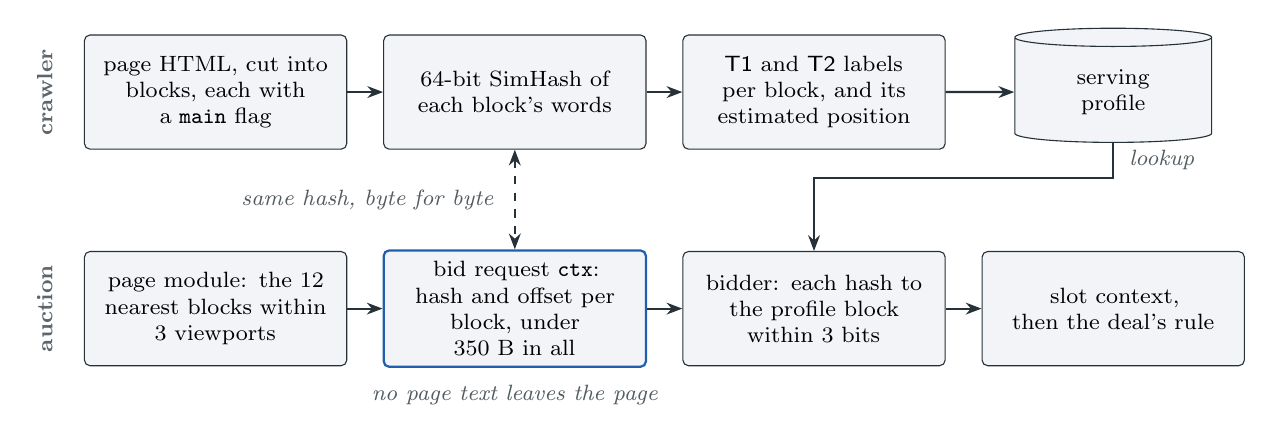
\begin{tikzpicture}[
  fstep/.style={box,text width=3.05cm,minimum height=1.45cm,font=\footnotesize},
  lane/.style={font=\footnotesize\bfseries,text=ink!75,rotate=90,anchor=south}]
  % Offline row: the crawler.
  \node[fstep] (html) at (1.75,0) {page HTML, cut into\\blocks, each with\\a \code{main} flag};
  \node[fstep] (sh) at (5.55,0) {64-bit SimHash of\\each block's words};
  \node[fstep] (lab) at (9.35,0) {\tier{1} and \tier{2} labels\\per block, and its\\estimated position};
  \node[store,minimum width=2.5cm,minimum height=1.45cm,font=\footnotesize] (st) at (13.15,0) {serving\\profile};
  \draw[arrow] (html) -- (sh);
  \draw[arrow] (sh) -- (lab);
  \draw[arrow] (lab) -- (st);
  % Online row: the browser, then the bidder.
  \node[fstep] (mod) at (1.75,-2.75) {page module: the 12\\nearest blocks within\\3 viewports};
  \node[fstep,draw=accent,thick] (wire) at (5.55,-2.75) {bid request \code{ctx}:\\hash and offset per\\block, under 350 B in all};
  \node[fstep] (match) at (9.35,-2.75) {bidder: each hash to\\the profile block\\within 3 bits};
  \node[fstep] (ctx) at (13.15,-2.75) {slot context,\\then the deal's rule};
  \draw[arrow] (mod) -- (wire);
  \draw[arrow] (wire) -- (match);
  \draw[arrow] (match) -- (ctx);
  \draw[arrow] (st.south) -- ++(0,-0.45) -| (match.north);
  \node[note,anchor=west] at ($(st.south)+(0.08,-0.22)$) {lookup};
  \draw[dashedarrow,{Stealth[length=2mm]}-{Stealth[length=2mm]}] (sh.south) -- (wire.north);
  \node[note,anchor=east] at (5.4,-1.375) {same hash, byte for byte};
  \node[note,below=1mm of wire.south] {no page text leaves the page};
  \node[lane] at (-0.2,0) {crawler};
  \node[lane] at (-0.2,-2.75) {auction};
\end{tikzpicture}
\caption{From the page module to the slot's context. Offline, the crawler labels
  each block and stores its SimHash in the serving profile. At auction time,
  the browser sends only hashes and offsets. The bidder joins them to the
  profile's blocks and computes the slot's context by
  \cref{eq:boundary-relevance,eq:boundary-suitability} with the format's
  geometry.}
\label{fig:boundary-flow}
\end{figure}

\subsection{Slot odds are priors}\label{sec:boundary-odds}

The lab ranks slots for a creative described in words. Each slot gets two
numbers. Fit is the chance that the creative suits the slot, given that the
slot is seen. Reach is the chance that the reader scrolls as far as the slot.
Their product is the slot's odds:
\begin{equation}\label{eq:boundary-odds}
\text{fit} = \sigma\bigl(12\,(\text{score} - 0.25)\bigr),\qquad
\text{reach} = e^{-y/6},\qquad
P = \text{fit} \times \text{reach},
\end{equation}
where score is the matcher's score on the slot's context (\cref{sec:serving}),
fit is $0$ when a hard rule blocks the creative, and $y$ is the slot's depth
in viewports from the top of the page. A slot 4.2 viewports down with a fit of
0.88 gets a reach of 0.50 and odds of 0.44. Slots go where the page's
template puts its ad containers. Without any container, a slot is tried after
each main paragraph, quote, caption, image or embed. A full-screen format gets
a single page-level slot.

\begin{figure}[t]
\centering
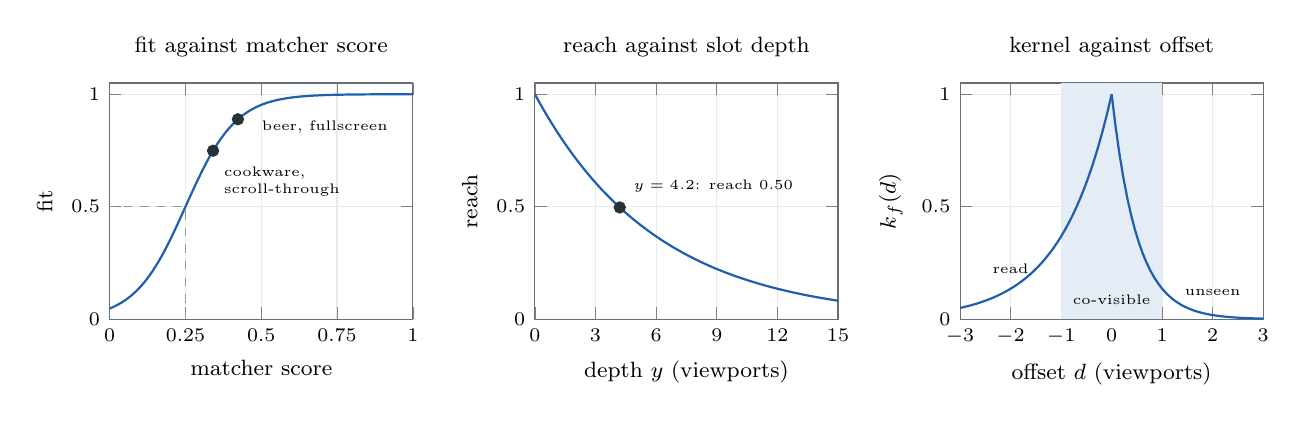
\begin{tikzpicture}
\begin{groupplot}[group style={group size=3 by 1,horizontal sep=1.55cm},
  scale only axis,width=3.85cm,height=3.0cm,
  tick label style={font=\scriptsize},label style={font=\footnotesize},
  title style={font=\footnotesize},axis line style={ink!70},
  every axis plot/.append style={thick},grid=major,grid style={ink!10}]
\nextgroupplot[title={fit against matcher score},xlabel={matcher score},
  ylabel={fit},xmin=0,xmax=1,ymin=0,ymax=1.05,xtick={0,0.25,0.5,0.75,1},
  xticklabels={0,0.25,0.5,0.75,1}]
  \addplot[accent,domain=0:1,samples=80] {1/(1+exp(-12*(x-0.25)))};
  \addplot[only marks,mark=*,mark size=1.8pt,ink,samples at={0.341,0.423}] {1/(1+exp(-12*(x-0.25)))};
  \node[font=\tiny,anchor=north west,align=left] at (axis cs:0.345,0.72) {cookware,\\scroll-through};
  \node[font=\tiny,anchor=west] at (axis cs:0.47,0.855) {beer, fullscreen};
  \draw[ink!50,dashed,thin] (axis cs:0.25,0) -- (axis cs:0.25,0.5) -- (axis cs:0,0.5);
\nextgroupplot[title={reach against slot depth},xlabel={depth $y$ (viewports)},
  ylabel={reach},xmin=0,xmax=15,ymin=0,ymax=1.05,xtick={0,3,6,9,12,15}]
  \addplot[accent,domain=0:15,samples=60] {exp(-x/6)};
  \addplot[only marks,mark=*,mark size=1.8pt,ink,samples at={4.2}] {exp(-x/6)};
  \node[font=\tiny,anchor=south west] at (axis cs:4.4,0.52) {$y=4.2$: reach 0.50};
\nextgroupplot[title={kernel against offset},xlabel={offset $d$ (viewports)},
  ylabel={$k_f(d)$},xmin=-3,xmax=3,ymin=0,ymax=1.05,xtick={-3,-2,-1,0,1,2,3}]
  \fill[accent!12] (axis cs:-1,0) rectangle (axis cs:1,1.05);
  \addplot[accent,domain=-3:0,samples=40] {exp(x)};
  \addplot[accent,domain=0:3,samples=40,forget plot] {exp(-2*x)};
  \node[font=\tiny,anchor=south] at (axis cs:0,0.02) {co-visible};
  \node[font=\tiny,anchor=south] at (axis cs:-2,0.16) {read};
  \node[font=\tiny,anchor=south] at (axis cs:2,0.06) {unseen};
\end{groupplot}
\end{tikzpicture}
\caption{The priors the lab uses, as plotted functions. Left: fit is a logistic
  of the matcher's score and crosses 0.5 at a score of 0.25; the dots are the
  two winners of \cref{tab:boundary-example}. Middle: reach decays with depth;
  the dot is the slot of the placement API's example. Right: the kernel of
  \cref{eq:boundary-kernel}, shared by every format today, falls twice as fast
  below the slot as above it. The shaded band is the co-visible window.}
\label{fig:boundary-priors}
\end{figure}

All of \cref{eq:boundary-odds} is hand-set. The logistic's slope and centre,
the six-viewport scroll decay, the page weights, the reaches and the width of
the co-visible window are priors chosen to be plausible, and each is marked as
a shortcut in the code. None has been fitted, because fitting needs engagement
data per slot, which we do not have yet. Fit should become the engagement
regression of \cref{sec:serving}, and reach should become measured scroll-depth
curves per site. Until then $P$ ranks slots within a page. It is not a
calibrated probability, and we do not report it as one.

\subsection{What is built and what is not}\label{sec:boundary-status}

As of 2026-11-11 the OCaml \code{Slot.context} computes
\cref{eq:boundary-relevance,eq:boundary-suitability}, and the served profile
carries up to 64 labelled blocks and the page's ad containers. The Go SDK's
\code{Profile.AtSlot} reproduces \code{Slot.context} on 2,000 fixture cases, in
1.8\,\textmu s with 23 allocations for five blocks, and
\code{Profile.SlotOfGPID} agrees with the OCaml side on 1,000. The page module
hashes as the crawler does. In the lab, the page view replays the archived
page with scripts off and draws block scores, slots, the kernel and the
co-visible window on it.

The rest is planned or unmeasured. No prior of \cref{tab:boundary-formats} or
\cref{eq:boundary-odds} is fitted, and the \code{sticky} and \code{fullscreen}
geometry has not been checked against each format's specification. The served
profile still estimates block positions. The module is not yet on publishers'
pages, and the bidder integration that would read \code{ctx} is open
(\cref{sec:serving}). Bid-time geometry also drifts from render time for
sticky and refreshing slots. We dropped three ideas for now: rendering one
page per template for desktop layouts, observing after the impression what was
co-visible, and using the previous page as context for interstitials, which
would bring in user history and consent obligations.

We plan to settle how far context reaches with data. The engagement model gets
two topic features per format, page-topic match and local-topic match, and
their fitted weights say how much nearby content matters. A script fits the
page feature at site grain on 30 days of delivery logs, because delivery is
reported per site; we report no result from it here. The local feature needs
slot geometry in the logs, which only the page module provides. The decisive
test is an A/B test of page context against slot context, crossed with format
(\cref{sec:protocol}). It has not run.

% 07-serving
\section{Serving and matching}\label{sec:serving}

The offline path leaves one compact profile per URL. At bid time the bidder
has to find that profile in one round trip, never wait for a crawl, decide
whether a deal or a creative may run there, say why, and rank what is left. We
split the work by language. The OCaml pipeline writes the profiles. The
bidder, written in Go, reads them through a small SDK. The rules therefore
exist twice, and both sides are checked against one set of fixtures that the
OCaml side writes.

\subsection{One key per page}\label{sec:serving-key}

A profile is found by its URL, so both sides must spell a URL the same way. Let
$\nu(u)$ be the bidder's own URL normalisation, the one it already applies
before its other per-URL lookups. The key of page $u$ is
\begin{equation}\label{eq:serving-key}
\kappa(u) = \texttt{contextual:} \,\|\, \operatorname{hex}\bigl(\operatorname{SHA\text{-}256}(\nu(u))\bigr).
\end{equation}
The OCaml side ports $\nu$ byte for byte from Go's \code{net/url} parser. It
drops the fragment, the scheme and any user information. It unescapes the
path, removes a leading \code{www.}\ from the host and one trailing slash from
the path, takes a fixed list of tracking parameters such as \code{utm\_source}
and \code{fbclid} out of the query, and removes a trailing \code{/amp}. The
host's case and port are kept. So
\code{https://www.example.com/news/article/amp?utm\_source=x\&fbclid=y\#top}
becomes \code{example.com/news/article}. A URL that Go refuses is refused
here too, so no profile is written under a key the bidder cannot compute. Any
difference would be a silent miss, so the port is tested on 111 cases written
by a Go implementation, 16 of them refused, and the Go SDK must recompute the
other 95 keys exactly.

\subsection{The serving profile}\label{sec:serving-profile}

The value under $\kappa(u)$ is a protobuf message, \code{PageProfile}, with a
30-day expiry (schema in \cref{app:wire}). It holds the \preset{rich} level's
labels, at most 20, highest score first; at most 20 keywords; the fetch time;
the preset's name; and the pipeline version, a hash of the taxonomy, lexicon,
models, calibration, thresholds and \tier{4} model, for logs and audits. The labels,
keywords, fetch time and preset take 252 bytes on average. For slot context
(\cref{sec:boundary}) the message also carries up to 64 labelled blocks, each
as its SimHash, its \code{main} flag, up to 8 labels and its estimated
position, and the page's ad containers. No block text is stored. The lab's full
profile, with every level, all evidence and the segments' text, is a separate
value of 9.3\,KB per page after zstd compression, which the bidder never
reads.

The labels obey one invariant, which saves the bidder a copy of the taxonomy.

\begin{definition}[Ancestor-closed profile]\label{def:serving-closed}
A label list $L$ with scores $s$ is \emph{ancestor-closed} when for every
$v \in L$ and every $u \in \operatorname{anc}(v)$, also $u \in L$ and
$s(u) \ge s(v)$.
\end{definition}

The cascade adds ancestors to every label (\cref{sec:cascade}), so served
profiles have this property. A rule on a node then needs no tree: ``Sports or
anything under it scores at least 0.5'' holds exactly when the id of Sports
itself is in the list with a score of at least 0.5. Checking one category
in the Go SDK is a scan of at most 20 labels.

\subsection{Backoff: page, section, site}\label{sec:serving-backoff}

A new article has no profile until the crawler reaches it, and most requests
miss while a crawl is young. So a page that misses inherits a profile from
where it lives. Write a normalised URL as $h/p_1/p_2/\dots$, with host $h$ and
the query left out. Its top section is $h/p_1$ (none when $p_1$ is empty) and
its site is $h$. Both have their own key,
\begin{equation}\label{eq:serving-section-key}
\kappa_s(q) = \texttt{contextual:section:} \,\|\, \operatorname{hex}\bigl(\operatorname{SHA\text{-}256}(q)\bigr),
\end{equation}
in a separate namespace, because a section's top page normalises to the same
string as the section. The bidder tries $\kappa(u)$, then the section's key,
then the site's (\cref{fig:serving-sequence}). We stop at the top section on
purpose: the bidder's store client may have no multi-key read, so each level
costs one more round trip on a miss.

A section's profile is the mean of its pages. Let $D_q$ be the pages saved
under prefix $q$, $n_q = |D_q|$, and $s_d(v)$ the served score of $v$ on page
$d$, with $s_d(v) = 0$ when $v$ is not among its served labels. The store keeps
the running sums $S_q(v) = \sum_{d \in D_q} s_d(v)$ and the count $n_q$. When
the crawler saves page $d$ with new scores $s'_d$, and $s_d$ are the scores it
added on its last crawl (all $0$ for a new page),
\begin{align}
S_q(v) &\leftarrow S_q(v) + s'_d(v) - s_d(v) \quad\text{for every } v \text{ in either list},\label{eq:serving-sums}\\
n_q &\leftarrow n_q + [\,d \text{ is new}\,],\nonumber\\
\bar{s}_q(v) &= S_q(v) / n_q, \quad\text{served once } n_q \ge 5.\label{eq:serving-mean}
\end{align}
A recrawled page therefore takes back what it added before, and the mean stays
the mean of each page's latest scores. One Lua script applies
\cref{eq:serving-sums} to the section and the site in a single atomic step,
deletes sums that fall below $10^{-6}$ and returns the hashes. The crawler then
writes each prefix with at least 5 pages as a \code{PageProfile}: its 20
highest means, no keywords, under $\kappa_s(q)$ with the same 30-day expiry.
The previous scores come from the page's summary in the store, so no second
copy of the profile is read.

\begin{proposition}\label{prop:serving-closed}
If every page's served labels are ancestor-closed, so are the section's means
in \cref{eq:serving-mean}, before the cut to the 20 highest.
\end{proposition}
\begin{proof}
Take $u \in \operatorname{anc}(v)$. On every page $s_d(u) \ge s_d(v)$: when $v$
is served this is \cref{def:serving-closed}, and otherwise $s_d(v) = 0$. Sum
over $D_q$ and divide by $n_q$.
\end{proof}

So \code{Rule.Check} reads a section profile as it reads a page's; the cut to
20 can only break this on a tie at the boundary. On the golden crawl, 383 pages
give 37 sections and sites with at least 5 pages. On the Pi cluster, adding
3,236 stored pages took 37 seconds and produced 1,318 prefixes, 242 of which
reached 5 pages after a run with synthetic traffic. Hubs such as home pages,
section fronts and live blogs change on almost every fetch, so the crawler
deletes their page key on purpose and the bidder backs off to their section,
which they keep feeding. Two limits remain. A page counts in its section until
it is recrawled, however old; a window or a decay would fix that if sections
drift. And URLs that start with a date give a year as their ``section''.

\begin{figure}[t]
\centering
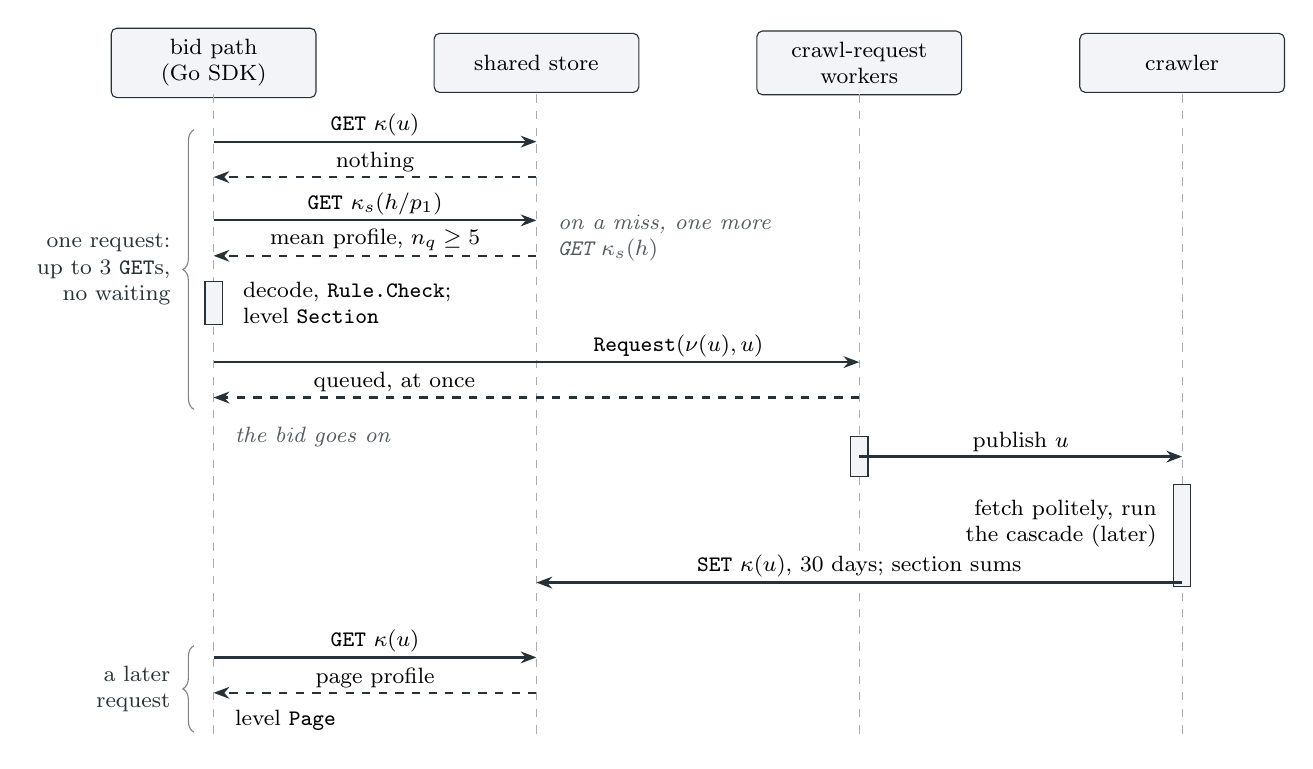
\begin{tikzpicture}[
  head/.style={box,minimum width=2.6cm,minimum height=0.75cm,font=\footnotesize},
  msg/.style={font=\footnotesize,above,inner sep=1.5pt,fill=white},
  act/.style={draw=ink,fill=soft,minimum width=0.22cm,inner sep=0pt},
  life/.style={draw=ink!40,dashed}]
  \foreach \x/\n/\t in {0/bid/{bid path\\(Go SDK)},4.1/st/{shared store},8.2/wk/{crawl-request\\workers},12.3/cr/{crawler}} {
    \node[head] (\n) at (\x,0) {\t};
    \draw[life] (\x,-0.4) -- (\x,-8.6);
  }
  % Miss on the page key.
  \draw[arrow] (0,-1.0) -- node[msg] {\code{GET} $\kappa(u)$} (4.1,-1.0);
  \draw[dashedarrow] (4.1,-1.45) -- node[msg] {nothing} (0,-1.45);
  % Section hit.
  \draw[arrow] (0,-2.0) -- node[msg] {\code{GET} $\kappa_s(h/p_1)$} (4.1,-2.0);
  \draw[dashedarrow] (4.1,-2.45) -- node[msg] {mean profile, $n_q \ge 5$} (0,-2.45);
  \node[note,anchor=west,align=left] at (4.25,-2.22) {on a miss, one more\\\code{GET} $\kappa_s(h)$};
  % Local work on the bid path.
  \node[act,minimum height=0.55cm] at (0,-3.05) {};
  \node[font=\footnotesize,anchor=west,align=left] at (0.25,-3.05) {decode, \code{Rule.Check};\\level \code{Section}};
  % Crawl request, never blocking.
  \draw[arrow] (0,-3.8) -- node[msg,pos=0.72] {\code{Request}$(\nu(u), u)$} (8.2,-3.8);
  \draw[dashedarrow] (8.2,-4.25) -- node[msg,pos=0.72] {queued, at once} (0,-4.25);
  \node[note,anchor=west] at (0.15,-4.75) {the bid goes on};
  \node[act,minimum height=0.5cm] at (8.2,-5.0) {};
  \draw[arrow] (8.2,-5.0) -- node[msg] {publish $u$} (12.3,-5.0);
  % The crawler, later.
  \node[act,minimum height=1.3cm] at (12.3,-6.0) {};
  \node[font=\footnotesize,anchor=east,align=right] at (12.1,-5.85) {fetch politely, run\\the cascade (later)};
  \draw[arrow] (12.3,-6.6) -- node[msg] {\code{SET} $\kappa(u)$, 30 days; section sums} (4.1,-6.6);
  % Next request for the same page.
  \draw[arrow] (0,-7.55) -- node[msg] {\code{GET} $\kappa(u)$} (4.1,-7.55);
  \draw[dashedarrow] (4.1,-8.0) -- node[msg] {page profile} (0,-8.0);
  \node[font=\footnotesize,anchor=west] at (0.15,-8.35) {level \code{Page}};
  % Braces.
  \draw[decorate,decoration={brace,amplitude=4pt,mirror},ink!60] (-0.25,-0.85) -- (-0.25,-4.4)
    node[midway,left=5pt,font=\footnotesize,align=right,text=ink] {one request:\\up to 3 \code{GET}s,\\no waiting};
  \draw[decorate,decoration={brace,amplitude=4pt,mirror},ink!60] (-0.25,-7.4) -- (-0.25,-8.5)
    node[midway,left=5pt,font=\footnotesize,align=right,text=ink] {a later\\request};
\end{tikzpicture}
\caption{A bid-time lookup for a page nobody has crawled yet. The page key
  misses, the top section's mean profile answers, and the deal's rule runs on
  it locally. The crawl request returns at once; a worker publishes it off the
  bid path, and a later request for the same page finds its own profile.}
\label{fig:serving-sequence}
\end{figure}

\subsection{Crawl requests on a miss}\label{sec:serving-crawl}

Every request that does not find its page's own profile asks the crawler for
it. The call must never slow the bid, so \code{CrawlRequests.Request} does only
a map lookup and a channel send. It first marks the normalised URL as asked;
a URL asked before returns \emph{already asked}. It then offers the page to a
bounded queue and returns \emph{queued}, or \emph{dropped} when the queue is
full or closed. A fixed pool of workers takes pages off the queue and
publishes each URL, one message per page, to a topic the crawler subscribes
to. A page that is dropped, or whose publish fails, is forgotten, so the next
miss asks again. The set of asked pages starts over at 100,000 entries; a
repeat then costs one message, which the crawler drops. The path from the SDK to the crawler was checked end to
end on an emulator of the message service, with its real client library. The
topic, the subscription and the permissions belong
to the bidder's infrastructure and are not set up yet.

\subsection{Hard rules, then a soft score}\label{sec:serving-rules}

Matching runs in two stages (\cref{tab:serving-pipeline}). Hard rules come
first, in a fixed order, and each refusal comes with a sentence a trader can
read. A label counts once its score is at least 0.5, a node counts together
with its descendants, and the reason names the deepest node that matched.
Blocks are none-of: blocking Sports also blocks Soccer. Suitability refuses a
creative that avoids Sensitive Topics when any node under that branch is on
the page. Targets are any-of, and a descendant counts, so targeting Food \&
Drink matches Cooking. When a campaign under-delivers, the
logged refusals say which rule starves it.

\begin{table}[t]
\centering
\caption{The matcher's stages (\code{Matcher.refusal} and \code{Matcher.score}
  in \code{src/lib/matcher.ml}), in order, with the reasons the test suite
  prints. The Go SDK ports the three hard rules as \code{Rule.Check}; the soft
  score stays in OCaml.}
\label{tab:serving-pipeline}
\small
\begin{tabularx}{\linewidth}{@{}l >{\raggedright\arraybackslash}p{4.1cm} >{\raggedright\arraybackslash}X l@{}}
\toprule
Stage & Passes when & Reason printed when it decides & Go verdict\\
\midrule
1. blocks & no blocked node on the page & advertiser blocks Sports; page is Sports > Soccer (0.92) & blocked\\
2. suitability & the creative accepts Sensitive Topics, or none is on the page & brand suitability: page is Sensitive Topics > Crime \& Harmful Acts\dots\ (0.89) & unsuitable\\
3. targets & no targets, or one is on the page & no targeted category on page & off-target\\
4. soft score & stages 1--3 passed & topic Sports > Soccer $\sim$ Sports > Soccer (0.83); keywords: premier league & not ported\\
\bottomrule
\end{tabularx}
\end{table}

Creatives that pass get a score from three named features. The
first is topical. Let page $d$ carry labels $u$ with scores $s_u$ and creative
$c$ carry labels $w$ with scores $t_w$, both in the same \iab{} label space. With
$\operatorname{depth}(v) = |\operatorname{anc}(v)|$, so that a root has depth
1, the Wu--Palmer similarity of two nodes is
\begin{equation}\label{eq:serving-wup}
\operatorname{wp}(u, w) = \frac{2\,\operatorname{depth}(\operatorname{lca}(u, w))}{\operatorname{depth}(u) + \operatorname{depth}(w)}
 = \frac{2\,|\operatorname{anc}(u) \cap \operatorname{anc}(w)|}{|\operatorname{anc}(u)| + |\operatorname{anc}(w)|},
\end{equation}
and $0$ when $u$ and $w$ sit under different roots (\cref{fig:serving-wup}).
It is 1 for the same node, $2/3$ for a root and its child, and $1/2$ for two
children of a root. The topic feature takes the best pair,
\begin{equation}\label{eq:serving-topic}
\operatorname{topic}(d, c) = \max_{u, w}\; s_u\, t_w\, \operatorname{wp}(u, w),
\end{equation}
and reports that pair as its reason. This is the taxonomy score of
\citet{broder2007semantic}, which backs off through the lowest common ancestor
in the same way. The keyword feature is the share of the creative's keywords
$K_c$ found among the page's $K_d$, after both pass through the same text
normaliser: $\operatorname{kw}(d, c) = |K_c \cap K_d| / |K_c|$, and $0$ when
$K_c$ is empty. Requiring the ad's keywords on the page lifted average
precision by 60\% over plain cosine matching in \citet{ribeironeto2005impedance}. The lift feature
is $\operatorname{lift}(d, c) = \max_u s_u\, A(\pi_c, u)$, where $\pi_c$ is the
creative's product category and $A$ a table of learned affinities between
product and page categories. Because $A$ is keyed by product, a new creative
inherits what its category has already taught, and beer can score on a sports
page without any topical overlap. The score is
\begin{equation}\label{eq:serving-score}
\operatorname{score}(d, c) = 0.6\,\operatorname{topic}(d, c) + 0.25\,\operatorname{kw}(d, c) + 0.15\,\operatorname{lift}(d, c).
\end{equation}
On a football match report the test suite gives boots 0.621, from the pair
Soccer $\sim$ Soccer (0.83) and the keyword ``premier league''; beer 0.083,
from a test lift of Beer on Sports; an electric car blocked by its
advertiser's block on Sports; and cookware off-target.

\begin{figure}[t]
\centering
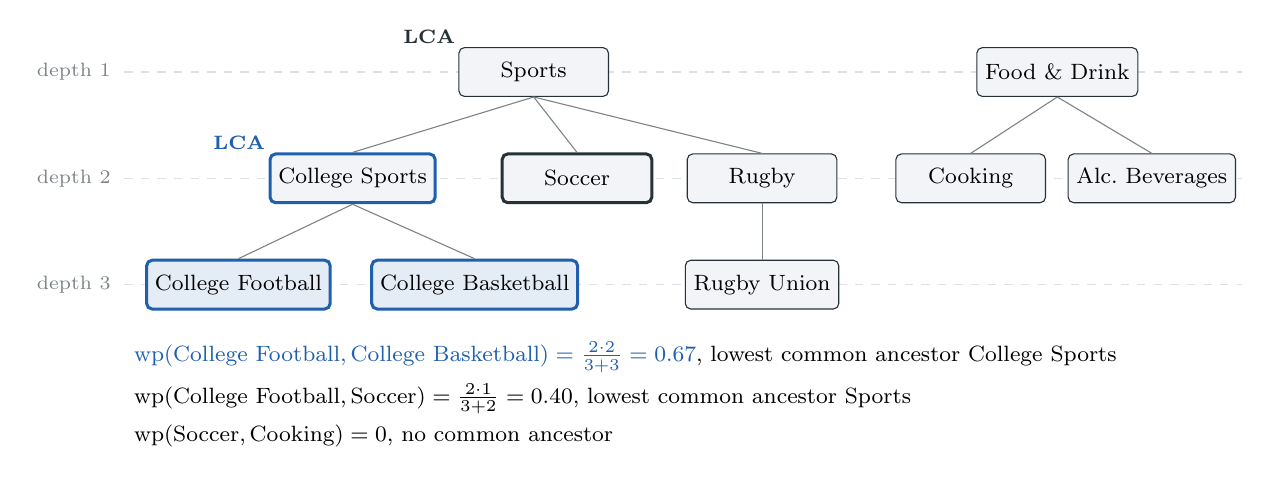
\begin{tikzpicture}[
  tn/.style={box,font=\footnotesize,minimum width=1.9cm,minimum height=0.62cm,inner sep=3pt},
  hl/.style={tn,draw=accent,line width=1.1pt,fill=accent!12},
  dk/.style={tn,draw=ink,line width=1.1pt},
  tag/.style={font=\scriptsize\bfseries,inner sep=1pt},
  edge/.style={draw=ink!60}]
  \foreach \y/\t in {0/depth 1,-1.35/depth 2,-2.7/depth 3} {
    \draw[ink!15,dashed] (-2.0,\y) -- (12.2,\y);
    \node[font=\scriptsize,text=ink!60,anchor=east] at (-2.05,\y) {\t};
  }
  \node[tn] (sp) at (3.2,0) {Sports};
  \node[tn,draw=accent,line width=1.1pt] (cs) at (0.9,-1.35) {College Sports};
  \node[dk] (so) at (3.75,-1.35) {Soccer};
  \node[tn] (ru) at (6.1,-1.35) {Rugby};
  \node[hl] (cf) at (-0.55,-2.7) {College Football};
  \node[hl] (cb) at (2.45,-2.7) {College Basketball};
  \node[tn] (rl) at (6.1,-2.7) {Rugby Union};
  \node[tn] (fd) at (9.85,0) {Food \& Drink};
  \node[tn] (co) at (8.75,-1.35) {Cooking};
  \node[tn] (ab) at (11.05,-1.35) {Alc.\ Beverages};
  \foreach \a/\b in {sp/cs,sp/so,sp/ru,cs/cf,cs/cb,ru/rl,fd/co,fd/ab} \draw[edge] (\a.south) -- (\b.north);
  \node[tag,text=accent,anchor=south east] at (cs.north west) {LCA};
  \node[tag,text=ink,anchor=south east] at (sp.north west) {LCA};
  \node[font=\footnotesize,align=left,anchor=north west] at (-2.0,-3.3) {%
    \textcolor{accent}{$\operatorname{wp}(\text{College Football}, \text{College Basketball}) = \tfrac{2\cdot 2}{3+3} = 0.67$},
      lowest common ancestor College Sports\\[3pt]
    $\operatorname{wp}(\text{College Football}, \text{Soccer}) = \tfrac{2\cdot 1}{3+2} = 0.40$,
      lowest common ancestor Sports\\[3pt]
    $\operatorname{wp}(\text{Soccer}, \text{Cooking}) = 0$, no common ancestor};
\end{tikzpicture}
\caption{Wu--Palmer similarity on two branches of \iab. Two leaves under the
  same parent (filled blue) meet at College Sports and score 0.67. College
  Football and Soccer (dark outline) meet only at the root and score 0.40.
  Nodes under different roots score 0, so a topic match never crosses from
  Sports to Food \& Drink.}
\label{fig:serving-wup}
\end{figure}

The weights 0.6, 0.25 and 0.15 are set by hand. They are a placeholder for a
learned model, marked as a shortcut in the code, and we make no claim that
they are right. The plan is a logistic regression on engagement over the same
named features with format and device crosses, as
\citet{chakrabarti2008contextual} did for clicks, so that the weights stay
readable as logits. A contextual bandit over the same features
\citep{li2010contextual} would then explore among eligible creatives, with
propensities logged for offline evaluation, and a floor below which the bidder
does not force relevance and falls back to its non-contextual bid
\citep{broder2008swing}. The lift table is empty today, so lift is 0 in
every score today. The creative side is also thin: a creative comes from a text
prompt labelled by \tier{1} and \tier{2}, not yet from its ad copy and landing
page, and product categories are not loaded.

\subsection{Curated deals: placement list or context}\label{sec:serving-deals}

The first use is curated deals. A deal takes a request whose placement is on
its list, \emph{or} whose page matches its context. If deal filters are ANDed,
a separate context filter could only shrink supply, so the OR belongs inside
the placement check:
\begin{lstlisting}
func placementOK(deal *Deal, req *BidRequest) bool {
    if deal.Placements.Contains(req.PlacementID) {
        return true
    }
    return deal.ContextRule != nil && req.ContextualLevel != contextual.NotFound &&
        deal.ContextRule.Check(&req.Contextual).Verdict == contextual.Eligible
}
\end{lstlisting}
A deal's context is a \code{Rule}: its targets, blocks, Sensitive Topics choice
and a minimum score, 0.5 by default. A page with no profile at any level is not
eligible, as keyword targeting treats a request without keywords. When the
request names the blocks around its slot, the rule can run on the slot's
context from \code{Profile.AtSlot} instead of the page's
(\cref{sec:boundary}). The bidder integration is written as a guide, not
deployed. Its first step is a shadow mode that only counts, per deal, the
requests context would add. A per-deal minimum score that falls when a deal is
behind pace and rises when it is ahead is planned, as are per-bid logs of each
decision.

\subsection{An allocation-free reader}\label{sec:serving-reader}

A bidder decodes a profile on every request, so the decoder must not allocate.
\code{Profile.Decode} walks the protobuf wire format by hand. It reuses the
profile's slices, so a pooled profile decodes in place. Label ids are not
copied: they point into the input buffer, which must not change while the
profile is in use. Every block's labels share one backing array. Fields the
decoder does not know are skipped, so a writer can add fields without breaking
deployed readers. The tests assert zero allocations for decoding a profile
with blocks and for a decode followed by \code{Rule.Check}.
\Cref{tab:serving-sdk} lists the calls, their cost and the fixtures that pin
each one to the OCaml side.

\begin{table}[t]
\centering
\caption{The Go SDK's calls (\code{sdks/go/contextual}). Costs are Go
  benchmarks on an Apple M4. Fixtures are written by the OCaml side, so both
  implementations answer the same cases.}
\label{tab:serving-sdk}
\small
\begin{tabularx}{\linewidth}{@{}l >{\raggedright\arraybackslash}X l l@{}}
\toprule
Call & What it does & Cost per call & Checked against\\
\midrule
\code{Key} & the page's key, \cref{eq:serving-key} & 83\,ns, 2 allocations & 95 URLs\\
\code{Sections}, \code{SectionKey} & prefixes and their keys, \cref{eq:serving-section-key} & & the same 95 URLs\\
\code{LookupWithBackoff} & page, then section, then site & one \code{GET} per level & unit tests\\
\code{Profile.Decode} & protobuf into a reused profile & 83\,ns, no allocation & every fixture\\
\code{Rule.Check} & a deal's rule and its reason & 9\,ns, no allocation & 3,000 profiles\\
\code{Profile.AtSlot} & the slot's context (\cref{sec:boundary}) & 1.8\,\textmu s, 23 allocations & 2,000 cases\\
\code{Profile.SlotOfGPID} & the slot's blocks from a GPID & & 1,000 cases\\
\code{CrawlRequests.Request} & a crawl request that never blocks & a map lookup, a send & unit tests\\
\bottomrule
\end{tabularx}
\end{table}

The 3,000 rule fixtures are profiles built as the cascade builds them, with
ancestors added and scores rounded to 32-bit floats as the wire carries them,
each paired with a random deal rule and the OCaml matcher's verdict. The 2,000
slot fixtures pair a profile with the \code{ctx} of a bid request. Most of its
hashes copy one of the profile's blocks with up to 5 bits flipped and the rest
are random, so both sides of the 3-bit threshold are exercised. \code{AtSlot} must match \code{Slot.context}
to within $10^{-5}$ on every label. The fixtures are regenerated after any
change to the matcher, the label order or the profile format.

% 08-implementation
\section{Implementation}\label{sec:impl}

\sys{} is written in OCaml~5 and built with dune; the source is at \repo. The numerical work runs in C: two neural models on a vendored copy of ggml, an HTML5 parser and Google's robots.txt matcher, each behind a small adapter. A Go library reads the serving profiles inside the bidder, and a Prebid.js module writes the slot context into the bid request. This section explains how the pieces fit, what the C code bought, how the fleet shares state, and what the system does on three Raspberry Pi boards.

\subsection{Processes}\label{sec:impl-processes}

Three kinds of process share one key-value store (\cref{fig:impl-layout}). Crawl daemons claim pages, fetch them, run the cascade and write profiles. Online servers read new profiles every three seconds, score slots for a creative described in words and serve the lab's front end. Valkey holds everything they share; \cref{tab:impl-keys} lists the key families. Any number of crawlers and online servers can run: none keeps state another needs.

\begin{figure}[t]
\centering
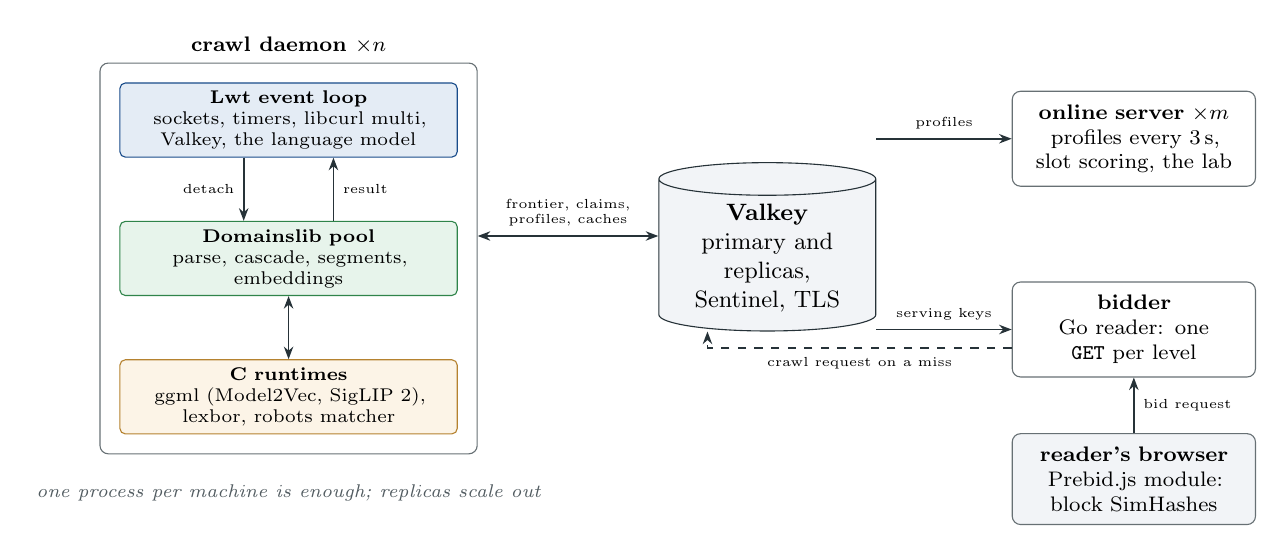
\begin{tikzpicture}[x=1cm,y=1cm,font=\footnotesize,scale=0.95,transform shape]
\tikzset{
  iproc/.style={draw=ink!70, rounded corners=3pt, fill=white, inner sep=5pt},
  ilane/.style={draw=#1!80!black, fill=#1!12, rounded corners=2pt, align=center, inner sep=3pt, font=\scriptsize, minimum height=6mm},
  ilink/.style={-{Stealth[length=1.6mm]}, semithick, draw=ink},
  ilink2/.style={{Stealth[length=1.6mm]}-{Stealth[length=1.6mm]}, semithick, draw=ink},
  inote/.style={note, font=\scriptsize\itshape},
}
% crawler internals
\node[ilane=accent, text width=4.3cm] (loop) at (0,2.45) {\textbf{Lwt event loop}\\sockets, timers, libcurl multi,\\Valkey, the language model};
\node[ilane=ttwo, text width=4.3cm] (pool) at (0,0.6) {\textbf{Domainslib pool}\\parse, cascade, segments,\\embeddings};
\node[ilane=tthree, text width=4.3cm] (cstub) at (0,-1.25) {\textbf{C runtimes}\\ggml (Model2Vec, SigLIP~2),\\lexbor, robots matcher};
\draw[ilink] ([xshift=-6mm]loop.south) -- node[left, font=\tiny] {detach} ([xshift=-6mm]pool.north);
\draw[ilink] ([xshift=6mm]pool.north) -- node[right, font=\tiny] {result} ([xshift=6mm]loop.south);
\draw[ilink2] (pool.south) -- (cstub.north);
\node[iproc, fill=none, fit=(loop)(pool)(cstub), inner sep=7pt] (crawler) {};
\node[font=\footnotesize\bfseries, anchor=south] at (crawler.north) {crawl daemon $\times n$};

% valkey
\node[store, minimum width=2.9cm, minimum height=2.1cm, align=center] (vk) at (6.4,0.6) {\textbf{Valkey}\\primary and\\replicas,\\Sentinel, TLS};
\draw[ilink2] (crawler.east |- 0.9,0.9) -- node[above, font=\tiny, align=center] {frontier, claims,\\profiles, caches} (vk.west |- 0.9,0.9);

% online
\node[iproc, align=center, text width=2.9cm] (online) at (11.3,2.2) {\textbf{online server $\times m$}\\profiles every 3\,s,\\slot scoring, the lab};
\node[iproc, align=center, text width=2.9cm] (bidder) at (11.3,-0.35) {\textbf{bidder}\\Go reader: one\\\code{GET} per level};
\draw[ilink] (vk.east |- online.west) -- node[above, font=\tiny] {profiles} (online.west);
\draw[ilink] (vk.east |- bidder.west) -- node[above, font=\tiny] {serving keys} (bidder.west);
\node[iproc, align=center, text width=2.9cm, fill=soft] (page) at (11.3,-2.35) {\textbf{reader's browser}\\Prebid.js module:\\block SimHashes};
\draw[ilink] (page.north) -- node[right, font=\tiny] {bid request} (bidder.south);
\draw[ilink, dashed] ([yshift=-2.5mm]bidder.west) -| node[pos=0.25, below, font=\tiny] {crawl request on a miss} ([xshift=-8mm]vk.south);
\node[inote, anchor=north] at (0,-2.3) {one process per machine is enough; replicas scale out};
\end{tikzpicture}
\caption{Processes and what they share. Inside a crawl daemon, the event loop owns every socket and the pool does every CPU-heavy step; work crosses between them only through \code{detach}. Crawl daemons and online servers keep no state of their own, so any number can run. The bidder reads serving keys and, on a miss, asks for a crawl.}
\label{fig:impl-layout}
\end{figure}

\subsection{I/O on one domain, CPU on the others}\label{sec:impl-concurrency}

OCaml~5 runs code in parallel on several domains. We use two libraries, each for what it is good at. Lwt owns the main domain: sockets, timers, libcurl's multi interface for fetches, the Valkey client and calls to the language model. A Domainslib pool runs everything that needs a CPU: parsing, the cascade, segment labels, embeddings. The bridge between them is one function, \code{detach pool f x}. It posts \code{f x} to the pool and returns an Lwt promise. When the worker finishes, it hands the result back through Lwt's notification pipe, the one thread-safe way into the event loop.

Inside a job, work fans out again. \code{Web.parallel pool} gives the engine a map that runs Domainslib's \code{parallel\_for}, over a page's segments or, in the online server, over every crawled page when it scores a creative's reach. This nesting is why we did not use \code{lwt\_domain}: it makes the pool's type abstract, and a nested \code{parallel\_for} needs the pool itself. One rule prevents a class of crashes: no lazy value is shared across domains. A lazy value forced from two domains at once raises an exception. So prototypes are built eagerly at start, and each page's lazy content is forced once, in one job, before anything runs on it in parallel.

The cascade is a pure function, but two of its tiers need the network. \Cref{alg:cascade-phases} splits a page into phases so that a worker never waits on a socket: the pool runs every level, the loop fetches images and calls the model, the pool runs again. A slow provider holds a promise on the event loop, not a CPU.

\subsection{C where it pays}\label{sec:impl-c}

Every C dependency is vendored and wrapped in a flat adapter: a few functions taking and returning plain arrays and strings, so the OCaml side never walks C structures. Each replaced an OCaml version, and each was checked against a reference implementation before it was kept. \Cref{fig:impl-speedups} gives the speedups.

\paragraph{Model2Vec on ggml.} Model2Vec turns a sentence into the mean of static token embeddings distilled from a sentence transformer \citep{tulkens2024model2vec}. The models are converted to GGUF and run on ggml, which does the matrix products with SIMD. ggml has no tokenizer, so we wrote ours in C: ports of the WordPiece and Unigram paths of model2vec-rs, plus Hugging Face's SentencePiece character-map normaliser. On 1,133,527 texts per model they give exactly Hugging Face's token ids; 722 synthetic texts per model stay in the test suite. The real gain is in the similarity step. It was 704 dot products per text over OCaml lists; it is now one matrix multiply per page. A whole profile, all presets and segment labels without \tier{4}, takes 8.5\,ms instead of 56.3\,ms on English pages and 19.7\,ms instead of 103.3\,ms in other languages, on the larger multilingual model.

\paragraph{SigLIP~2 on ggml.} The image tier runs SigLIP~2's vision tower \citep{tschannen2025siglip}, with weights quantised to Q8\_0: 100\,MB against 186\,MB in half precision. On our test images the embeddings agree with Hugging Face's to a cosine of 0.995 or better, and the zero-shot rankings are the same. Images are decoded by the system's libjpeg-turbo, libpng and libwebp rather than a single-header decoder whose author warns it is not meant for untrusted files; web images are untrusted input. On a laptop core an image takes 247\,ms at the model's default of 256 patches. A Raspberry Pi~4 core lacks the dot-product instructions of ggml's fast integer kernels, which gave 2.1 to 2.5 times on the laptop. There an image takes 3.46\,s on one thread at 128 patches, 0.94\,s on four. The crawler uses one thread per image and several images at once.

\paragraph{lexbor.} The HTML5 parser replaced a tolerant tag scanner: tokens come out 3.3 times faster (141 to 480\,MB/s), and tokens plus extraction 2.6 times faster, about 1.4\,ms a page. A third of that time is now building OCaml values, which is not worth moving to C while classification costs far more.

\paragraph{robots.txt.} Google's matcher runs through an adapter that parses a file once and replays only the rules that apply to us (\cref{sec:crawl-robots}). Two fixes inside the vendored code mattered most: a container that allocated and zero-filled memory for every rule tested, and user-agent matching repeated on every check.

\begin{figure}[t]
\centering
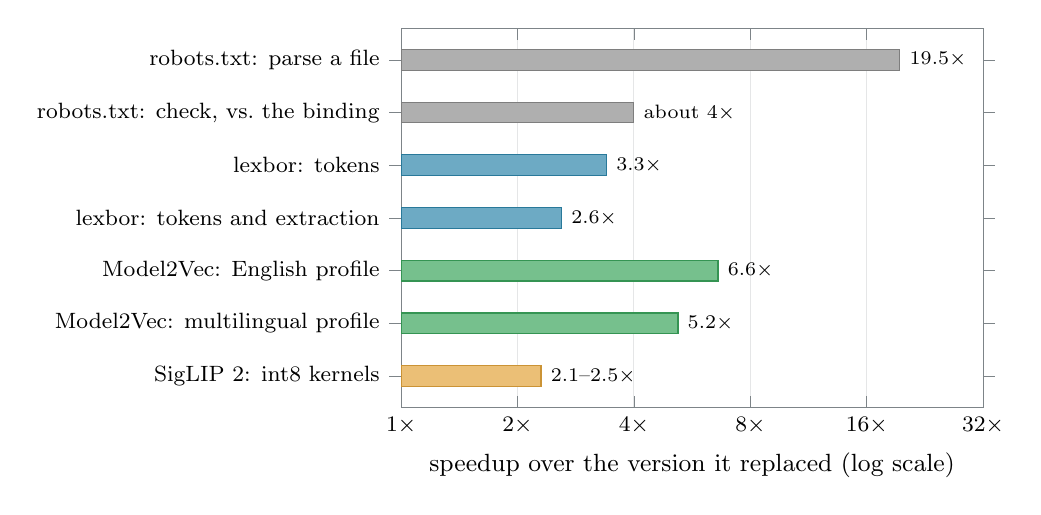
\begin{tikzpicture}
\begin{axis}[
  xbar, bar shift=0pt, width=0.74\linewidth, height=6.4cm,
  xmode=log, log basis x=2, xmin=1, xmax=32,
  xtick={1,2,4,8,16,32}, xticklabels={1$\times$,2$\times$,4$\times$,8$\times$,16$\times$,32$\times$},
  ytick={0,1,2,3,4,5,6}, y dir=reverse,
  yticklabels={
    {robots.txt: parse a file},
    {robots.txt: check, vs.\ the binding},
    {lexbor: tokens},
    {lexbor: tokens and extraction},
    {Model2Vec: English profile},
    {Model2Vec: multilingual profile},
    {SigLIP~2: int8 kernels},
  },
  yticklabel style={font=\footnotesize, align=right},
  xlabel={speedup over the version it replaced (log scale)},
  label style={font=\small}, ticklabel style={font=\footnotesize},
  bar width=7.5pt, enlarge y limits=0.1,
  axis line style={ink!60}, tick style={ink!60},
  xmajorgrids, grid style={ink!12},
  nodes near coords, nodes near coords style={font=\scriptsize, anchor=west},
  point meta=explicit symbolic,
]
\addplot[fill=tzero!70, draw=tzero!90!black] coordinates {(19.5,0) [19.5$\times$]};
\addplot[fill=tzero!70, draw=tzero!90!black] coordinates {(4,1) [about 4$\times$]};
\addplot[fill=tone!70, draw=tone!90!black] coordinates {(3.4,2) [3.3$\times$]};
\addplot[fill=tone!70, draw=tone!90!black] coordinates {(2.6,3) [2.6$\times$]};
\addplot[fill=ttwo!70, draw=ttwo!90!black] coordinates {(6.6,4) [6.6$\times$]};
\addplot[fill=ttwo!70, draw=ttwo!90!black] coordinates {(5.2,5) [5.2$\times$]};
\addplot[fill=tthree!70, draw=tthree!90!black] coordinates {(2.3,6) [2.1--2.5$\times$]};
\end{axis}
\end{tikzpicture}
\caption{What each C runtime bought, against the version it replaced: the pure OCaml robots.txt parser (parse) and the published binding (check), our OCaml tag scanner, Model2Vec in OCaml, and ggml's generic kernels for SigLIP~2 on a laptop core. Each was kept only after matching a reference implementation exactly or to a fixed tolerance.}
\label{fig:impl-speedups}
\end{figure}

\subsection{Shared state}\label{sec:impl-state}

\begin{table}[t]
\centering\small
\caption{Key families in the shared store and what each makes possible. Every step that touches more than one key runs as one Lua script.}
\label{tab:impl-keys}
\begin{tabularx}{\linewidth}{@{}>{\raggedright\arraybackslash}p{3.7cm}>{\raggedright\arraybackslash}X@{}}
\toprule
Keys & What they hold, and why \\
\midrule
frontier per origin; due origins; seen-set; claims & the queue of \cref{sec:crawl-frontier}: busiest first, one request at a time per site, each URL queued once in the fleet, dead crawlers' claims taken back \\
robots.txt and licences per origin & one fetch serves every replica, for 24 hours or the licence's maximum age \\
stored profiles (zstd JSON) and their index & every level, label, evidence record and block; the online servers reload what changed \\
serving profiles, per page and per section & the protobuf the bidder reads, 30 days (\cref{sec:serving}) \\
section and site sums & running sums of label scores per section and site, kept on every save \\
refresh state and schedule; bid requests per page & validators, SimHash, publication time, unchanged count; when to fetch next \\
image embeddings & one SigLIP~2 embedding per image URL and patch budget, 30 days \\
archive index; slot positions per template & where each page's WARC record is; ad positions learned per template \\
stats, recent events, replicas & the same status from any replica: what each crawled, \tier{4} calls and spend \\
\bottomrule
\end{tabularx}
\end{table}

The store runs as a primary and two replicas with Sentinel, over TLS with a password, each Sentinel on its own board. When the primary has been unreachable for 5 seconds, two Sentinels agree and promote a replica; the crawlers and online servers follow the new primary when a connection breaks or the server answers \code{READONLY}. The store uses append-only persistence and never evicts, so the frontier is never lost to memory pressure. With sections, refresh state and image embeddings, it grew from 45 to 60\,MB on the cluster's data.

One failure taught us something about high availability on small clusters. Sentinel rewrites its configuration on every failover, with the primary and its epoch, and that file lived in an ephemeral volume. After a full shutdown no Sentinel knew the primary, so every pod fell back to the first one. When that pod's node had stopped first, its stale copy became the primary and the others resynchronised from it: in a reproduction on a local cluster, all 1,000 keys written after it stopped were lost, on every node, while the append-only files were intact. The fix keeps each Sentinel's configuration on the data volume and, when no Sentinel answers at start, takes the primary its own Sentinel last knew. A stale primary that comes back alone is demoted within about 30 seconds.

\subsection{The pipeline version}\label{sec:impl-version}

A profile is only reproducible if we know what produced it. Every profile carries a pipeline version: 16 hexadecimal digits of a SHA-256 over the taxonomy, lexicon and model files byte for byte, the calibration constants, the per-language tunings, the presets, the image settings and \tier{4}'s model. The refresh test of \cref{eq:crawl-unchanged} uses it: a page whose text did not move is reclassified anyway when the version did. Code is not hashed. A change to the code that moves labels bumps a constant by hand, since hashing the binary would reclassify every page on every build.

\subsection{Three Raspberry Pis}\label{sec:impl-pi}

The lab runs on three Raspberry Pi~4 boards with 8\,GB each, under k3s: three crawl daemons with four workers each, two online servers and the three Valkey pods. Images are built natively for 64-bit ARM on a laptop and pulled from a registry inside the cluster. On 3,198 pages over 274 hosts, with \tier{4} off and images at 128 patches, the cluster crawled 1.9 pages a second end to end, about 160,000 a day, and stored 78\% of them; the rest were refused by HTTP 403 or robots.txt. The cascade, not the network, sets that rate: the boards ran at about three of their four cores. That is the order of the head of the traffic. The busy head is a small fraction of all pages, only a small share of new pages become busy (\cref{sec:crawl-which}), and a refresh that finds a page unchanged costs a fetch, not a classification. Every page a bidder sees, millions a day, is far out of reach of three boards; the value budget of \cref{eq:cascade-budget} is what keeps the tail cheap on any hardware.

The online servers load every profile they serve into memory, labels and evidence included. On 3,236 profiles that took about a gigabyte, and a one-gigabyte limit killed them; the lab now asks for two. The bidder does not have this problem: it reads one compact serving profile per lookup.

\subsection{Tests that pin behaviour}\label{sec:impl-tests}

Each C runtime is tested against its reference: tokenizer ids against Hugging Face, image embeddings against Hugging Face to a cosine tolerance, robots.txt against Google's one-shot matcher. Behaviour that two languages must share is pinned by fixtures that the OCaml side writes and the other side reads: 3,000 cases of the deal rule for the Go reader, 2,000 slot contexts, SimHash values in five languages for the Prebid module and the Go reader. The test suite also asserts end-to-end scenarios of the matcher, such as a crime headline in a co-visible widget blocking every creative on an otherwise safe food page. A failing test stops the container build.

% 09-evaluation
\section{Evaluation}\label{sec:eval}

We evaluate three things. How good are the labels, at each depth and against what they cost? Which language model should run \tier{4}? And would context change what buyers do, measured offline on an exchange's request logs? Throughput and freshness on real hardware are in \cref{sec:impl-pi,sec:crawl-refresh}.

\subsection{The golden set}\label{sec:eval-golden}

\paragraph{Pages.} We drew the golden sample from 25 of the busiest publishers on the exchange over one week, 20 pages each, drawn without replacement with probability proportional to impressions, so busy pages are more likely to appear. The draw hashes each URL, so it can be repeated. The sampled URLs and gold labels come from the exchange's traffic and are not published; the repository holds a made-up pair of files in the same format. Of the 469 pages, 383 could be crawled and stored; the other 86 answered with HTTP 403 or were disallowed by robots.txt. Four of the 25 publishers gave us nothing at all: some publishers refuse unknown crawlers. The stored pages follow the exchange's supply, not the web's: 112 are in Italian, 76 in French, 27 in German, 164 in English and 4 in other languages. Homepages are a large share of it, since they carry many impressions.

\paragraph{Labels.} The pages were crawled at \preset{deep}, with \tier{4} on, and then judged. We did not have readers of every language at hand, so an LLM did the judging, in two passes, and every judgement stays open to correction in the lab. In the first pass, a model (DeepSeek V4.1 Flash) saw exactly what a human judge sees in the lab: the top 12 labels of every level with their scores and evidence, and the full taxonomy to add what every level missed. It cost \$0.30 for 383 pages. In the second pass the same model re-judged the Italian and French pages while reading their text, up to 4,000 characters, which cost \$0.26. The two passes agree at \hF{} 0.798, and 124 of 188 pages came out identical. We adopted the second pass for the 176 article pages and kept the first for the 12 homepages, where reading every teaser added up to 70 labels a page. Ancestors are removed from each judgement, since the metric adds them back. The gold has 1,173 labels, 3.1 a page.

This is the weakest part of the evaluation, and we say so plainly. An LLM's labels are not ground truth, and \tier{4} is itself an LLM, so its scores below partly measure agreement between two models. A human check of 50 pages is the next step (\cref{sec:discussion}).

\paragraph{Metric.} Labels form a hierarchy, and a page judged Soccer that we label Sports is half right, not wrong. We use hierarchical precision and recall \citep{kiritchenko2006learning}: both the predicted set $\hat{Y}_d$ (labels served, score $\ge 0.5$) and the gold set $Y_d$ are closed under ancestors, then compared, micro-averaged over pages:
\begin{equation}\label{eq:eval-hprf}
  \hP = \frac{\sum_d |\operatorname{cl}(\hat{Y}_d) \cap \operatorname{cl}(Y_d)|}{\sum_d |\operatorname{cl}(\hat{Y}_d)|},
  \qquad
  \hR = \frac{\sum_d |\operatorname{cl}(\hat{Y}_d) \cap \operatorname{cl}(Y_d)|}{\sum_d |\operatorname{cl}(Y_d)|},
  \qquad
  \hF = \frac{2\,\hP\,\hR}{\hP + \hR}.
\end{equation}

\subsection{Label quality against depth}\label{sec:eval-quality}

\Cref{fig:eval-quality} and \cref{tab:eval-quality} compare what the levels served at crawl time, with the hand-set calibration, with what they serve now. The hand-set \tier{2} was badly overconfident: \preset{standard} served labels at a precision of 0.097, so nine served labels in ten were wrong, and recall was high only because almost everything was served. Calibration alone, before any change of threshold, raises \preset{standard}'s precision to 0.448 and its \hF{} from 0.171 to 0.373. \preset{rich} without \tier{4} gains the same way.

\begin{table}[t]
\centering\small
\caption{Served labels against the golden set. ``Stored'' is what the profiles served at crawl time, with the hand-set calibration and \tier{4} at \preset{deep}. ``Today'' reruns \tier{0}--\tier{3} offline on the same pages with the fitted calibration. The last row is \preset{rich} with the per-language tunings, where pages that do not settle take \tier{4}'s answer.}
\label{tab:eval-quality}
\begin{tabular}{@{}llccccc@{}}
\toprule
Level & Configuration & \hP & \hR & \hF & settled & \tier{4} \\
\midrule
\preset{zero\_fetch} & stored & 1.000 & 0.015 & 0.030 & 0\% & -- \\
\preset{standard} & stored, hand-set & 0.097 & 0.726 & 0.171 & 2.1\% & -- \\
\preset{standard} & today, \tier{0}--\tier{2} & 0.448 & 0.320 & 0.373 & 70.2\% & -- \\
\preset{rich} & stored, hand-set & 0.153 & 0.773 & 0.255 & 60.6\% & -- \\
\preset{rich} & today, \tier{0}--\tier{3} & 0.448 & 0.321 & 0.374 & 70.2\% & -- \\
\preset{deep} & stored, with \tier{4} & 0.548 & 0.639 & 0.590 & 0\% & 100\% \\
\preset{rich} & tuned, \tier{4} where unsettled & 0.577 & 0.442 & \textbf{0.501} & 70.2\% & 29.8\% \\
\bottomrule
\end{tabular}
\end{table}

\begin{figure}[t]
\centering
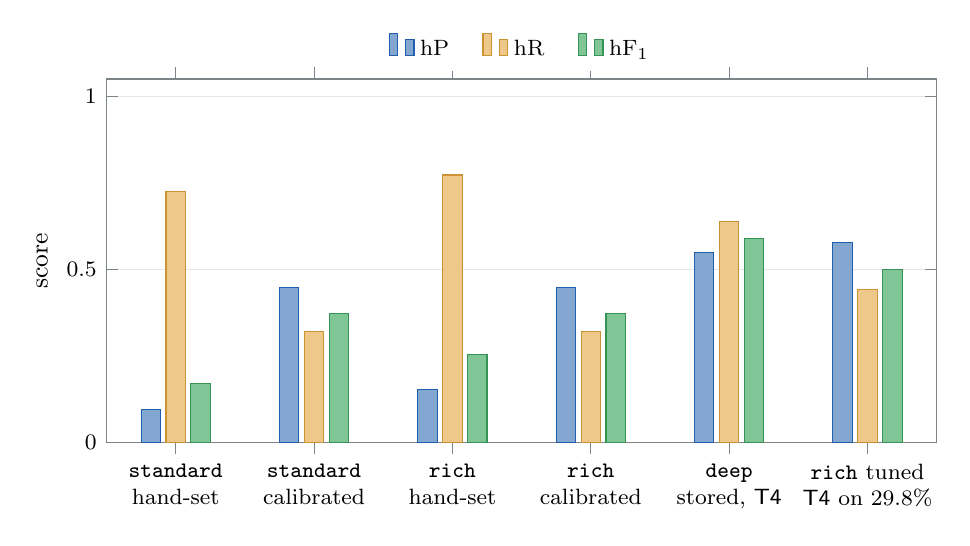
\begin{tikzpicture}
\begin{axis}[
  ybar, width=\linewidth, height=6.2cm,
  ymin=0, ymax=1.05, ylabel={score},
  symbolic x coords={sh,st,rh,rt,dp,rf},
  xtick=data,
  xticklabels={
    {\preset{standard}\\hand-set},
    {\preset{standard}\\calibrated},
    {\preset{rich}\\hand-set},
    {\preset{rich}\\calibrated},
    {\preset{deep}\\stored, \tier{4}},
    {\preset{rich} tuned\\\tier{4} on 29.8\%}},
  xticklabel style={align=center, font=\footnotesize},
  bar width=7pt, enlarge x limits=0.1,
  axis line style={ink!60}, tick style={ink!60}, ymajorgrids, grid style={ink!12},
  ticklabel style={font=\footnotesize}, label style={font=\small},
  legend style={at={(0.5,1.02)},anchor=south,legend columns=3,font=\footnotesize,draw=none,
    /tikz/every even column/.append style={column sep=10pt}},
]
\addplot[fill=accent!55, draw=accent] coordinates {(sh,0.097) (st,0.448) (rh,0.153) (rt,0.448) (dp,0.548) (rf,0.577)};
\addplot[fill=tthree!60, draw=tthree!90!black] coordinates {(sh,0.726) (st,0.320) (rh,0.773) (rt,0.321) (dp,0.639) (rf,0.442)};
\addplot[fill=ttwo!65, draw=ttwo!90!black] coordinates {(sh,0.171) (st,0.373) (rh,0.255) (rt,0.374) (dp,0.590) (rf,0.501)};
\legend{\hP, \hR, \hF}
\end{axis}
\end{tikzpicture}
\caption{Precision, recall and \hF{} of the served labels (\cref{tab:eval-quality}). Calibration trades the hand-set map's empty recall for real precision. \tier{4} on three pages in ten closes most of the gap to running it on every page.}
\label{fig:eval-quality}
\end{figure}

\tier{4} is what makes the labels good. With it on every page, \preset{deep} reaches \hF{} 0.590 on the stored profiles. The tuned \preset{rich} level of \cref{sec:cascade-tunings} gets 0.501 while sending only 29.8\% of pages to \tier{4}, and its precision, 0.577, is the highest of any level. The remaining loss is recall: a page that settles on its cheap labels never gets the labels \tier{4} would have added. The most frequent false positives at \preset{standard} before calibration were broad and generic: Genres, wrongly served on 136 of the 383 pages, Men's Fashion on 92 and Video Game Genres on 89. Per language, the tuned level scores 0.489 on English pages, 0.496 on Italian, 0.520 on French and 0.575 on the rest (\cref{tab:cascade-tunings}).

\subsection{Which model runs \tier{4}}\label{sec:eval-t4}

The cost ceiling for \tier{4} is about \$0.20 per 1,000 calls: at three pages in ten, that keeps the whole cascade within tens of dollars per million pages. A first benchmark compared 13 models on 36 pages against two frontier models used as references; it was within noise. We reran six candidates on the golden set, on the 342 judged pages whose publishers allow it, each page's real \preset{deep} prompt rebuilt with today's calibration. Each model's answers were fed back into the \preset{deep} level, and what that level served was scored against the gold. This run used the first-pass gold. \Cref{fig:eval-t4} gives the result, and \cref{tab:eval-t4} the details. The run cost \$0.52.

\begin{figure}[t]
\centering
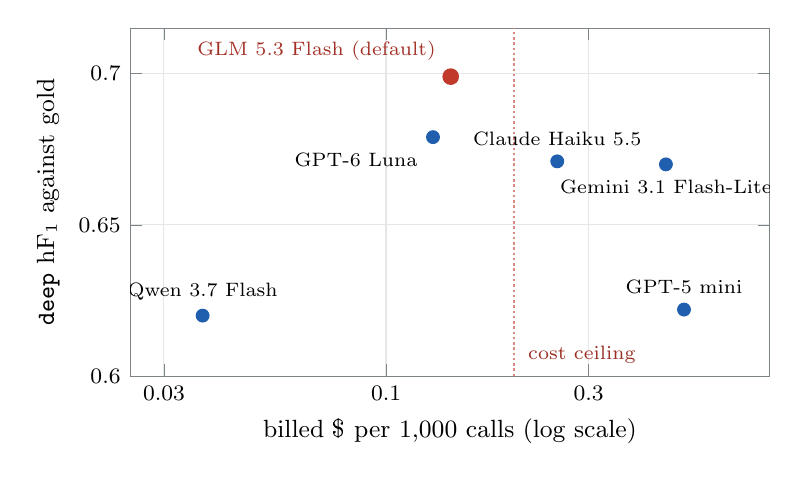
\begin{tikzpicture}
\begin{axis}[
  width=0.8\linewidth, height=6cm,
  xmode=log, xmin=0.025, xmax=0.8, ymin=0.60, ymax=0.715,
  xtick={0.03,0.1,0.3}, xticklabels={0.03,0.1,0.3},
  yticklabel style={/pgf/number format/fixed,/pgf/number format/precision=2},
  xlabel={billed \$ per 1,000 calls (log scale)}, ylabel={\preset{deep} \hF{} against gold},
  grid=major, grid style={ink!12}, axis line style={ink!60}, tick style={ink!60},
  ticklabel style={font=\footnotesize}, label style={font=\small},
]
\addplot[tfour!60, densely dotted, line width=0.9pt] coordinates {(0.2,0.60) (0.2,0.715)};
\node[font=\scriptsize, text=tfour!80!black, anchor=south west] at (axis cs:0.205,0.601) {cost ceiling};
\addplot[only marks, mark=*, mark size=2.8pt, tfour] coordinates {(0.142,0.699)};
\addplot[only marks, mark=*, mark size=2.3pt, accent] coordinates {(0.129,0.679) (0.253,0.671) (0.456,0.670) (0.503,0.622) (0.037,0.620)};
\node[font=\scriptsize, anchor=south east, text=tfour!85!black] at (axis cs:0.138,0.701) {GLM 5.3 Flash (default)};
\node[font=\scriptsize, anchor=north east] at (axis cs:0.125,0.677) {GPT-6 Luna};
\node[font=\scriptsize, anchor=south] at (axis cs:0.253,0.673) {Claude Haiku 5.5};
\node[font=\scriptsize, anchor=north] at (axis cs:0.456,0.668) {Gemini 3.1 Flash-Lite};
\node[font=\scriptsize, anchor=south] at (axis cs:0.503,0.624) {GPT-5 mini};
\node[font=\scriptsize, anchor=south] at (axis cs:0.037,0.622) {Qwen 3.7 Flash};
\end{axis}
\end{tikzpicture}
\caption{Six candidate models for \tier{4}, scored by what the \preset{deep} level serves with their answers on 342 golden pages. Without \tier{4}, the same level scores 0.145; every model lifts it to between 0.62 and 0.70. The default is both the best and under the cost ceiling.}
\label{fig:eval-t4}
\end{figure}

\begin{table}[t]
\centering\small
\caption{\tier{4} candidates on the golden set. \emph{ok}: parseable answers. \emph{kept}: labels kept per page. \emph{verified}: quotes found verbatim on the page. \tier{4} \hF: the labels the model keeps, alone. \preset{deep}: what the level serves with its answers.}
\label{tab:eval-t4}
\begin{tabular}{@{}lrrrrrrr@{}}
\toprule
Model & \$/1k calls & ok & kept & verified & \tier{4} \hF & \preset{deep} \hP & \preset{deep} \hF \\
\midrule
GLM 5.3 Flash & 0.142 & 334/342 & 2.2 & 94\% & \textbf{0.706} & \textbf{0.845} & \textbf{0.699} \\
GPT-6 Luna & 0.129 & 332/342 & 2.1 & 98\% & 0.682 & 0.832 & 0.679 \\
Claude Haiku 5.5 & 0.253 & 331/342 & 2.3 & 95\% & 0.676 & 0.810 & 0.671 \\
Gemini 3.1 Flash-Lite & 0.456 & 337/342 & 2.6 & 100\% & 0.671 & 0.747 & 0.670 \\
GPT-5 mini & 0.503 & 336/342 & 3.2 & 89\% & 0.645 & 0.657 & 0.622 \\
Qwen 3.7 Flash & 0.037 & 333/342 & 2.0 & 92\% & 0.638 & 0.801 & 0.620 \\
\bottomrule
\end{tabular}
\end{table}

Three findings matter beyond the choice. First, the gap between models is small next to the gap between having \tier{4} and not: the cheapest model is a quarter of the default's price and loses 0.08 of \hF. Second, quote verification is not free of failure even for strong models: GPT-5 mini's quotes are found on the page 89\% of the time, and halving the confidence of the others is part of why its precision is lowest. Third, prices on the catalogue are not prices on the bill. Routing only to providers that keep no prompts, the default model costs \$0.142 per 1,000 calls, against about \$0.05 at its listed price.

\subsection{What a page costs}\label{sec:eval-cost}

\Cref{tab:eval-cost} gives the cost of the tuned \preset{rich} level per million pages, from \cref{eq:cascade-cost}. \tier{4} dominates the money. Lowering its share from 49.1\% (one threshold pair everywhere) to 29.8\% (per language) saves about \$28 per million pages for 0.043 of \hF. Images cost CPU rather than money: on the three-board cluster, the two-phase rule of \cref{alg:cascade-phases} and the value budget cut the share of new pages that fetch images to 20\%, from every page before. Fetching is not in the table. At one second per site between requests and about 100\,ms a fetch, it is time and bandwidth more than money.

\begin{table}[t]
\centering\small
\caption{Cost per million pages at the tuned \preset{rich} level, with the default \tier{4} model at its billed price.}
\label{tab:eval-cost}
\begin{tabular}{@{}lrrl@{}}
\toprule
Item & Pages & \$ per million & Note \\
\midrule
\tier{0}--\tier{2} & 100\% & 6 & the cascade's estimate; CPU in practice \\
\tier{3} images & 20\% & CPU only & pages that fetch images; up to 3 each \\
\tier{4}, tuned per language & 29.8\% & 42 & \$0.142 per 1,000 calls \\
\tier{4}, one pair everywhere & 49.1\% & 70 & for comparison \\
\bottomrule
\end{tabular}
\end{table}

\subsection{Would context change what buyers do?}\label{sec:eval-reach}

The case for contextual deals is not that context finds more pages. It is that buyers bid more where the page fits what they buy. We measured this offline, on one day of an exchange's request logs, without changing anything in production. The setting is the curated deal: a buyer's deal takes requests from a list of placements, and we ask what would happen if a request whose page matches the deal's context counted too.

\paragraph{Method.} Each deal's context is inferred from its own pages: the categories that are the main topic of at least a quarter of the pages where it already passes every filter. For each deal we then look at requests its placement list alone rejected, inside the countries where it buys, and count those whose page carries the deal's context and no Sensitive Topics label. Filter reasons are logged for a sample of requests, and counts are scaled up accordingly. The pages were sampled from rejected requests and from requests each deal already received, and crawled with \tier{4} and images off. We ran this before and after the golden-set calibration.

\paragraph{Supply is not what holds deals back.} The deals with a placement list already bid on only a small fraction of the requests they are eligible for. The bottleneck is demand, so a contextual extension is worth what it changes in how often buyers bid, not merely how many requests it adds.

\paragraph{Buyers bid more on matching pages.} On requests a deal already receives, we compare the buyer's bid rate on pages that match the deal's context with its rate on pages that do not. With the hand-set calibration, buyers bid 1.8 times as often on matching pages, about four standard errors apart. After calibration the lift holds: 1.9 times with main-topic contexts, and 2.0 times with the categories the bidder's rule would actually check.

\paragraph{How much context adds.} With the hand-set calibration, a deal's context spanned so many tier-one categories under the bidder's rule that it matched nearly everything; that was an artefact of the overconfident \tier{2}. After calibration contexts are narrow, and they add a modest number of (deal, request) pairs with main-topic contexts and several times more with the rule's categories. Deals have budgets, though, and an added request is worth something only to a deal that is behind its pace. Most deals in flight were, and capping each deal's added impressions by how far behind it is and by what it has left to deliver, under-delivering deals could absorb a substantial part of what context adds. These are lower bounds: the reach pages were crawled without \tier{4}, and calibrated cheap tiers leave many pages without a main topic. A week of logs, and \tier{4} on, would firm them up.

\subsection{Coverage in practice}\label{sec:eval-coverage}

On the three-board cluster, with 3,236 stored profiles, the share of a day's impressions that fell on pages with a profile was already far larger than the share of pages those profiles cover. Coverage follows the crawl budget and the order of the frontier, since the busiest pages carry most impressions. That the crawl request on a miss reaches busy new pages within their first hour, as \cref{sec:crawl-which} says it must, is still to be measured in production.

% 10-protocol
\section{An online experiment protocol}\label{sec:protocol}

The offline results say that buyers bid more on pages that match a deal's context. They do not say that matching context makes ads work better, nor how far around a slot context reaches. Those questions need an experiment in the bidder. This section fixes its design before any data exists, so that the analysis cannot be tuned to the outcome.

\subsection{Shadow mode first}\label{sec:protocol-shadow}

The first step changes nothing. In the placements filter, where a deal rejects a request whose page is not on its list, the bidder also runs the context rule and counts, per deal, what context would have let through. Nothing is bid on those requests. The counts are the production version of the reach measurement of \cref{sec:eval-reach}, which scaled up the sample of requests whose filter reasons are logged. Only then does any arm change allocation.

\subsection{Design}\label{sec:protocol-design}

\paragraph{Unit and assignment.} The unit is the bid request, assigned by a hash of its id. No user identifier is needed, which keeps the experiment within requirement \ref{req:nouser}, and a request's arm is reproducible from its id. The test runs inside deals that opted in to ``placement list or context'' and on requests that carry the slot context of \cref{sec:boundary}, so that both treatments are possible on every unit.

\paragraph{Arms.} Three arms, crossed with the format class of the slot (\cref{fig:protocol-design}):
\begin{itemize}
\item \emph{page}: the deal's rule checks the page's profile, as the system does today;
\item \emph{slot}: the rule checks the slot's own context, the page and its nearby blocks blended by the format's kernel, with the co-visible blocks for suitability;
\item \emph{control}, 5\% of requests: no context, the placement list only. It sets the baseline for both lifts.
\end{itemize}
The format classes are scroll-through, in-article and full-screen. They differ in how much the page around the slot can count (\cref{tab:boundary-formats}), so a lift in one says little about another.

\begin{figure}[t]
\centering
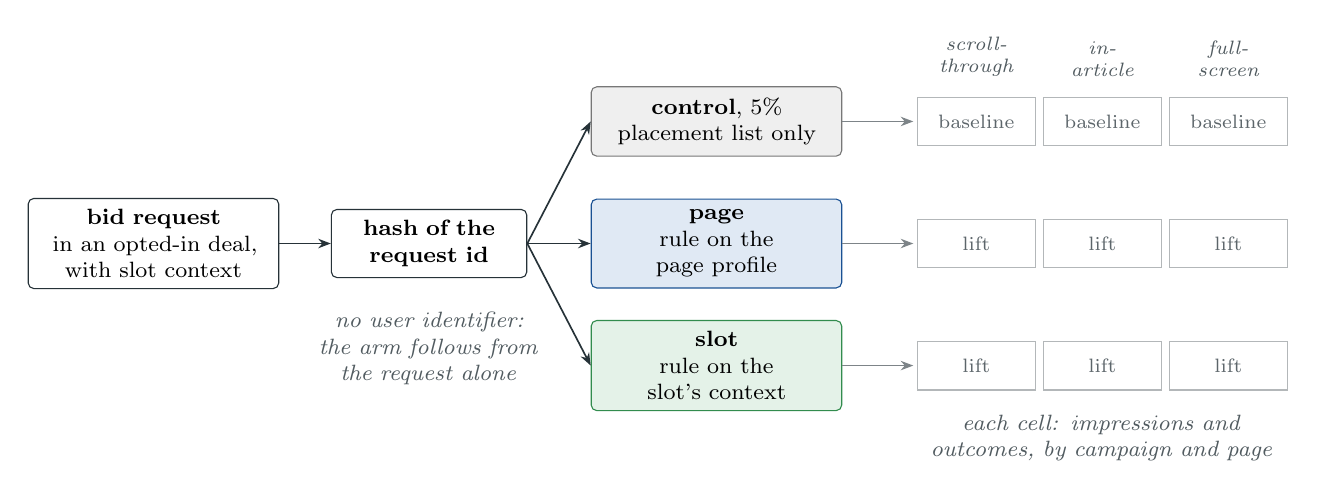
\begin{tikzpicture}[x=1cm,y=1cm,font=\footnotesize]
\tikzset{
  pbox/.style={box, fill=white, text width=#1, font=\footnotesize},
  pbox/.default=2.4cm,
  parm/.style={draw=#1!85!black, fill=#1!14, rounded corners=2pt, align=center, text width=2.9cm, inner sep=4pt, font=\footnotesize},
  pcell/.style={draw=ink!35, fill=white, minimum width=1.5cm, minimum height=0.62cm, font=\scriptsize, text=ink!75, inner sep=1pt},
  plink/.style={-{Stealth[length=1.6mm]}, semithick, draw=ink},
}
\node[pbox=2.9cm] (req) at (-0.15,0) {\textbf{bid request}\\in an opted-in deal,\\with slot context};
\node[pbox=2.2cm] (hash) at (3.35,0) {\textbf{hash of the}\\\textbf{request id}};
\draw[plink] (req) -- (hash);
\node[parm=tzero] (ctl) at (7.0,1.55) {\textbf{control}, 5\%\\placement list only};
\node[parm=accent] (pg) at (7.0,0) {\textbf{page}\\rule on the page profile};
\node[parm=ttwo] (sl) at (7.0,-1.55) {\textbf{slot}\\rule on the slot's context};
\foreach \a in {ctl,pg,sl} \draw[plink] (hash.east) -- (\a.west);
\node[font=\scriptsize\itshape, text=ink!80, align=center, anchor=south] at (10.3,2.0) {scroll-\\through};
\node[font=\scriptsize\itshape, text=ink!80, align=center, anchor=south] at (11.9,2.0) {in-\\article};
\node[font=\scriptsize\itshape, text=ink!80, align=center, anchor=south] at (13.5,2.0) {full-\\screen};
\foreach \r/\y/\t in {ctl/1.55/baseline, pg/0/lift, sl/-1.55/lift} {
  \foreach \x in {10.3,11.9,13.5} { \node[pcell] at (\x,\y) {\t}; }
  \draw[plink, draw=ink!60] (\r.east) -- (9.5,\y);
}
\node[note, anchor=north, text width=4.6cm] at (11.9,-2.05) {each cell: impressions and outcomes, by campaign and page};
\node[note, anchor=north, text width=2.8cm] at (3.35,-0.75) {no user identifier: the arm follows from the request alone};
\end{tikzpicture}
\caption{The experiment. A request is assigned to an arm by a hash of its id, then analysed within the format class of its slot. The control keeps today's placement-list behaviour; the two treatments differ only in which context the deal's rule reads.}
\label{fig:protocol-design}
\end{figure}

\paragraph{Outcomes.} The primary outcome depends on what a campaign buys, and is fixed before launch. Engagement campaigns are judged on engagement rate, creative interactions per impression. Awareness campaigns are judged on the share of impressions seen for three seconds and on dwell time, with brand-lift studies where a campaign runs one. Performance campaigns are judged on click-through and on post-click engaged sessions. Every campaign is also judged on suitability: Sensitive Topics incidents co-visible with the ad per 100,000 impressions, from an audit sample taken after the impression. That outcome also tests the co-visible rule of \cref{eq:boundary-suitability} on its own, since the page arm does not apply it.

\paragraph{What we expect.} The literature does not predict one sign. Congruent magazine ads were remembered better \citep{moorman2002effects}, so for awareness campaigns we expect the slot arm to help. Incongruent placements were sometimes processed more \citep{dahlen2008could}, so for engagement the sign is open. We write both down now so that neither can be claimed afterwards as the hypothesis.

\paragraph{Guardrails.} Context can starve a deal as easily as it can feed one. Per deal, we watch win rate, delivery pace and revenue per thousand requests against control, and an arm that pushes a deal off its pace is stopped for that deal.

\subsection{How many impressions}\label{sec:protocol-power}

Let $p_0$ be the baseline rate of the primary outcome and $\Delta$ the relative lift we want to detect, so $p_1 = p_0(1 + \Delta)$. For a two-sided test at level $0.05$ with power $0.8$, the impressions needed per arm are
\begin{equation}\label{eq:protocol-n}
  n = D \cdot \frac{(z_{0.975} + z_{0.8})^2\,\bigl[p_0(1-p_0) + p_1(1-p_1)\bigr]}{(p_1 - p_0)^2},
  \qquad z_{0.975} + z_{0.8} \approx 1.96 + 0.84,
\end{equation}
where $D$ is the design effect. Impressions cluster by page and by creative, so outcomes within a cluster are correlated and an impression carries less than one impression's worth of information. We plan on $D = 2$. \Cref{fig:protocol-power} gives $n$ for three assumed baselines. The required sample grows as $1/\Delta^2$: a 5\% lift on a 0.2\% baseline needs 3.2 million impressions per arm before clustering, a 20\% lift on a 1\% baseline needs 40,000. The test's length follows from dividing $n$ by the daily impressions of the opted-in deals that carry slot context. Formats with a low baseline need longer, or a pooled in-article cell.

\begin{figure}[t]
\centering
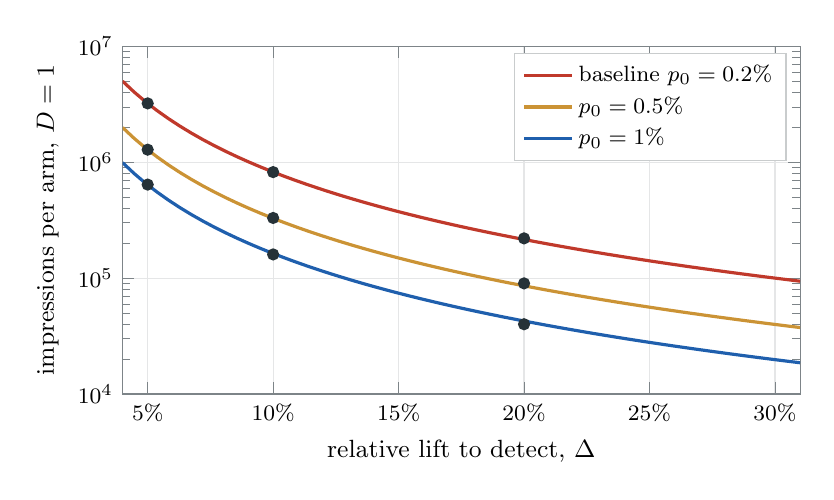
\begin{tikzpicture}
\begin{axis}[
  width=0.84\linewidth, height=6cm,
  xmin=0.04, xmax=0.31, ymode=log, ymin=1e4, ymax=1e7,
  xlabel={relative lift to detect, $\Delta$},
  ylabel={impressions per arm, $D = 1$},
  xtick={0.05,0.1,0.15,0.2,0.25,0.3},
  xticklabel={\pgfmathparse{\tick*100}\pgfmathprintnumber[fixed,precision=0]{\pgfmathresult}\%},
  grid=major, grid style={ink!12}, axis line style={ink!60}, tick style={ink!60},
  ticklabel style={font=\footnotesize}, label style={font=\small},
  legend style={at={(0.98,0.98)},anchor=north east,font=\footnotesize,draw=ink!25,fill=white},
  legend cell align=left,
  every axis plot/.append style={line width=1.15pt, samples=60, domain=0.04:0.31},
]
\addplot[tfour] {7.84*(0.002*(1-0.002) + 0.002*(1+x)*(1-0.002*(1+x)))/((0.002*x)^2)};
\addlegendentry{baseline $p_0 = 0.2\%$}
\addplot[tthree!90!black] {7.84*(0.005*(1-0.005) + 0.005*(1+x)*(1-0.005*(1+x)))/((0.005*x)^2)};
\addlegendentry{$p_0 = 0.5\%$}
\addplot[accent] {7.84*(0.01*(1-0.01) + 0.01*(1+x)*(1-0.01*(1+x)))/((0.01*x)^2)};
\addlegendentry{$p_0 = 1\%$}
\addplot[only marks, mark=*, mark size=1.6pt, ink] coordinates {(0.05,3.21e6) (0.1,0.82e6) (0.2,0.22e6) (0.05,1.28e6) (0.1,0.33e6) (0.2,0.09e6) (0.05,0.64e6) (0.1,0.16e6) (0.2,0.04e6)};
\end{axis}
\end{tikzpicture}
\caption{Impressions per arm from \cref{eq:protocol-n} before clustering, for three assumed baselines. Dots mark the planning values at 5, 10 and 20\% lift; double them for a design effect of 2. Small lifts on rare outcomes are expensive: halving the lift quadruples the sample.}
\label{fig:protocol-power}
\end{figure}

\paragraph{Analysis.} The primary analysis is a logistic regression of the outcome on the arm, within each format class, with campaign fixed effects and standard errors clustered by page. Campaign effects absorb how engaging each campaign's creatives are, so the arm's coefficient compares like with like. The two lifts, page against control and slot against control, are reported with their intervals; a difference between them is read only from their contrast, not from one being significant and the other not.

\subsection{Then fit how far context reaches}\label{sec:protocol-fit}

A first look needs no experiment. Delivery reports give impressions and engagements per site, format and advertiser category. Over 30 days, joined with the site profiles of \cref{sec:serving-backoff} for sites with at least five crawled pages, they support, per format, a binomial model
\begin{equation}\label{eq:protocol-site}
  \operatorname{logit} \mathrm{ER}_{s,c} = \alpha_c + \beta\, m_{s,c},
\end{equation}
where $\mathrm{ER}_{s,c}$ is the engagement rate of advertiser category $c$ on site $s$, $\alpha_c$ a fixed effect per category and $m_{s,c}$ the site's mean score for the \iab{} nodes the category maps to. An interval for $\beta$ above zero says that matching site context lifts engagement for that format; below zero says the reverse. A clear $\beta$ would still settle little. A site's mean profile is a blunt context, campaigns choose their sites, and category effects absorb how engaging each vertical's creatives are but not who bought where. The script that fits \cref{eq:protocol-site} exists; we report no result from it.

The experiment's logs hold, for every impression, the page's labels, the blocks around the slot with their offsets, the format and the outcome. That is enough to fit what the lab now sets by hand. Two features enter the engagement model per format: the match between the creative and the page, and the match between the creative and the local window of \cref{eq:boundary-relevance}. The kernel's reach above and below the slot, $r^{\uparrow}_f$ and $r^{\downarrow}_f$ in \cref{eq:boundary-kernel}, are profiled by likelihood. The fitted page weight and reaches are the empirical answer to the question of \cref{sec:boundary}: for this format, how far around the slot does context count?

Two things the protocol does not settle. Engagement counts interactions with the creative, which favours attention over congruence; brand recall, where congruence should matter most, needs brand-lift studies that only some campaigns run. And contextual match and obtrusive formats have each been found to raise purchase intent, but not together \citep{goldfarb2011online}. Mobile rich-media formats are obtrusive by design, so we expect the answer to differ by format, which is why every lift is read within one.

% 11-discussion
\section{Discussion, limitations and ethics}\label{sec:discussion}

We set six requirements in \cref{sec:overview}. \Cref{tab:discussion-reqs} says, for each, what the system does about it and what is still unshown. The pattern is plain. What can be checked in a test or a benchmark holds. What needs a reader, an impression or a week of traffic has been designed but not yet measured.

\begin{table}[t]
\centering\small
\caption{The requirements of \cref{sec:overview}, what meets them and what is open.}
\label{tab:discussion-reqs}
\begin{tabularx}{\linewidth}{@{}l>{\raggedright\arraybackslash}X>{\raggedright\arraybackslash}X@{}}
\toprule
Requirement & What meets it & Open \\
\midrule
\ref{req:latency} latency & one key-value read per backoff level; decode 83\,ns and a rule check 9\,ns, both without allocation; slot context 1.8\,\textmu s (\cref{tab:serving-sdk}) & the read inside a production bidder, under its load \\
\ref{req:cost} cost & the value budget and per-language thresholds: \tier{4} on 29.8\% of pages, about \$42 per million (\cref{tab:eval-cost}) & thresholds refitted on a fresh crawl; a batch API \\
\ref{req:fresh} freshness & a crawl request on every miss, value-ordered frontier, SimHash refresh (\cref{sec:crawl}) & time to first profile for busy new pages, in production \\
\ref{req:explain} explanations & every decision names its deciding label; full traces on demand & an audit store keyed by URL, content hash and version \\
\ref{req:sensitive} suitability & worst case over everything co-visible (\cref{eq:boundary-suitability}); never blended & incidents per impression, from the experiment \\
\ref{req:nouser} no user data & by construction: inputs are the page and the slot & none \\
\bottomrule
\end{tabularx}
\end{table}

\subsection{What the evaluation does not show}\label{sec:discussion-limits}

\paragraph{The gold labels come from a model.} This is the largest gap, and we repeat it from \cref{sec:eval-golden}. An LLM judged the golden pages, and \tier{4} is an LLM. Part of what \cref{tab:eval-quality} measures is agreement between two models, which flatters \tier{4} and whatever was calibrated against it. The remedy is cheap and not yet done: judge 50 pages by hand in the lab and measure agreement with the gold before trusting any finer calibration to it. Until then, differences of a few hundredths of \hF{} between settings are within what a different judge could move.

\paragraph{The sample is small and follows the exchange.} 383 pages from 25 publishers carry the whole quality evaluation. They follow the supply of one exchange: four main languages, many homepages, no Spanish at all and only 27 German pages. Spanish and German share a fallback calibration and threshold pair. A different exchange, or the same one a year later, would weight the languages and page types differently, and the tunings would move with them.

\paragraph{The tunings may be overfitted.} \Cref{sec:cascade-tunings} fits each language's thresholds by trying 140 choices on 31 to 164 pages, and evaluates on the same pages. With so few pages per language, the trade we measured for per-language thresholds, \$28 per million pages saved for 0.043 of \hF{}, may not hold on new pages. The fit also used \tier{4} outcomes from an older crawl, on older shortlists. A recrawl with the audit trace on, then a refit with pages held out, would answer both concerns.

\paragraph{The shortlist caps \tier{4}.} \tier{4} chooses among the 12 labels that \tier{0}--\tier{3} rank highest. If $G$ is a page's gold set and $S_{12}$ the shortlist, every label \tier{4} returns lies in $S_{12}$, so its flat recall on that page is at most
\begin{equation}\label{eq:discussion-cap}
  R_{\tier{4}} \le \frac{|G \cap S_{12}|}{|G|}.
\end{equation}
Pooled over pages, the bound is the share of the 1,173 gold labels found in the shortlists, the recall@12 of \cref{fig:cascade-recall}: 62.7\%, or 64.8\% on the shortlists the model actually saw. Hierarchical recall is a little kinder, since an ancestor in the shortlist earns partial credit. The stored \preset{deep} profiles reach \hR{} 0.639, close to the bound, which suggests that most of what \tier{4} misses was never offered to it. A longer shortlist is not the fix. Recall at 96 labels is 93.1\%, with eight times as many labels in every prompt. The ranking of the lower tiers is what has to improve. Distilling \tier{4}'s labels back into \tier{1}'s term weights and into a learned \tier{2} head is the planned route.

\paragraph{Bids are not outcomes.} \Cref{sec:eval-reach} shows that buyers bid about twice as often on pages that match a deal's context. That is evidence that the profiles describe something buyers care about. It is not evidence that ads on those pages work better, and it is observational: a deal's matching pages may also be its better sites. The sample was one day, with filter reasons logged for a sample of requests and \tier{4} off. The causal question goes to the experiment of \cref{sec:protocol}, which has not run.

\paragraph{The slot priors are hand-set.} Every number in \cref{eq:boundary-odds} and every page weight and reach of \cref{tab:boundary-formats} is a plausible guess marked as such in the code (\cref{sec:boundary-odds}). The slot machinery is tested for agreement between its two implementations, not for being right about readers. The experiment's logs are what should replace the guesses.

\paragraph{Some publishers cannot be crawled.} Of the 469 pages drawn, 86 answered with HTTP 403 or were disallowed by robots.txt, and four of the 25 publishers gave us nothing. Some of these refuse any crawler they do not know. A crawler with a public information page, published address ranges and signed requests would be known; until it is, part of the supply has no profile and falls back to the section, the site or nothing.

\paragraph{The crawler reads markup, not pixels.} We do not render pages. Content that only scripts insert, ad containers injected late and the real heights of blocks are estimated or missed. The page module measures what the browser lays out, but only where a publisher runs it. Homepages change by the hour, carry many impressions and are the hardest pages here: what a slot on a homepage sits next to is a teaser, and a profile of the whole page says little about it.

\paragraph{No external comparison.} We have not compared profiles with a commercial verification service on the same URLs. Such a comparison would not give ground truth either, but it would say whether our Sensitive Topics verdicts are in line with what buyers already accept.

\subsection{What carries over}\label{sec:discussion-general}

Two parts of the design do not depend on advertising. The cascade with a value budget applies wherever a large, skewed stream of documents must be labelled against a fixed taxonomy and the expensive judge can be afforded on only a fraction: spend follows the value of the item, cheap tiers settle what they can, and every decision keeps its deciding evidence. The slot model applies wherever a decision depends on part of a document rather than all of it. It separates the question of relevance, a weighted blend, from the question of suitability, a worst case, and the separation is what keeps one sensitive headline from being averaged away. The specific numbers, from the 704 nodes to the kernel's reach, belong to this exchange and this taxonomy. The structure does not.

\subsection{Ethics}\label{sec:discussion-ethics}

\paragraph{Users.} No cookie, user identifier, device identifier or browsing history enters a profile or a decision, and the experiment assigns by request, not by user. We dropped one idea for this reason: using the previous page as context for an interstitial would bring in a reader's history and the consent obligations that come with it (\cref{sec:boundary-status}). Contextual advertising is not free of privacy questions, since a page can reveal a reader's interests, but the system adds nothing about the reader to what the bid request already carries.

\paragraph{Publishers.} The crawler honours robots.txt under RFC~9309, treats an unreachable file as a refusal, waits at least a second between requests to a host and revalidates with conditional requests where it can. Before any page text goes to a generative model, the AI-use gate of \cref{sec:crawl-gate} reads the publisher's stated preferences and licence, and a refusal anywhere wins. On the golden sample 41 of 383 stored pages were denied, and they were classified without \tier{4}. A licence we cannot negotiate yet counts as a refusal. We think the default should lean this way while the conventions settle: classifying a page to sell ads on it benefits the publisher, but sending its text to a third-party model is a use the publisher should be able to refuse.

\paragraph{The pages that are labelled.} Suitability labels decide where money goes. A page labelled with a Sensitive Topic loses the deals that block it, and news about crime, war or disease is exactly the content such labels catch. Over-blocking takes revenue from journalism that is often the most expensive to produce. Two choices in \sys{} limit this. Deals block Sensitive Topics, not keywords, so a page is blocked for what it is about rather than for a word in it. And every block names its deciding label and evidence, so a publisher or a trader can see why a page was refused and dispute it. Whether the labels are calibrated well enough on hard news is a question the human check above should answer specifically.

\paragraph{The models.} We used an LLM both to classify and to judge, and we report the cost of both. Page text was sent to hosted models through an API; no user data was. The golden set's URLs and judgements come from an exchange's traffic and are not published, so these results cannot be audited page by page from outside. The code (\repo) holds a made-up pair of files in the same format, so anyone can run the same evaluation on a sample of their own. The pages' text is not ours to publish either.

% 12-conclusion
\section{Conclusion}\label{sec:conclusion}

A bidder that buys on context has to know, inside each bid, what the reader is looking at. \sys{} answers with a profile per page, computed offline, and a slot context computed at bid time where the page reports it. Three ideas carry the design. Spend on a page follows what the page is worth, so the language model is called on fewer than a third of pages and the cascade costs tens of dollars per million. Every label carries the evidence that produced it, so a refusal can be read and checked. And relevance and suitability are different questions: the first blends the page with what is near the slot, the second takes the worst of everything on screen with the ad.

The numbers we can stand behind are the ones a test or a log can check: latency in nanoseconds to microseconds, the cost per million pages, the bound that the shortlist puts on the last tier, and buyers bidding about twice as often on pages that match. The ones we cannot yet stand behind need people or impressions: golden labels judged by hand, and the experiment of \cref{sec:protocol}, which would say whether slot context changes what ads do and how far around a slot context reaches. Both are designed. Neither has run. We expect the structure to survive what they find, because the parts they would change, the thresholds, the kernel's reach and the page weight per format, are parameters rather than structure.


\bibliographystyle{plainnat}
\bibliography{refs-related,refs-cascade,refs-boundary}

\appendix
% a1-wire
\section{Profile wire format and interfaces}\label{app:wire}

\Cref{lst:wire-proto} is the serving profile the bidder reads
(\code{src/protos/contextual/v1/profile.proto}), with its comments shortened.
Two encoding choices matter for size. Scores are 32-bit floats, which is more
precision than a calibrated score in $[0, 1]$ needs and costs 5 bytes with its
tag. SimHashes are \code{fixed64}: a hash is close to uniform over 64 bits, and a
varint of such a value takes 9 or 10 bytes, where a fixed field always takes
8. The Go reader skips any field it does not know, so fields can be added
without a coordinated release.

\begin{lstlisting}[caption={The serving profile, \code{contextual.v1.PageProfile}.},label={lst:wire-proto},captionpos=b,columns=fixed,basewidth=0.5em,keepspaces=true]
syntax = "proto3";
package contextual.v1;

// A page's profile under contextual:<sha256(normalised URL)>. The same message
// under contextual:section:<sha256(prefix)> is a top section's or a site's
// profile: the mean of its crawled pages' scores, from 5 pages on, no keywords.
message PageProfile {
  // IAB Content Taxonomy 3.1 (cattax 9) ids, highest score first, calibrated
  // to [0, 1], at most 20. Every label's ancestors are in the list too, with
  // at least its score: a category matches when its own id is here.
  repeated Label labels = 1;
  repeated string keywords = 2;  // at most 20, most salient first
  int64 fetched_at = 3;          // Unix seconds
  string preset = 4;             // the cascade depth the labels come from: "rich"
  string version = 5;            // pipeline version, for logs and audits
  // Labelled blocks in document order, at most 64: what a slot's own context
  // is made of (ortb2Imp.ext.data.ctx). No text, only its SimHash.
  repeated Block blocks = 6;
  // Ad containers and where each sits: a slot's surroundings when the bid
  // request carries no ext.data.ctx.
  repeated AdSlot ad_slots = 7;
}

message AdSlot {
  string id = 1;   // the container's element id: the part of a GPID after its last #
  float top = 2;   // the bottom of the block before it, viewports from the top
}

message Block {
  fixed64 simhash = 1;        // of its words: a rendered block is this one
                              // when at most 3 bits differ
  bool main = 2;              // main content; false for navigation, widgets, comments
  repeated Label labels = 3;  // its best labels (at most 8), ancestors included
  float top = 4;              // its middle, viewports from the top, as estimated
}

message Label {
  string id = 1;     // IAB Content Taxonomy 3.1 unique id
  float score = 2;   // in [0, 1]
}
\end{lstlisting}

The crawlers and online servers share one store, Valkey in the lab
(\cref{tab:wire-keys}). Every multi-key step of the crawl frontier is one Lua
script, so it is atomic across replicas. Only the two \code{contextual:} key
families are meant for the bidder. Everything under \code{ctx:} is the lab's
own state.

\begin{table}[ht]
\centering
\caption{Key families in the shared store (\code{src/serve/lab.ml}). Expiries
  are given where a key has one.}
\label{tab:wire-keys}
\footnotesize
\begin{tabularx}{\linewidth}{@{}l l >{\raggedright\arraybackslash}X@{}}
\toprule
Key & Type & Holds\\
\midrule
\multicolumn{3}{@{}l}{\emph{Read by the bidder}}\\
\code{contextual:<sha256>} & string & the page's \code{PageProfile}; 30 days\\
\code{contextual:section:<sha256(prefix)>} & string & a top section's or site's mean \code{PageProfile}, from 5 pages; 30 days\\
\midrule
\multicolumn{3}{@{}l}{\emph{Crawl frontier and politeness}}\\
\code{ctx:seen} & set & normalised URL keys ever queued\\
\code{ctx:frontier:<origin>} & sorted set & URLs waiting for that origin, scored by minus their bid requests per day\\
\code{ctx:hosts} & sorted set & origins with work, scored by their earliest next fetch\\
\code{ctx:hints} & hash & URL to its sitemap hints, while queued\\
\code{ctx:inflight} & hash & URL to its origin, claim time and frontier score\\
\code{ctx:stats}, \code{ctx:recent} & hash, list & counters and LLM spend; the last 100 outcomes\\
\code{ctx:replicas}, \code{ctx:crawled\_by} & sorted set, hash & crawler heartbeats; pages crawled per crawler\\
\midrule
\multicolumn{3}{@{}l}{\emph{Profiles, sections and refresh}}\\
\code{ctx:profile:<key>} & string & the lab's full profile, JSON, zstd-compressed\\
\code{ctx:profiles} & sorted set & profile keys by fetch time, for incremental reloads\\
\code{ctx:summary} & hash & key to a page summary with its served labels\\
\code{ctx:section:<prefix>} & hash & \code{\#pages} and the sum of the pages' served scores per label\\
\code{ctx:fresh}, \code{ctx:refresh} & hash, sorted set & refresh state per page; when to fetch it again\\
\code{ctx:requests} & hash & key to the latest known bid requests per day\\
\code{ctx:slotmap:<version>:<template>} & hash & ad container and page to main blocks before it; 30 days\\
\midrule
\multicolumn{3}{@{}l}{\emph{Archives, caches and the golden set}}\\
\code{ctx:warc}, \code{ctx:warcfile:<f>} & hash, set & where each page's raw WARC record is\\
\code{ctx:robots:<origin>} & string & robots.txt body; 24 hours\\
\code{ctx:license:<url>} & string & an RSL document, for its \code{max-age}\\
\code{ctx:image:<patches>:<sha256(src)>} & string & a SigLIP 2 image embedding, float32; 30 days\\
\code{ctx:adjudication} & hash & URL to its golden-set judgement\\
\bottomrule
\end{tabularx}
\end{table}

Both daemons speak JSON over HTTP (\cref{tab:wire-http}). Errors come back as
\code{\{"error": "..."\}}, with status 400 for bad input and 404 for unknown
pages or routes. The online server proxies every \code{/crawler/*} path to the
crawl daemon, so the front end talks to one origin. \code{level} is one of the
four presets, \preset{standard} by default, and \code{format} is one of the
five classes of \cref{tab:boundary-formats}, \code{scroll-through} by default.

\begin{table}[ht]
\centering
\caption{HTTP endpoints of the crawl daemon and the online server
  (\code{docs/guide/api.md}).}
\label{tab:wire-http}
\footnotesize
\begin{tabularx}{\linewidth}{@{}l >{\raggedright\arraybackslash}X@{}}
\toprule
Endpoint & What it does\\
\midrule
\multicolumn{2}{@{}l}{\emph{Crawl daemon, port 8081}}\\
\code{POST /crawl} & queue pages (\code{url}, \code{urls}, \code{force}, \code{requests}) or discover a site from its sitemaps (\code{site}, \code{max\_pages})\\
\code{POST /traffic} & queue the pages the bidder sees most, one \code{url<TAB>requests per day} line each, busiest first\\
\code{POST /coverage} & the same lines; how much of that traffic lands on pages with a profile\\
\code{POST /sections} & add pages stored before section profiles existed to the running sums\\
\code{GET /status} & queue, in flight, stored, live replicas, the last 100 outcomes, LLM calls and spend\\
\code{GET /pages} & one summary per stored profile\\
\code{GET /inspect?url=} & the stored profile and the cascade trace for each preset\\
\code{GET /record?url=} & the page's latest raw record, if this replica archived it\\
\code{POST /replay} & classify this replica's archived pages again, without fetching\\
\midrule
\multicolumn{2}{@{}l}{\emph{Online server, port 8080}}\\
\code{GET /api/pages?level=} & every crawled page with its top labels at that level\\
\code{GET /api/page?url=} & one page: levels, labels with evidence, segments with positions, gold labels\\
\code{POST /api/placement} & slot odds for a creative described in words on one page, with backoff to section or site and optional measured geometry\\
\code{POST /api/outreach} & the pages whose best slot reaches a fit threshold, with a histogram and a table per site\\
\code{GET /replay?url=} & the archived page, made safe to frame: scripts, objects and frames forbidden\\
\code{GET}, \code{POST}, \code{DELETE /api/adjudication} & read, save or forget a page's golden-set judgement\\
\code{GET /api/adjudication.tsv} & every judgement\\
\code{GET /api/golden} & each level's hierarchical agreement with the judgements\\
\code{GET /api/taxonomy?q=} & up to 20 categories whose path contains \code{q}\\
\bottomrule
\end{tabularx}
\end{table}

% a2-slot
\section{Slot context on the wire}\label{app:slot}

The page module writes one JSON object per ad unit into
\code{ortb2Imp.ext.data.ctx}. This example is the one in the module's README;
its two hashes are those of the first two fixture texts of
\cref{tab:slot-fixtures}:
\begin{lstlisting}
"ortb2Imp": {"ext": {"data": {"ctx": {"v": 1, "vh": 844,
  "b": [["28b95a9f8d39808e", -0.42], ["0f0127458431a25e", 0.31]]}}}}
\end{lstlisting}
\code{v} is the format's version, 1. \code{vh} is the viewport height in CSS
pixels, rounded. \code{b} lists up to $k$ blocks, nearest first, each as its
SimHash in 16 hexadecimal digits and its offset in viewports, rounded to two
decimals: from the slot's top to the block's middle, negative above. With the
defaults $k = 12$ and a reach of 3 viewports, each entry takes at most 26
characters, and the whole object stays under 350 bytes. The module is configured
in Prebid.js's real-time data block, for instance with an auction delay of
20\,ms, and any error leaves that ad unit without \code{ctx} rather than
holding the auction back.

\begin{algorithm}[ht]
\caption{The page module, for one ad unit (\code{slotContext} in \code{sdks/prebid}).}
\label{alg:slot-module}
\begin{algorithmic}[1]
\Require ad unit $a$; $k = 12$; reach $R = 3$
\State $id \gets$ the part of $a$'s GPID after its last \code{\#}, else $a$'s code
\State $e \gets$ the element with id $id$; \Return nothing if absent or the viewport height $H$ is 0
\State $y \gets$ top of $e$ in page coordinates
\ForAll{elements $x$ matching \code{h1, h2, h3, p, li, blockquote, figcaption}}
  \State \textbf{skip} $x$ if it lies inside $e$, is not rendered, or its own text has fewer than 20 characters
  \State $d_x \gets (m_x - y) / H$, with $m_x$ the middle of $x$; keep $x$ if $|d_x| \le R$
\EndFor
\State sort the kept blocks by $|d_x|$ and take the first $k$
\State \Return $\{$\code{v}: 1, \code{vh}: $H$, \code{b}: $[(\operatorname{simhash}(\text{own text of } x),\ \operatorname{round}_2(d_x)), \dots]\}$
\end{algorithmic}
\end{algorithm}

A block's own text leaves out nested blocks, scripts and styles, so text inside
a nested block counts only for that block, as in the crawler's extractor.
Runs of whitespace are squashed to single spaces before the 20-character test.

\subsection{The hash}\label{app:slot-hash}

Both sides hash the same words. The tokeniser is BERT's basic normaliser,
written in C for the crawler and in JavaScript for the module. It drops control
and format characters, turns any whitespace into a space and makes each CJK
ideograph a word of its own. It lowercases, decomposes each character
(Unicode NFD) and drops the combining marks, which strips accents. Unicode
punctuation, and every printable ASCII character that is not a letter or a
digit, separates words and is dropped. Other symbols stay, so \code{\textsterling 2.5bn}
gives the words \code{\textsterling 2} and \code{5bn}.

Each word $w$ is hashed with 64-bit FNV-1a over its UTF-8 bytes
$c_1 \dots c_m$:
\begin{equation}\label{eq:slot-fnv}
h_0 = \mathtt{0xcbf29ce484222325},\qquad
h_j = (h_{j-1} \oplus c_j)\cdot \mathtt{0x100000001b3} \bmod 2^{64},\qquad
h(w) = h_m.
\end{equation}
Every occurrence of a word then votes on every bit
\citep{charikar2002similarity}. With $W$ the block's words in order, repeats
included, and $h_i(w)$ bit $i$ of $h(w)$,
\begin{equation}\label{eq:slot-simhash}
V_i = \sum_{w \in W} \bigl(2\,h_i(w) - 1\bigr),\qquad
\operatorname{simhash}_i = [\,V_i > 0\,],\qquad i = 0, \dots, 63,
\end{equation}
so a tie sets the bit to 0. Only the words count: case, accents, punctuation
and word order do not. \code{The derby ends 2-1.}\ and \code{the DERBY ends 2 1}
both hash to \code{a767ac4cc601b1dd}. The crawler uses the same hash, over a
page's main text, to decide whether a page changed between fetches
(\cref{sec:crawl}). The module's output is pinned to the crawler's by 25 texts
that the OCaml side writes, in five languages, with typographic punctuation,
accents, digits, CJK, symbols and emoji (\cref{tab:slot-fixtures}).

\begin{table}[ht]
\centering
\caption{Three of the 25 fixture texts, their words as both tokenisers see
  them, and their SimHash (\code{sdks/prebid/test/simhash.tsv}).}
\label{tab:slot-fixtures}
\footnotesize
\begin{tabularx}{\linewidth}{@{}>{\raggedright\arraybackslash}X >{\raggedright\arraybackslash}X l@{}}
\toprule
Text & Words & SimHash\\
\midrule
Marcus Thuram prima di Feyenoord-Inter: \guillemotleft Abbiamo sbagliato, ora dobbiamo vincere\guillemotright &
  \code{marcus thuram prima di feyenoord inter abbiamo sbagliato ora dobbiamo vincere} & \code{28b95a9f8d39808e}\\
L'ÉCONOMIE française résiste : la Banque de France relève sa prévision de croissance à 1,2 \% &
  \code{l economie francaise resiste la banque de france releve sa prevision de croissance a 1 2} & \code{0f0127458431a25e}\\
Breaking: Prime Minister announces \textsterling 2.5bn package for the NHS after winter crisis &
  \code{breaking prime minister announces \textsterling 2 5bn package for the nhs after winter crisis} & \code{67d1711824c96098}\\
\bottomrule
\end{tabularx}
\end{table}

\subsection{Matching at the bidder}\label{app:slot-match}

Let the request name blocks $(g_j, d_j)$ and let the served profile hold
blocks $b_1, \dots, b_n$ in document order, with hashes $h_{b_i}$. Each request
block is matched on its own to the nearest profile block in Hamming distance,
\begin{equation}\label{eq:slot-match}
i^\ast(j) = \min\Bigl(\operatorname*{arg\,min}_{i}\ \operatorname{popcount}(g_j \oplus h_{b_i})\Bigr),
\qquad \text{accepted when } \operatorname{popcount}(g_j \oplus h_{b_{i^\ast}}) \le 3,
\end{equation}
where the outer minimum breaks ties in favour of the earlier block. An
accepted match lends the request block its \code{main} flag and labels; its
offset stays $d_j$, as the browser measured it. A request block with no match
within 3 bits counts as main content with no labels, so it dilutes the
neighbourhood in \cref{eq:boundary-relevance} and can never make the slot
safer (\cref{prop:boundary-monotone}). Nothing stops two request blocks from
matching the same profile block. That is harmless: identical texts have
identical hashes, and a block's labels depend only on its text and the page's
language, so any copy carries the same labels.

The threshold of 3 bits is the one the crawler uses for change detection,
after \citet{manku2007detecting}. For two independent, uniform 64-bit hashes
the chance of a match by accident is
\begin{equation}\label{eq:slot-false}
2^{-64} \sum_{k=0}^{3} \binom{64}{k} = \frac{43{,}745}{2^{64}} < 3 \times 10^{-15},
\end{equation}
so a request with 12 blocks against a profile with 64 is very unlikely to
pair unrelated texts. The real risk runs the other way. A block edited after
the crawl may move more than 3 bits, and a short paragraph can do so with one
changed word. Such a block then counts as unknown. We have not measured how
often that happens on live pages.

Without \code{ctx}, \code{Profile.SlotOfGPID} builds the same list from the
profile: it takes the container named by the GPID, computes each labelled
block's offset from the container's estimated top, keeps those within 3
viewports and returns the 12 nearest, sorted by distance with ties kept in
document order. The Go function and the OCaml \code{Profile.gpid\_slot} agree
on 1,000 fixture cases.

\end{document}
